\documentclass[hidelinks,brazil,tese,epusp]{usp}
\usepackage[T1]{fontenc}  %Orienta a saída do texto a reproduzir caracteres especiais
\usepackage[utf8]{inputenc} %Permite que o usuário redija o documento utilizando caracteres especiais UTF-8

\usepackage{graphicx}  %Pacote de gerenciamento de figuras. Padrão para qualquer documento em LaTeX
\usepackage{helvet}  %Define Helvetica como fonte Sans Serif padrão
\usepackage{fancyvrb}  %Serve, por exemplo para aplicar estilos de texto individuais em trechos do texto
\usepackage{babel}  %Pacote de idioma
\usepackage{textcomp}  %Graças a esse pacote eu não preciso me preocupar com o símbolo °
%\usepackage{textgreek} %Define comandos para chamar letras gregas. Passei a usar o modo matemático pra isso.
%\usepackage{fixltx2e}  %Define \textsubscript{}, por exemplo.
\usepackage[font=normalsize]{subfig}  %Habilita utilização de subfiguras nos campos de figuras.
\usepackage{indentfirst}  %Faz a primeira linha após o chapter head ser indentada (vide definição de \thickline abaixo)
\usepackage{array}  %Graças a ele eu consigo editar elementos de tabela.
\usepackage{amsmath}  %Pacote com complementos do modo matemático.
\usepackage[symbolgreek]{mathastext}  %Equações ficam na mesma fonte do texto graças a isso. http://jf.burnol.free.fr/v13/mathastext.pdf
%\usepackage{paralist}  %Possibilita a criação de listas (ambiente enumerate) "inline".
\usepackage[hang,flushmargin]{footmisc}  %Deixa a indentação do rodapé do jeito que eu quero (vide exemplos no texto).
\usepackage{enumerate}  %Formata rótulos de listas enumeradas

\usepackage{siunitx}  %Formatação grandezas sistema internacional
\sisetup{output-decimal-marker={,}}

\usepackage{multirow}  %Multi colunas e multi linhas em tabelas

\makeatletter
%%% Macro incrível que peguei no http://tex.stackexchange.com/questions/101002/interrupting-and-resuming-subequations
%%% para parar e retomar subequações no LaTeX. Fantástico!
\def\user@resume{resume}
\def\user@intermezzo{intermezzo}
%
\newcounter{previousequation}
\newcounter{lastsubequation}
\newcounter{savedparentequation}
\setcounter{savedparentequation}{1}
% 
\renewenvironment{subequations}[1][]{%
  \def\user@decides{#1}%
  \setcounter{previousequation}{\value{equation}}%
  \ifx\user@decides\user@resume 
    \setcounter{equation}{\value{savedparentequation}}%
  \else  
  \ifx\user@decides\user@intermezzo
    \refstepcounter{equation}%
  \else
    \setcounter{lastsubequation}{0}%
    \refstepcounter{equation}%
  \fi\fi
  \protected@edef\theHparentequation{%
  \@ifundefined {theHequation}\theequation \theHequation}%
  \protected@edef\theparentequation{\theequation}%
  \setcounter{parentequation}{\value{equation}}%
  \ifx\user@decides\user@resume 
    \setcounter{equation}{\value{lastsubequation}}%
  \else
    \setcounter{equation}{0}%
  \fi
  \def\theequation  {\theparentequation  \alph{equation}}%
  \def\theHequation {\theHparentequation \alph{equation}}%
  \ignorespaces
}{%
%  \arabic{equation};\arabic{savedparentequation};\arabic{lastsubequation}
  \ifx\user@decides\user@resume
    \setcounter{lastsubequation}{\value{equation}}%
    \setcounter{equation}{\value{previousequation}}%
  \else
  \ifx\user@decides\user@intermezzo
    \setcounter{equation}{\value{parentequation}}%
  \else
    \setcounter{lastsubequation}{\value{equation}}%
    \setcounter{savedparentequation}{\value{parentequation}}%
    \setcounter{equation}{\value{parentequation}}%
  \fi\fi
%  \arabic{equation};\arabic{savedparentequation};\arabic{lastsubequation}
  \ignorespacesafterend
}
%%% Termina aqui a macro

%%%Define linhas horizontais (\thickline) e verticais (') para tabelas
\newcommand{\thickhline}{
  \noalign {\ifnum 0=`}\fi \hrule height 1.5pt
  \futurelet \reserved@a \@xhline
}
\newcolumntype{'}{@{\hskip\tabcolsep\vrule width 1.5pt\hskip\tabcolsep}}
\makeatother

\begin{document}
\bibliographystyle{usp}

\titulo{Têmpera e Partição de ferros fundidos nodulares: microestrutura e cinética}
\autor{Arthur Seiji Nishikawa}
\orientador{Prof. Dr. Hélio Goldenstein}
\coorientador{Prof. Dr. André Paulo Tschiptschin}
\programa{3133}
\departamento{ep-pmt}

\resumo{
  \setlength\parindent{0pt}
  Este trabalho está inserido em um projeto que procura estudar a viabilidade técnica da aplicação de um relativamente novo conceito de tratamento térmico, chamado de Têmpera e Partição (T\&P), como alternativa para o processamento de ferros fundidos nodulares com alta resistência mecânica. O processo T\&P tem por objetivo a obtenção de microestruturas multifásicas constituídas de martensita e austenita retida, estabilizada em carbono. A martensita confere elevada resistência mecânica, enquanto a austenita confere ductilidade. No processo T\&P, após a austenitização total ou parcial da liga, o material é temperado até uma temperatura de têmpera $T_T$ entre as temperaturas Ms e Mf para produzir uma mistura controlada de martensita e austenita. Em seguida, na etapa de partição, o material é mantido isotermicamente em uma temperatura igual ou mais elevada (denominada temperatura de partição $T_P$) para permitir a partição de carbono da martensita para a austenita. O carbono em solução sólida diminui a temperatura Ms da austenita, estabilizando-a à temperatura ambiente. O presente trabalho procurou estudar aspectos de transformações de fases --- com ênfase na evolução microestrutural e cinética das reações --- do tratamento térmico de Têmpera e Partição (T\&P) aplicado a uma liga de ferro fundido nodular (Fe--3,47\%C--2,47\%Si--0,2\%Mn). Tratamentos térmicos consistiram de austenitização a \SI{880}{\degreeCelsius} por 30~min, seguido de têmpera a 140, 170 e \SI{200}{\degreeCelsius} e partição a 300, 375 e \SI{450}{\degreeCelsius} por até 2~h. A caracterização microestrutural foi feita por microscopia óptica (MO), eletrônica de varredura (MEV), difração de elétrons retroespalhados (EBSD) e análise de microssonda eletrônica (EPMA). A análise cinética foi feita por meio de ensaios de dilatometria de alta resolução e difração de raios X in situ usando radiação síncrotron. Resultados mostram que a ocorrência de reações competitivas --- reação bainítica e precipitação de carbonetos na martensita --- é inevitável durante a aplicação do tratamento T\&P à presente liga de ferro fundido nodular. A cinética da reação bainítica é acelerada pela presença da martensita formada na etapa de têmpera. A reação bainítica acontece, a baixas temperaturas, desacompanhada da precipitação de carbonetos e contribui para o enriquecimento em carbono, e consequente estabilização, da austenita. Devido à precipitação de carbonetos na martensita, a formação de ferrita bainítica é o principal mecanismo de enriquecimento em carbono da austenita. A microssegregação proveniente da etapa de solidificação permanece no material tratado termicamente e afeta a distribuição da martensita formada na etapa de têmpera e a cinética da reação bainítica. Em regiões correspondentes a contornos de célula eutética são observadas menores quantidades de martensita e a reação bainítica é mais lenta. A microestrutura final produzida pelo tratamento T\&P aplicado ao ferro fundido consiste de martensita revenida com carbonetos, ferrita banítica e austenita enriquecida estabilizada pelo carbono. Adicionalmente, foi desenvolvido um modelo computacional que calcula a redistribuição local de carbono durante a etapa de partição do tratamento T\&P, assumindo os efeitos da precipitação de carbonetos e a ocorrência do crescimento de placas de ferrita bainítica a partir da austenita. O modelo mostrou que a cinética de partição de carbono da martensita para a austenita é mais lenta quando os carbonetos precipitados são mais estáveis e que, quando a energia livre dos carbonetos é suficientemente baixa, o fluxo de carbono acontece da austenita para a martensita. A aplicação do modelo não se limita às condições estudadas neste trabalho e pode ser aplicada para o planejamento de tratamentos T\&P para aços.
}
\palavrachave{Têmpera e Partição}
\palavrachave{Ferro fundido nodular}
\palavrachave{Tratamentos térmicos}
\palavrachave{Martensita}
\palavrachave{Bainita}
\palavrachave{Austenita}
\palavrachave{Modelo computacional}

\resumole{
  \setlength\parindent{0pt}

  The present work belongs to a bigger project whose main goal is to study the technical feasibility of the application of a relatively new heat treating concept, called Quenching and Partitioning (Q\&P), as an alternative to the processing of high strength ductile cast irons. The aim of the Q\&P process is to obtain multiphase microstructures consisting of martensite and carbon enriched retained austenite. Martensite confers high strength, whereas austenite confers ductility. In the Q\&P process, after total or partial austenitization of the alloy, the material is quenched in a quenching temperature $T_Q$ between the Ms and Mf temperatures to produce a controlled mixture of martensite and austenite. Next, at the partitioning step, the material is isothermally held at a either equal or higher temperature (so called partitioning temperature $T_P$) in order to promote the carbon diffusion (partitioning) from martensite to austenite. The present work focus on the study of phase transformations aspects --- with emphasis on the microstructural evolution and kinetics of the reactions --- of the Q\&P process applied to a ductile cast iron alloy (Fe--3,47\%C--2,47\%Si--0,2\%Mn). Heat treatments consisted of austenitization at \SI{880}{\degreeCelsius} for 30~min, followed by quenching at 140, 170, and \SI{200}{\degreeCelsius} and partitioning at 300, 375 e \SI{450}{\degreeCelsius} up to 2~h. The microstructural characterization was carried out by optical microscopy (OM), scanning electron microscopy (SEM), electron backscattered diffraction (EBSD), and electron probe microanalysis (EPMA). The kinetic analysis was studied by high resolution dilatometry tests and in situ X-ray diffraction using a synchrotron light source. Results showed that competitive reactions --- bainite reaction and carbides precipitation in martensite --- is unavoidable during the Q\&P process. The bainite reaction kinetics is accelerated by the presence of martensite formed in the quenching step. The bainite reaction occurs at low temperatures without carbides precipitation and contributes to the carbon enrichment of austenite and its stabilization. Due to carbides precipitation in martensite, growth of bainitic ferrite is the main mechanism of carbon enrichment of austenite. Microsegregation inherited from the casting process is present in the heat treated material and affects the martensite distribution and the kinetics of the bainite reaction. In regions corresponding to eutectic cell boundaries less martensite is observed and the kinetics of bainite reaction is slower. The final microestructure produced by the Q\&P process applied to the ductile cast iron consists of tempered martensite with carbides, bainitic ferrite, and carbon enriched austenite. Additionally, a computational model was developed to calculate the local kinetics of carbon redistribution during the partitioning step, considering the effects of carbides precipitation and bainite reaction. The model showed that the kinetics of carbon partitioning from martensite to austenite is slower when the tempering carbides are more stable and that, when the carbides free energy is sufficiently low, the carbon diffuses from austenite to martensite. The model is not limited to the studied conditions and can be applied to the development of Q\&P heat treatments to steels.
}
\palavrachavele{Quenching and Partitioning}
\palavrachavele{Ductile cast iron}
\palavrachavele{Heat treatments}
\palavrachavele{Martensite}
\palavrachavele{Bainite}
\palavrachavele{Austenite}
\palavrachavele{Computational model}

%%%%%%%%%%%%%

\agradecimentos{
  \setlength\parindent{0cm}
  \setlength{\parskip}{1em}

  % Muitos evento chave em minha vida me levaram a este momento, em .

  Ao Professor Hélio Goldenstein, meu pai acadêmico, não somente pela orientação e amizade ao longo dos vários anos em que me acolheu em seu grupo, mas também por ter compartilhado comigo de sua visão de mundo. Certamente sou um ser humano melhor por ter passado dez anos de minha vida sob sua influência.

  Aos vários co-orientadores com quem tive a boa sorte de ter trabalhado durante este projeto de doutorado. A começar pelo Professor André Paulo Tschiptschin, oficialmente co-orientador desta tese, com quem pude contribuir em diferentes projetos e que me forneceu valiosa análise crítica dos resultados apresentados neste texto. À Professora Maria Jesus Santofimia Navarro e ao Professor Jilt Sietsma, que me receberam na Universidade Tecnológica de Delft e me estimularam a desenvolver o modelo computacional apresentado neste texto. Aos professores Tadashi Fuhuhara e Goro Miyamoto, do Instituto para Pesquisa de Materiais da Universidade de Tohoku, que me receberam em seu grupo e com quem tive valiosas discussões sobre os resultados experimentais e, em particular, sobre a utilização da técnica de EBSD.

  Aos meus pais, Taeko e Iwao, por acreditarem que a educação de seus filhos é o maior legado que eles poderiam nos deixar.

  À Tupy Fundições e, em especial, ao Anderson José Saretta Tomaz da Silva e ao Professor Wilson Luiz Guesser, pela fundição e fornecimento da liga de ferro fundido estudada neste trabalho.
  
  Ao Leonardo Wu, pela grande ajuda durante os experimentos na estação XTMS no LNNano/LNLS.

  Agradeço ao meu grande amigo Edwan Anderson Ariza Echeverri, pela constante amizade, discussões e constante apoio, além de sua valiosa ajuda durante os longos turnos de experimentos no LNLS.
  
  % Aos técnicos Leandro Moraes e Marcos Mansueto, do Laboratório de Microssonda Eletrônica do Instituto de Geociências da USP, pela ajuda na realização das análises de EPMA.

  Fica meu agradecimento ao Caio Fattori e, por extensão, à toda comunidade de software livre, pelo desenvolvimento da classe de documento LaTeX USPTeX, sem a qual o trabalho de escrita desta tese seria imensamente mais tortuoso.

  Aos funcionários do PMT-USP e, especialmente, à Suellen Alves Nappi, pela ajuda ao longo dos vários anos em que estive no departamento.

  A todos amigos do PMT-USP e do Laboratório de Transformações de Fases, pela ajuda, discussões, companheirismo e por tornarem o ambiente de pesquisa tão acolhedor e agradável.

  À Capes, pela concessão da bolsa de doutorado e da bolsa de doutorado sanduíche no exterior (projeto PDSE 7409/2015-00).

  Ao Centro de Colaboração Internacional do Instituto para Pesquisa de Materiais da Universidade de Tohoku (ICC-IMR), pela concessão da bolsa para realização de estágio de pesquisa na Universidade de Tohoku.
}

%%%%%%%%%%%%%

\assunto{Têmpera e Partição}
\assunto{Ferro fundido nodular}
\assunto{Tratamentos térmicos}
\assunto{Modelo computacional}
\assunto{Martensita}

\edicaocorrigida
\FCautorresumido{Nishikawa, A. S.}
\FCautorexpandido{Nishikawa, Arthur Seiji}


\elementospretextuais  %Comando do USPTeX para criação dos elemenos pré-textuais do documento

\setlength\parindent{.85cm}  %Define em 0,85cm a identação da primeira linha do parágrafo.

\section{Introdução e objetivos}

\begin{frame}{Introdução}
  \begin{itemize}
    \item O processo de \textbf{Têmpera e Partição}\footnotemark[1] (T\&P) foi inicialmente proposto como rota de tratamento térmico para obtenção de \textbf{microestruturas multifásicas} compostas de martensita e substanciais quantidades de \textbf{austenita enriquecida em carbono}
    \item A \textbf{martensita} ($\alpha'$) confere \textbf{alta resistência}, enquanto \textbf{austenita} ($\gamma$) favorece \textbf{ductilidade} pela ocorrência do fenômeno de transformação martensítica induzida por deformação (TRIP)
  \end{itemize}

  \footnotetext[1]{Speer J, Matlock DK, De Cooman BC, Schroth JG. Acta Mater 2003;51:2611.}
\end{frame}

\begin{frame}{Introdução}
  \begin{itemize}
    \item Têmpera parcial a $Mf < T_T < Ms$ para formar quantidade controlada de $\alpha'$
    \item Reaquecido até $T_P$ para redistribuir C de $\alpha'$ para $\gamma$ (partição)
    \item C diminui Ms de $\gamma$, estabilizando-a a temperatura ambiente
    \item Si e Al adicionados para atrasar precipitação de cementita
  \end{itemize}

  \begin{figure}
    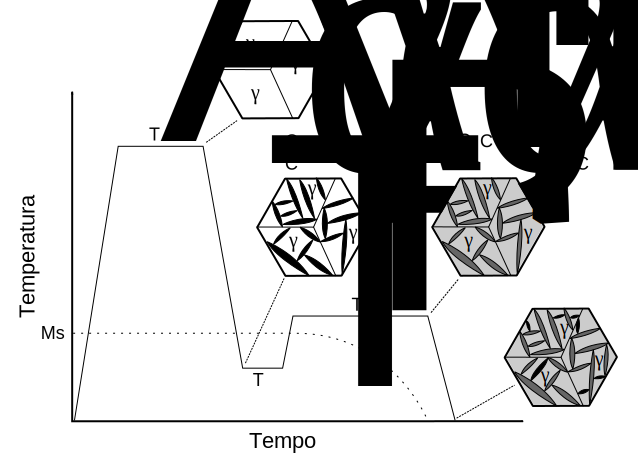
\includegraphics[width=.8\textwidth]{img/Q&P_steel.pdf}
  \end{figure}
\end{frame}

\begin{frame}{Introdução}
  % \only<1>{
  \begin{itemize}
    \item A partição de C de $\alpha'$ para $\gamma$ é termodinamicamente possível devido à diferença de potenciais químicos ($\mu_C^{\alpha'} > \mu_C^\gamma$)
    \item Speer propôs que $\mu_C^{\alpha'}$ e $\mu_C^\gamma$ se igualam após tratamento T\&P
    \item Equilíbrio Constrito de Carbono (ECC): $\mu_C^{\alpha'} = \mu_C^\gamma$  + interface $\alpha'/\gamma$ fixa
    % \item Os teores de C em $\alpha'$ e $\gamma$ são definidos a partir de $\mu_C^{\alpha'} = \mu_C^\gamma$ e das frações iniciais de $\alpha'$ e $\gamma$: Equilíbrio Constrito de Carbono (ECC)
    % \item Assim, C em $\alpha'$ e $\gamma$ depende da fração inicial de $\alpha'$ (depende de $T_T$)
  \end{itemize}

  \begin{figure}
    \includegraphics[width=.7\textwidth]{img/common_tangent_CCE.pdf}
  \end{figure}
  % }
  % \only<2>{
  %   \begin{figure}
  %     \includegraphics[width=.9\textwidth]{img/CCE_scheme.pdf}
  %   \end{figure}
  % }
\end{frame}

% \begin{frame}
%   \begin{itemize}
%     \item Neste trabalho, a evolução microestrutural e cinética durante a aplicação do processo de \textbf{Têmpera e Partição}\footnotemark[1] (T\&P) de um ferro fundido nodular foi estudada.
%     \item Esta microestrutura promete oferecer propriedades análogas às obtidas durante a transformação bainítica interrompida e aços TRIP e no ferro fundido nodular austemperado (ADI)
%   \end{itemize}
% \end{frame}

%\begin{frame}{Introdução}{Modelo termodinâmico aplicado ao T\&P}
  %\begin{itemize}
    %\item Modelo de Speer (2003): interface $\alpha'$:$\gamma$ imóvel e eq. apenas entre os átomos de C (Equilíbrio Restringido de Carbono - ERC)
    %\item Com base neste modelo, possível determinar \textbf{Temperatura de Têmpera} ótima TO que fornece maior quantidade de austenita
    %\item TT > TO: pouca $\alpha'$ formada, menos carbono para partição para $\gamma$; martensita fresca
    %\item TT < TO: $\gamma$ estabilizado à temperatura ambiente; quantidades menores de $\gamma$ pois é consumido pela formação de $\alpha'$ na têmpera
  %\end{itemize}
%
  %\begin{figure}
  %\includegraphics[height=5cm]{../texto/img/TPprevisto.pdf}
  %\end{figure}
%\end{frame}

\begin{frame}{Introdução}
  \begin{block}{Speer, 2004\footnotemark[1]}
    \begin{itemize}
    \item Speer propôs que o elevado teor de Si utilizado na elaboração de ferros fundidos os faria candidatos ótimos para serem submetido à rota T\&P, produzindo microestruturas semelhantes à dos \textbf{ferros fundidos austemperados} (ADI)
    \item Alunos de graduação da Colorado School of Mines, orientados por Speer, submeteram um ferro fundido nodular à rota T\&P e determinaram que o enriquecimento em C de $\gamma$ foi semelhante ao ADI, mas sua retenção foi significativamente menor
    \end{itemize}
  \end{block}

  % \begin{figure}
  % \includegraphics[height=3.8cm]{img/Speer2004.pdf}
  % \end{figure}

  \footnotetext[1]{Speer JG, Edmonds D V., Rizzo FC, Matlock DK. Curr Opin Solid State Mater Sci 2004;8:219.}
\end{frame}

\begin{frame}{Introdução}

  \begin{block}{Dissertação de Anderson J. S. T. Silva\footnotemark[1]}
    \begin{itemize}
    \item Duas ligas comerciais de ferro fundido nodular com alto manganês (> 0,5\%) $\rightarrow$ intensa segregação para contornos de célula eutética
    \item T\&P para diferentes tempos e temperaturas de partição; $T_T$ fixo
    \item Microestrutura composta de $\alpha'$ particionada e grandes quantidades de \textbf{ausferrita} (ferrita bainítica [$\alpha_b$] + $\gamma$), mesmo microconstituinte obtido no ADI
    \item Identificação de \textbf{janela de processo} similar ao ADI, cujo fim é associado ao 2º estágio da reação bainítica
    \end{itemize}

    % \begin{figure}
    %   \includegraphics[height=.3\textwidth]{img/MEV_Anderson.pdf}
    % \end{figure}
  \end{block}

  \footnotetext[1]{Silva AJST. Têmpera E Partição de Ferros Fundidos Nodulares. Dissertação (Mestrado). EPUSP, 2013.}
\end{frame}

\begin{frame}{Objetivos}
  Esse trabalho faz parte de um projeto maior que objetiva:
  \begin{enumerate}
    \item Demonstrar a viabilidade da rota T\&P aplicada a ferros fundidos (dissertação de mestrado de Anderson J. S. T. Silva, 2013)
    \item \textbf{Compreender as transformações de fases envolvidas, o entendimento de suas respectivas cinéticas e microestruturas obtidas (presente trabalho)}
    \item Medir as propriedades mecânicas do produto (tese doutorado de André Caetano Melado)
  \end{enumerate}
\end{frame}

% \begin{frame}{Objetivos}
%   \begin{enumerate}
%     \item Avaliar o efeito das variáveis de tratamento térmico na microestrutura final
%     \item Caracterizar a cinética da redistribuição de carbono durante a etapa de partição
%     \item Identificar e caracterizar as reações competitivas que podem ocorrer durante o tratamento de partição, como a reação bainítica e a precipitação de carbonetos
%     \item Avaliar o efeito da microssegregação de elementos de liga, inerente a produtos fundidos, na microestrutura final
%     \item Desenvolver um modelo para a cinética local de redistribuição de carbono durante a etapa de partição, considerando o efeito das reações competitivas.
%   \end{enumerate}
% \end{frame}

% %ADI

% %Equilíbrio Restringido de Carbono


\chapter{Objetivos}

Neste trabalho um ferro fundido nodular foi tratado termicamente segundo a rota de Têmpera e Partição. Isto é justificado pelo extenso conhecimento --- tanto científico, quanto tecnológico --- existente sobre o ferro fundido nodular austemperado (ADI), um material que se beneficia de uma mesma mistura de austenita estabilizada por carbono e ferrita acicular, obtida neste caso pela interrupção da reação bainítica. Neste sentido, o ferro fundido nodular temperado e particionado tem o potencial de substituir o ADI em uma quantidade de aplicações industriais.

O presente trabalho tem como objetivo caracterizar os microconstituintes presentes em um ferro fundido nodular submetida ao processo de Têmpera e Partição. Derivam do objetivo principal:

\begin{enumerate}
\item O estudo do efeito da intensa segregação presente em ferros fundidos na microestrutura final; 
\item A identificação de reações competitivas durante o tratamento de partição, como a reação bainítica e a precipitação de carbonetos;
%\item A investigação da ocorrência de transformação martensítica isotérmica em tratamentos próximos à temperatura Ms; 
\end{enumerate}


\chapter{Revisão Bibliográfica}

Este capítulo de revisão bibliográfica está estruturado em quatro seções principais que contextualizam os objetivos do presente trabalho. A seção \ref{sec:Fofos} fornece uma descrição, com enfoque nas transformações de fases, do atual conhecimento sobre o material estudado neste trabalho, o ferro fundido nodular. Nesta seção também são apresentados dois importantes assuntos utilizados na discussão dos resultados deste trabalho, a microsegregação de elementos de liga durante a solidificação do metal e a interrupção da reação bainítica para produção de microestruturas compostas de ferrita e austenita estabilizada por enriquecimento em carbono.

Na seção \ref{sec:consTransf} são expostos conceitos sobre controle cinético de transformações difusionais, utilizados no modelo termodinâmico para predição das microestruturas produzidas pelo processo de Têmpera e Partição (T\&P). Na seção seguinte, é apresentada uma descrição sobre a transformação martensítica em ligas ferrosas baseada no entendimento consolidado sobre esta reação. Procurou-se omitir aspectos sobre a cristalografia da transformação e a discussão sobre o mecanismo da reação bainítica, ainda alvo de controvérsia.

Por fim, na seção \ref{sec:processoTP} é apresentada a revisão bibliográfica sobre o processo de Têmpera e Partição, enfatizando os trabalhos exploratórios do grupo da \enfase{Colorado School of Mines} no início da década de 2000 e o modelo termodinâmico desenvolvido por Speer e colaboradores \cite{Speer2003}. Também foi incluída nesta seção uma revisão sobre transformações que podem ocorrer competitivamente durante a etapa de partição do processo T\&P.

\section{Ferros fundidos nodulares}

\label{sec:Fofos}

Os ferros fundidos, de forma simplificada, podem ser considerados ligas ternárias Fe-C-Si, contendo também teores de impurezas (Mn, P e S) e de elementos adicionados intencionalmente como agentes modificadores (Mg e Ce). Sua solidificação apresenta uma fase pró-eutética (austenita ou grafita), completada por uma reação de solidificação eutética, que pode ser estável ($\text{líquido} \rightarrow \text{austenita} + \text{grafita}$), ou metaestável ($\text{líquido} \rightarrow \text{austenita} + \text{cementita}$).

Ferros fundidos nodulares correspondem a uma classe dos ferros fundidos em que a morfologia da grafita é apresentada na forma de nódulos esferoidizados, estrutura conseguida por meio da adição de elementos químicos modificadores, sendo o Mg e o Ce os mais comuns.

A grafita é formada pelo empilhamento de camadas planas constituídas de átomos de carbono ligados covalentemente na forma de uma estrutura hexagonal. Durante a solidificação, a grafita pode crescer na direção dos planos basais ou dos planos prismáticos (vide figura \ref{fig:grafita}), assumindo a forma de lamelas ou esferas em função da composição química e do processamento do metal líquido. Elementos tensoativos, como oxigênio e enxofre, tendem a ser adsorvidos pelos planos prismáticos da célula da grafita, diminuindo a energia interfacial destas superfícies e, portanto, favorecendo o crescimento da fase nestas direções, resultando em morfologias lamelares. Na ausência destas impurezas, o crescimento nos planos prismáticos não é favorecido e, em consequência, a grafita preponderantemente na direção dos planos basais, adquirindo a morfologia de glóbulos esféricos. A utilização de magnésio no tratamento pré-vazamento do metal líquido visa a eliminação das impurezas e a obtenção de grafita nodular, uma vez que o Mg possui forte ação desoxidante e dessulfurante\cite{Labrecque1998,Guesser2009}.

\begin{figure}
	\includegraphics[width=10cm]{img/grafita.pdf}
	\caption{Esquema de crescimento da grafita nas direções normais aos planos basais e prismáticos\cite{Guesser2009}.}
	\label{fig:grafita}
\end{figure}

É comum a prática de inoculação do ferro fundido com elementos de ação grafitizante, pouco antes de seu vazamento, com o objetivo diminuir o super-resfriamento para o início da formação da grafita e, assim, evitar que o eutético metaestável seja formado\cite{Santos1991}. O grau de inoculação de ferros fundidos nodulares controla a dispersão dos nódulos de grafita no metal e, consequentemente, também o espaçamento entre as células eutéticas.

\subsection{Solidifica\c{c}\~{a}o}

A solidificação dos ferros fundidos nodulares é descrita de acordo com as reações dos eutéticos estável $\text{líquido} \rightarrow \text{austenita} + \text{grafita}$. A composição química e a velocidade de resfriamento são os principais parâmetros que definem a natureza da reação eutética nos ferros fundidos. Enquanto no sistema Fe-C a diferença entre as temperaturas de equilíbrio do eutético estável e metaestável é de aproximadamente 7 °C, ligas contendo 2\% em massa de silício tem essa faixa ampliada para 35 °C\cite{Santos1991}. O silício e outros elementos que possuem a propriedade de aumentar a diferença entre os dois eutéticos, como o alumínio, níquel e cobre, são chamados de elementos grafitizantes. Por outro lado, elementos que são fortes formadores de carbonetos, como o cromo, vanádio e o tungstênio tendem a aproximar os dois eutéticos. Por esta propriedade, são geralmente empregados na produção de ferros fundidos brancos. Altas taxas de resfriamento favorecem a formação do eutético metaestável, uma vez que a formação da cementita é mais rápida do que a precipitação da grafita.

Em ferros nodulares de composição eutética, a solidificação se inicia após a aplicação de um super-resfria-%atentar a essa quebra de linha
mento ao líquido a temperaturas inferiores à do eutético estável, quando se dá a nucleação e crescimento dos nódulos de grafita. Na sequência, os nódulos formados são encapsulados por um invólucro de austenita, formando a denominada célula eutética. As células eutéticas continuam crescendo até que todo o calor latente da solidificação seja liberado e a solidificação tenha chegado a seu fim\cite{Santos1991}. %Vide\cite{Stefanescu2005} para citar Patterson e Scheil (1949)

A reação eutética no ferro fundido nodular apresenta uma característica que o difere, por exemplo, da reação eutética em um ferro fundido cinzento. Neste último caso, os dois produtos da reação, austenita e grafita de morfologia lamelar, se formam simultaneamente. No ferro fundido nodular a formação da austenita e da grafita ocorre em momentos distintos. O constituinte eutético é, portanto, do tipo ``divorciado'', em contraste ao crescimento cooperativo observado na reação eutética de ferros cinzentos\cite{Santos1991}.

Em ligas hipoeutéticas e hipereutéticas, por sua vez, há a formação de uma fase primária no início da solidificação. No primeiro caso, a solidificação se inicia com a formação de dendritas de austenita, enquanto no segundo caso nódulos de grafita são formados diretamente a partir do líquido. Em ambos os casos, na medida em que o material é resfriado, a composição do líquido progressivamente se aproxima da composição eutética. A reação eutética, no entanto, só se inicia uma vez atingido um super-resfriamento suficiente para nucleação e crescimento dos nódulos de grafita\cite{Santos1991}.

Na microestrutura final das ligas eutética e hipoeutética é normalmente observada uma população de nódulos de grafita com tamanhos dispersos segundo uma distribuição Gaussiana. Em ligas hipereutéticas, por sua vez, são observadas duas diferentes populações de nódulos de grafita: uma cuja média dos diâmetros é maior, correspondente aos nódulos formados entre a temperatura \enfase{liquidus} e a temperatura do eutético metaestável, e outra cujo tamanho médio da população é menor, formada durante a reação eutética\cite{Santos1991}. %citar quem o Santos cita

\subsubsection{Microsegrega\c{c}\~{a}o de elementos durante a solidifica\c{c}\~{a}o}

Microsegregação é o termo que define a condição de não-uniformidade de composição química no material a nível microestrutural. Em complemento à definição de microsegregação, macrosegregação trata-se da não-uniformidade de composição química em larga escala, comparável ao tamanho da peça. A macrosegregação é um defeito do processo de fundição do metal e, portanto, seu controle possui caráter tecnológico. Por outro lado, a microsegregação é inerente ao produto fundido e, dessa forma, tem sua devida importância reconhecida nesta seção do texto.

A microsegregação se origina devido à expulsão de soluto da fase sólida ao crescer a partir do metal líquido. Caso a liga seja resfriada lentamente, o contato prolongado entre líquido e sólido permitirá a difusão de soluto até o estabelecimento do equilíbrio termodinâmico para cada temperatura; esta construção hipotética leva à elaboração dos diagramas de fase. No entanto, nas situações reais, em que taxas de resfriamento elevadas são impostas ao material, a rejeição do soluto da fase sólida para a fase líquida estabelece uma heterogeneidade de composição ao final da solidificação. Dessa forma, na microestrutura bruta de fundição há a preponderância do soluto nas últimas porções de metal a se solidificar.

Em ferros fundidos a microsegregação também é originada na formação da fase de solidificação primária, mas é principalmente atribuída à reação eutética. Como estas ligas possuem ao menos três elementos químicos, a regra das fases de Gibbs\footnotemark prevê que a reação eutética $\text{líquido} \rightarrow \text{austenita} + \text{grafita}$ não ocorre em um ponto invariante, mas sim em uma faixa de temperaturas. Devido às limitadas difusividades dos elementos na fase sólida e à dependência de suas solubilidades no líquido em função da temperatura de solidificação, ocorre que as sucessivas camadas de austenita formadas a partir do líquido apresentam diferentes composições químicas. Assim, elementos que apresentam maior solubilidade na austenita em temperaturas mais elevadas, como silício, níquel e cobre, tendem a se concentrar nas primeiras regiões a se solidificar. Na formação do eutético divorciado do ferro nodular, portanto, estes elementos se concentrarem próximos aos nódulos de grafita. Por outro lado, carbono, enxofre, manganês, cromo e molibdênio são rejeitados da austenita para líquido e acabam permanecendo em maior concentração nas últimas regiões a se solidificar, isto é, aquelas que correspondem ao encontro das células eutéticas. %Referenciar e inserir figura

\footnotetext{A regra das fases foi proposta por J.W. Gibbs em seu famoso trabalho de 1878 \enfase{On the Equilibrium of Heterogeneous Substances}\cite{Gibbs1878}. A equação estabelece a igualdade $F = C - P + 2$, em que $F$ é o número de graus de liberdade (número de variáveis de estado independentes), $C$ o número de componentes do sistema e $P$ o número de fases. Para um sistema constituído apenas de fases condensadas, em que o efeito da pressão é desprezível, pode ser simplificado para $F = C - P + 1$.}

Uma ferramenta muito útil para o entendimento e quantificação (estimativa) da microsegregação é o modelo de Scheil-Gulliver. %\cite{Porter2009}
A equação desenvolvida por Scheil apud \citaremsentenca{Porter2009} %pegar referência original do Scheil?
vale para uma liga binária cuja solidificação gera apenas uma fase sólida. As hipóteses de Scheil representam a situação de máxima segregação, em que a difusão do soluto na fase sólida é completamente desprezada e, portanto, não é possível o estabelecimento do equilíbrio termodinâmico em todo o sistema. As considerações feitas neste modelo são\cite{Porter2009}:

\begin{enumerate}
	\item Não há difusão na fase sólida após sua formação;
	\item A difusão é infinitamente rápida na fase líquida para todas as temperaturas. Essa ponderação é equivalente a considerar a composição química homogênea ao longo de todo o líquido;
	\item As composições na interface sólido-líquido são de equilíbrio, valendo as composições preditas pelo diagrama de fases em uma dada temperatura. Essa hipótese não significa que há o estabelecimento do equilíbrio no sistema, mas \enfase{apenas} na interface. Ela é semelhante à adotada por Zener para transformações difusionais em estado sólido (vide seção \ref{sec:consTransf});
	\item As linhas \enfase{solidus} e \enfase{liquidus} são representadas por linhas retas no diagrama de fases. \label{item:scheil4}
\end{enumerate}

Postas estas condições, define-se o coeficiente de partição $k$, que corresponde à razão entre o teor de soluto $C_S$ na fase sólida a composição química $C_L$ na fase líquida, ambas consultadas no diagrama de fases:

\begin{subequations}
	\begin{align}
		\label{eq:coefPart}k = \frac{C_S}{C_L}
	\end{align}
\end{subequations}

Note-se que, devido à hipótese \ref{item:scheil4}, $k$ assume valor constante. Atualmente, graças ao aumento do poder computacional e ao desenvolvimento de bases de dados termodinâmicos, esta hipótese pode ser relaxada utilizando técnicas numéricas, tais quais as empregadas nos pacotes de software que empregam o método CALPHAD. %pacote de software? protocolo? não sei direito o que é o CALPHAD

\novasiglaestrangeira{CALPHAD}{Computer Coupling of Phase Diagrams and Thermochemistry} %Prestar atenção se fica dentro ou fora da ordem alfabética.

As demais equações que definem o problema consistem da condição inicial de solidificação (equação \ref{eq:condIni}), isto é, que a composição do líquido no início da solidificação é igual à composição média da liga $C_0$, a conservação de massa do sistema (equação \ref{eq:balSis}), dada pela soma unitária das frações de sólido ($f_S$) e líquido ($f_L$), e o balanço de massa na interface (equação \ref{eq:Stefan}), que corresponde ao balanço entre a redistribuição do soluto e o aumento da fração de sólido.

\begin{subequations}[resume]
	\begin{align}
		\label{eq:condIni}\left.C_L\right|_{f_S=0} &= C_0\\
		\label{eq:balSis}f_S + f_L &= 1\\
		\label{eq:Stefan}\left(C_L - C_S\right) df_S &= f_L dC_L
	\end{align}
\end{subequations}

A integração da equação diferencial \ref{eq:Stefan} nos domínios de integração definidos pela condição inicial (equação \ref{eq:condIni}) utilizando as substituições dos termos adequados obtidos pelas equações \ref{eq:coefPart} e \ref{eq:balSis} leva à equação de Scheil-Gulliver para composição do sólido e do líquido durante a solidificação:

\begin{subequations}
	\begin{align}
		C_L &= C_0 {f_L}^{k-1}\\
		\label{eq:C_S}C_S &= k C_0\left(1 - f_S\right)^{k-1}
	\end{align}
\end{subequations}

Graças ao desenvolvimento de bases de dados termodinâmicas é possível também utilizar as considerações de Scheil para estimar a microsegregação durante a solidificação de ligas multicomponentes, que frequentemente geram mais de uma fase sólida diretamente do líquido. Softwares que seguem o método CALPHAD, como o Thermo-Calc\textregistered, possuem módulos que permitem esse tipo de contabilização. Adicionalmente, quando acoplados com informações sobre a difusividade dos elementos químicos, também permitem a utilização de condições de equilíbrio parcial na interface (tal quais as apresentadas na seção \ref{sec:consTransf}) e aplicação de difusão no estado sólido\cite{Chen2002,Larouche2007}.

\subsection{Transforma\c{c}\~{o}es no estado s\'{o}lido}

Durante o resfriamento lento do metal solidificado, em torno de 720 °C ocorre a decomposição eutetóide da austenita, que, assim como a reação eutética, pode acontecer na forma estável ($\text{austenita} \rightarrow \text{ferrita} + \text{grafita}$) ou metaestável ($\text{austenita} \rightarrow \text{ferrita} + \text{cementita}$). A predominância de uma reação ou outra é novamente dependente da taxa de resfriamento e da composição química.

Durante a reação do eutetóide estável, a austenita se decompõe em ferrita e grafita secundária. A nucleação da ferrita se dá preferencialmente na interface entre a austenita e os nódulos de grafita formados durante a solidificação. A ferrita cresce para o interior da austenita, enquanto a grafita é incorporada aos nódulos pré-existentes. Em estágios avançados da reação a ferrita engloba completamente o nódulo, formando uma barreira para a difusão de carbono da austenita para a grafita, diminuindo substancialmente a velocidade da reação. A tendência a partir desse ponto é que a reação do eutetóide metaestável, que corresponde à decomposição da austenita em perlita, predomine e consuma a austenita não-transformada. A figura \ref{matrizFofo} ilustra a sequência de etapas da decomposição eutetóide da austenita.

\begin{figure}
	\includegraphics[width=10cm]{img/matrizFofo.pdf}
	\caption{Ilustração esquematizando a decomposição eutetóide em ferros fundidos nodulares\cite{Johnson1978}.}
	\label{matrizFofo}
\end{figure}

A perlita consiste de um agregado de lamelas alternadas de ferrita e cementita. O crescimento da perlita se dá de forma cooperativa, ou seja, as duas fases crescem simultaneamente. Ao contrário da precipitação de grafita no estado sólido, a formação de cementita não carece da difusão a longo alcance dos átomos de Fe. Por este motivo, para uma ampla faixa de temperaturas a cinética da reação perlítica é consideravelmente mais rápida do que a formação do eutetóide estável. \citaremsentenca{Zener1946} estudou a cinética local de crescimento da perlita assumindo que a distância de difusão característica de seu crescimento seria o espaçamento interlamelar. Em consequência, Zener concluiu que a velocidade de crescimento de uma colônia é constante e independente da porção transformada da austenita, ao contrário do que acontece no eutetóide estável.

Elementos como antimônio, cobre e estanho são chamados de ``perlitizantes'' por atuarem evitando a formação da ferrita oriunda do eutetóide estável\cite{Kovacs1981}.
A obtenção de uma matriz perlítica também pode ser conseguida por meio de tratamentos térmicos, como é o caso da normalização. Matrizes completamente ferríticas também podem ser obtidas por meio tratamentos térmicos. O recozimento é um tratamento térmico em que a peça é aquecida a temperaturas próximas à de início de eutetóide estável que leva à dissociação da perlita para formação da estrutura de equilíbrio ferrita + grafita\cite{Guesser2009}.

Além das matrizes ferrítica e perlítica convencionais, ferros fundidos podem ser submetidos a tratamentos de têmpera, para obtenção de uma matriz martensítica, e austêmpera, para obtenção de matriz constituída de bainita isenta de carbonetos e austenita retida estabilizada por carbono. Estas matrizes conferem ao material resistência mecânica muito superiores às matrizes ferrítica e perlítica e, no caso do produto austemperado, elevadas ductilidade e tenacidade ao impacto\cite{Guesser2009}.

\subsection{Ferro fundido nodular austemperado (ADI)}

\label{subsec:ADI}

Em aços carbono, tratamentos isotérmicos aplicados à austenita em temperaturas inferiores às de formação da perlita geram um microconstituinte eutetóide denominado bainita. Morfologicamente, a bainita se apresenta na forma de ripas de ferrita (ou agulhas, como é visto em uma seção bidimensional) contendo carbonetos dispersos ou entre cada unidade de ferrita (bainita superior), ou em seu interior (bainita inferior).

Em ligas ferrosas contendo silício a transformação bainítica possui uma cinética característica, consistindo de uma etapa inicial de formação de feixes de ferrita pró-bainítica, prosseguida por um período de estagnação conhecido como ``estase'', para que a reação, enfim, possa ser retomada pela precipitação de carbonetos nas ilhas de austentita não-transformadas\cite{Goldenstein2002}. Durante a primeira etapa da reação nestas ligas, a ferrita bainítica progressivamente enriquece em carbono a austenita adjacente. Como será discutido na seção \ref{sec:Martensita} deste trabalho, austenita com teores elevados carbono possui pouca tendência de se transformar durante o resfriamento. Assim, dependendo do teor médio de carbono da liga, se a reação é interrompida durante a estase, uma grande quantidade de austenita estabilizada em carbono pode ser retida na temperatura ambiente.

O ferro fundido nodular austemperado (do inglês, \siglaestrangeira{ADI}{Austempered Ductile Iron}) faz uso desse fenômeno para obtenção de uma matriz bifásica de finas ripas de ferrita intercaladas com filmes de austenita --- produto chamado de ``ausferrita'' na literatura de fundição. Nos ferros fundidos o fenômeno da estase é prologando devido aos elevados teores de silício inerentes a esse material. Ainda assim, o processo é somente viável em uma ``janela de processo'', que corresponde ao intervalo de tempos e temperaturas em que o produto austemperado confere propriedades dentro das faixas de propriedades estabelecidas pela norma ASTM A897\cite{Bayati1999,ASTMA8972006} e normalmente termina com a precipitação de carbonetos na reação bainítica. Quando produzida nos parâmetros adequados de tratamento térmico, a ausferrita confere ao ADI elevada resistência mecânica aliada a elevada ductilidade devido à ocorrência do efeito TRIP (\enfase{Transformation Induced Plasticity})\cite{Goldenstein2002}. Por este motivo, o ADI proporciona propriedades comparáveis às obtidas em aços, em algumas situações se mostrando favoravelmente competitivo por agregar as vantagens de produção próxima da forma final (\enfase{near-net-shape}) decorrente do processo de fundição\cite{Trudel1997,Hayrynen2002}.

O tratamento térmico para produção do ADI, ilustrado na figura \ref{fig:austempera}, consiste de uma etapa inicial de aquecimento até o campo de equilíbrio entre austenita e grafita (austenitização), na qual o material é mantido durante um determinado tempo de encharque. Em seguida, as peças são mergulhadas em banho de sal fundido, pré-aquecido na temperatura de austêmpera, onde são mantidas por tempo suficiente para que a austenita enriquecida em carbono seja retida à temperatura ambiente\cite{Trudel1997}.

\begin{figure}
	\includegraphics[height=10cm]{img/austemperaTTT_Meier.pdf}
	\caption{Diagrama TTT esquemático ilustrando o processo de austêmpera de ferros fundidos\cite{Meier2013a}.}
	\label{fig:austempera}
\end{figure}

A temperatura de austenitização controla a composição da austenita em equilíbrio com a grafita. Temperaturas mais elevadas ajudam na redistribuição do manganês segregado para os contornos de célula eutética e atribuem um maior teor de carbono à austenita, conferindo, portanto, também maior temperabilidade ao material. Nesse caso, tempos mais prolongados de austêmpera seriam necessários para o início da transformação bainítica e, uma vez estabelecido o final da primeira etapa da reação, maiores frações de austenita retida acabam por ser obtidas. A elevada temperabilidade também confere menor tendência de formação de perlita durante o resfriamento, indesejável para o alcance das propriedades mecânicas\cite{Trudel1997}. O uso intensivo de elementos químicos produz efeito semelhante sobre a temperabilidade do material, mas deve ser utilizado com especial cuidado devido aos problemas associados à microsegregação\cite{Bayati1995,Velez1996}.

\citaremsentenca{Trudel1997} apontam que o tempo de austenitização deve ser o mínimo possível para que garantir que o material se transforme completamente em austenita saturada em carbono e grafita, sendo o tempo de uma hora à temperatura de 900 °C em uma peça de 25 mm de diâmetro geralmente suficiente para garantir isso. No entanto, para temperaturas mais baixas, tempos superiores a três horas podem ser necessários para a eliminação das heterogeneidades de composição química.

A temperatura de austêmpera desempenha o papel mais importante no estabelecimento das propriedades mecânicas do ADI. Temperaturas elevadas levam à formação de um produto com excelente ductilidade e resistência a esforços dinâmicos, enquanto temperaturas baixas geram um produto extremamente resistente e resistência ao desgaste\cite{Lin1996,Aranzabal1997,Magalhaes1998}. Microestruturalmente, a ausferrita formada em duas temperaturas diferentes apresenta mudanças significativas. Como pode ser observado na figura \ref{fig:ADIs}a, o material tratado termicamente a 360 °C apresenta ripas grosseiras de bainita com grandes quantidades de austenita, enquanto ADI produzido a 310 °C possui uma microestrutura mais refinada, composta de menores ilhas de austenita isoladas umas das outras.

\begin{figure}
	\subfloat[]{\includegraphics[height=5.8cm]{img/ADI360oC.pdf}}
	\quad
	\subfloat[]{\includegraphics[height=5.8cm]{img/ADI310oC.pdf}}
	\caption{Microestruturas de ADIs produzidos pela austêmpera a (a) 360 °C e (b) 310 °C por uma hora. Imagens reproduzidas de\cite{Trudel1997}.}
	\label{fig:ADIs}
\end{figure}

Um aspecto importante da produção do ADI é o efeito da microsegregação na transformação bainítica no material. Como mencionado anteriormente, alguns autores reportam que é conveniente eliminar a microsegregação durante a etapa de austenitização. A justificativa para aplicação de tal medida é ilustrada na figura \ref{fig:cineticaADI}, que mostra esquematicamente o crescimento das colônias de ausferrita no ferro fundido. Devido à segregação nos contornos de células eutéticas, estas regiões possuem maior temperabilidade e, consequentemente, apresentam uma cinética mais lenta de transformação. \citaremsentenca{Trudel1997} reportam que estas regiões, por não se transformarem, devem estar empobrecidas em carbono e, dessa forma, embora já estejam enriquecidas por elementos que auxiliam na retenção da austenita, podem não reter totalmente a austenita na temperatura ambiente, se transformado parcialmente em martensita. \citaremsentenca{Bayati1995} mostraram que em um ferro nodular contendo 0,67\% de manganês, devido à diferença entre as cinéticas de transformação nas duas regiões, ocorre a superposição das etapas de transformação da ausferrita. Isto é, enquanto as regiões intercelulares ainda estão enriquecendo a austenita em carbono no primeiro estágio da reação, nas primeiras regiões a se transformar a precipitação de carbonetos já se iniciara. Este fenômeno leva à diminuição da janela de processo do material. \citaremsentenca{Meier2013a} fizeram observações semelhantes por meio de difração de nêutrons \enfase{in situ} e mostraram que a formação da ausferrita é associada a uma assimetria dos picos de difração da austenita, atribuída a fases com cinéticas de transformação diferentes.

\begin{figure}
	\includegraphics[width=16cm]{img/crescimentoAusferrita.pdf}
	\caption{Esquema representando, de forma simplificada, a evolução da formação de ausferrita em um ADI. A região hachurada corresponde à estrutura de ferrita bainítica entremeada por filmes de austenita enriquecida em carbono. As últimas poças não-trasformadas de austenita geralmente correspondem a contornos de célula eutética. Extraído de\cite{Aranzabal1997}.}
	\label{fig:cineticaADI}
\end{figure}


\section{Considera\c{c}\~{o}es sobre transforma\c{c}\~{o}es difusionais em ligas multicomponentes}

\label{sec:consTransf}

O atual desenvolvimento das teorias cinéticas de crescimento difusional de fases é em grande parte creditado ao trabalho pioneiro de \citaremsentenca{Zener1946}. Zener construiu um modelo cinético para o crescimento da ferrita a partir da austenita no sistema Fe-C. Para tanto, supôs que as composições na interface entre matriz e precipitado seriam dadas pelas linhas de solubilidade do diagrama de equilíbrio do sistema. Um tratamento mais completo necessita levar em conta vários elementos de liga, o que implica em um grande aumento de complexidade do problema no ponto de vista de modelamento do fenômeno. Particularmente, quando há a adição de elementos substitucionais, a diferença de mobilidade entre os solutos intersticial e substitucionais acarreta em situações de controle cinético com diferentes características, dependendo das forças motrizes às quais o material está sendo submetido. Assim, dependendo da velocidade da movimentação da interface, convém-se classificar as condições interfaciais em dois diferentes modos: equilíbrio local e paraequilíbrio.

\subsection{Equilíbrio local (EL)}
	
\novasigla{EL}{Equilíbrio local}

A condição de equilíbrio local é caracterizada pela movimentação lenta da interface, de modo a permitir que o equilíbrio local na interface entre precipitado e matriz seja estabelecido. Trata-se da situação assumida por Zener, em a igualdade dos potenciais químicos dos elementos na interface entre as duas fases é obedecida. A condição termodinâmica de EL no crescimento de ferrita ($\alpha$) a partir da austenita ($\gamma$) é dada por:

\begin{equation}
	\mu_i^\alpha = \mu_i^\gamma
\end{equation}
%
em que $\mu_i$ é o potencial químico do elemento $i$ (= C, Mn, Si, Cr, etc) na fase.

No que lhe diz respeito, ainda é possível discernir duas situações de EL, dependendo de como os solutos substitucionais são redistribuídos entre a fase em crescimento e a fase matriz.

Sob baixos super-resfriamentos, ocorre considerável redistribuição dos elementos substitucionais entre as duas fases. Nesta situação, conhecida como equilíbrio local com partição de soluto (EL-P)\novasigla{EL-P}{Equilíbrio local com partição de soluto}, a difusão dos substitucionais, por ser mais lenta do que a difusão dos elementos intersticiais, controla a movimentação da interface. Os perfis de composição na interface para a condição EL-P são mostrados na figura \ref{fig:modcineticos}a.

Sob forças motrizes maiores, a redistribuição do soluto substitucional entre as duas fases é mínima. Neste cenário, chamado de equilíbrio local com partição desprezível de soluto\novasigla{EL-PD}{Equilíbrio local com partição desprezível de soluto}, a composição das fases fora das redondezas da interface é praticamente a mesma. Por sua vez, nas proximidades da interface há a formação de uma ``crista'' (\enfase{spike}) de concentração de soluto (vide figura \ref{fig:modcineticos}b), de modo que as condições de equilíbrio sejam estabelecidas na interface e, portanto, a difusão do elemento intersticial controla a cinética da reação. Nesta condição, portanto, a movimentação da interface tende a ser mais rápida do que na situação de EL-P. %Não esquecer de pegar e citar artigos de Popov e Mikhalev, Darken, Kirkaldy e Hillert.\cite{Darken1961}\cite{Hillert1968}

\begin{figure}
	\subfloat[]{\includegraphics[height=5.8cm]{img/EL-P.pdf}}
	\hspace{1.5cm}
	\subfloat[]{\includegraphics[height=5.8cm]{img/EL-PD.pdf}}
	\vspace{0pt}
	\subfloat[]{\includegraphics[height=5.8cm]{img/PE.pdf}}
	\caption{Perfis de composição ($x_C$) e fração de sítios substitucionais ($y_j$) na ferrita ($\alpha$) e na austenita ($\gamma$) segundo os modelos cinéticos de (a) equilíbrio local com partição de soluto (EL-P); (b) equilíbrio local com partição desprezível de soluto (EL-PD); e (c) paraequilíbrio (PE).}
	\label{fig:modcineticos}
\end{figure}

\subsection{Paraequilíbrio (PE)}

\novasigla{PE}{Paraequilíbrio}

\citaremsentenca{Hultgren1947} observou que, durante a decomposição eutetóide da austenita em ferrita e cementita, o produto formado usualmente herdava a mesma composição de elementos substitucionais da fase matriz. Ele chamou estes produtos de paraferrita e paracementita, em oposição às fases de equilíbrio pleno. Em adição, Hultgren argumentou que o crescimento destas \enfase{parafases} ocorreria segundo uma condição termodinâmica específica, denominada paraequilíbrio, na qual duas fases estariam em equilíbrio real uma em relação à outra apenas com respeito aos componentes de maior mobilidade, ou seja, os elementos intersticiais.

A situação de paraequilíbrio ocorre devido à grande diferença de mobilidade entre os solutos substitucionais e o soluto intersticial. Esta situação é passível de ocorrer em baixas temperaturas, quando a difusão dos substitucionais é lenta\cite{Hillert1953}. Adicionalmente, se os elementos substitucionais são impedidos de se redistribuir, seus potenciais químicos individuais não podem ser igualados. Dessa maneira, o comportamento termodinâmico do sistema deve ser avaliado pelo potencial químico $\mu_Z$ do elemento hipotético $Z$\cite{Ghosh2001}, de modo a serem obedecidas as relações termodinâmicas que regem o paraequilíbrio:

\begin{subequations}
	\begin{align}
		\mu_C^\alpha &= \mu_C^\gamma \label{eq:potQuimC}\\
		y_j^\alpha &= y_j^\gamma \label{eq:fracSitios}\\
		\mu_Z^\alpha \left ( \equiv \sum y_j^\alpha \mu_j^\alpha \right) &= \mu_Z^\gamma \left ( \equiv \sum y_j^\gamma \mu_j^\gamma \right ) \label{eq:potQuimZ}
	\end{align}
\end{subequations}
%
em que $y_j$ são as frações de sítios substitucionais do elemento $j$ (= Mn, Si, Cr, Ni, etc.) nas fases matriz $\gamma$ e em crescimento $\alpha$. Note-se que o potencial químico do elemento teórico $Z$ é definido como a soma dos potenciais químicos dos elementos substitucionais ponderados pelas suas respectivas frações de sítios na fase. Por sua vez, para um sistema que contém tanto elementos substitucionais, quanto um elemento intersticial (no caso, o carbono), $y_j$ se correlaciona com a fração molar $x_j$ do substitucional na fase pela expressão:

\begin{equation}
	y_j = \frac{x_j}{1 - x_C}
\end{equation}
%
em que $x_C$ é a fração molar do carbono na fase.

A figura \ref{fig:modcineticos}c ilustra esquematicamente os perfis de composição no crescimento da ferrita a partir da austenita obedecendo as condições de paraequilíbrio. É importante ressaltar que, segundo a definição de Hultgren, tanto as fases formadas segundo o mecanismo de paraquilíbrio, quanto pelo mecanismo de equilíbrio local com partição desprezível de soluto são consideradas parafases. Na situação de EL-PD, embora as composições na interface obedeçam o equilíbrio pleno local, os teores médios de substitucionais em cada fase são praticamente os mesmos\cite{Hillert2004a}.


\section{Transforma\c{c}\~{a}o Martens\'{i}tica}

\label{sec:Martensita}

Nas ligas ferrosas contendo carbono, quando a decomposição eutetóide da austenita, controlada pela difusão dos elementos de liga, é evitada pelo rápido resfriamento do material a partir da temperatura de autenitização, a austenita tende a se decompor por um mecanismo não difusional na fase metáestável martensita. Nestas ligas a transformação martensítica normalmente gera uma fase de estrutura cristalina tetragonal de corpo centrado em temperaturas inferiores à temperatura de início da transformação martensítica (temperatura Ms). Em situações especiais é possível que uma martensita de estrutura hexagonal compacta se forme a partir da austenita. Outros sistemas de ligas também apresentam transformação do tipo martensítica, mas a importância tecnológica da martensita de ligas baseadas no elemento ferro supera todas as aplicações dos demais sistemas.

\simbolo{Ms}{Temperatura de início da transformação martensítica}

A transformação martensítica em aços carbono é acompanhada de expansão volumétrica do material, tal qual ocorre na formação da ferrita a partir da austenita. Como não há redistribuição de soluto entre as duas fases, o produto resultante herda a composição química da fase ancestral de austenita. A presença dos elementos químicos em solução sólida na martensita, em especial o carbono, desempenha papel crítico em seu endurecimento. A formação da martensita é acompanhada da ocupação de posições assimétricas nos sítios intersticiais octaédricos pelos átomos de carbono, fenômeno que leva ao estabelecimento da tetragonalidade da martensita\cite{Zener1946,Hillert1986}. Adicionalmente, a cristalografia da transformação martensítica requer que uma deformação cisalhante seja aplicada à célula unitária da austenita, como teorizado por Bain\cite{Bain1924}. Para compensar este cisalhamento, de modo que um plano invariante macroscópico seja mantido entre as duas fases, é necessário que a martensita recém formada sofra uma distorção para ser acomodada na austenita. Essa distorção é conhecida como deformação de plano invariante\cite{Honeycombe2006} e em magnitude é tão maior quando maior a tetragonalidade da martensita. Como ilustrado na figura \ref{fig:cisMartensita}, essa deformação pode ser obtida por meio do escorregamento de planos cristalinos e consequente criação de discordâncias no interior da fase, ou pela criação de defeitos de maclas na martensita.

\begin{figure}
	\includegraphics[width=14cm]{img/shearMartensite.pdf}
	\caption{Figura ilustrando que tanto (b) escorregamento quanto (c) maclação podem compensar o cisalhamento \textit{s} produzido pela deformação de Bain esquematizada em (a). No detalhe, imagens obtidas por microscopia eletrônica de transmissão das microestruturas dos dois tipos de martensita. Adaptado de\cite{Porter2009}.}
	\label{fig:cisMartensita}
\end{figure}

A tetragonalidade da martensita aumenta com fração de sítios intersticiais ocupados por átomos de carbono. Consequentemente, os defeitos cristalinos relacionados à deformação de plano invariante são mais extensos em ligas de alto carbono. Esse raciocínio leva à conclusão de que a martensita de médio e alto carbono possui elevada dureza, associada, porém, a valores muito baixos de alongamento. Por outro lado, a martensita formada em ligas de baixo carbono pode apresentar estrutura cristalina cúbica de corpo centrado após um certo período de envelhecimento. \citaremsentenca{Speich1972} pontuaram que este fenômeno se deve à segregação do carbono para discordâncias e contornos de ripas de martensita, sendo que o ponto de saturação dos defeitos cristalino ocorre em torno de 0,2\%C.

A natureza da deformação de plano invariante é utilizada para classificação da morfologia da martensita. Assim, a martensita acomodada pela formação de discordâncias e acionamento de planos de escorregamento é denominada martensita escorregada ou, em virtude de sua morfologia característica, martensita em ripas. Por sua vez, a martensita constituída de maclas é chamada de martensita maclada ou em placas. A predominância da ocorrência de uma morfologia ou outra está normalmente associada à composição química da austenita antecessora. Como mostra a figura \ref{fig:MsZhaoNotis}, dada uma composição fixa, a cada morfologia de martensita é associada uma temperatura Ms. O aumento do teor de carbono leva à diminuição simultânea das duas temperaturas Ms, mas esta tendência é maior para a martensita em ripas. Assim, teores de carbono mais elevados favorecem a formação de martensita em placas, enquanto para aços pouco ligados a martensita em ripas predomina. Por sua vez, a têmpera em aços com teores de carbono intermediários gera microestruturas mistas.

\begin{figure}
	\includegraphics[width=16cm]{img/Ms_Zhao.pdf}
	\caption{Variação das temperaturas início de formação da martensita escorregada ou em ripas ($Ms_{MR}$) e martensita maclada ou em placas ($Ms_{MP}$) em função da composição de ligas Fe-C. Adaptado de\cite{Zhao1995}.}
	\label{fig:MsZhaoNotis}
\end{figure}

Outros elementos de liga também são conhecidos por desempenhar a diminuição da temperatura Ms. De fato, dentre os mais comuns elementos de liga empregados na elaboração de  aços e ferros fundidos, apenas o cobalto é conhecido por elevar a temperatura Ms\cite{Honeycombe2006}. Várias equações empíricas reportadas na literatura foram desenvolvidas para quantificar o efeito dos elementos de liga nesse parâmetro. A mais utilizada é provavelmente a equação de \citaremsentenca{Andrews1965}:

\begin{equation}
	Ms = 539 - 423\%w_C^\gamma - 30,4\%w_{Mn}^\gamma - 17,7\%w_{Ni}^\gamma - 12,1\%w_{Cr}^\gamma - 7,5\%w_{Mo}^\gamma
	\label{eq:Andrews}
\end{equation}
%
em que $\%w_i^\gamma$ é a porcentagem em massa do elemento $i$ (= C, Mn, Ni, Cr, Mo) dissolvido na austenita. É notável que o efeito do carbono é consideravelmente mais pronunciado do que o dos demais elementos químicos.

A equação de Andrews vale para uma faixa limitada de composições, em geral prevendo razoavelmente bem a temperatura Ms para baixos teores de elementos de liga. Para aços muito ligados, termos de ordem quadrática costumam a pesar na contabilização do efeito do elemento, distanciando a estimativa dos valores experimentais. Além disso, a equação não contabiliza o efeito de alguns importantes elementos de liga empregados na siderurgia moderna, como microligantes (e.g., Ti, Nb, V) e elementos utilizados para supressão da precipitação de carbonetos (Si e Al). Uma compilação das equações empíricas disponíveis na literatura para o cálculo do Ms é disponível no trabalho de \citaremsentenca{Liu2001}, sendo reforçado pelos autores que as equações são somente válidas para aços de baixa liga.

Outro aspecto importante do entendimento da transformação martensítica é a determinação da fração transformada em função da temperatura de reação. Como a transformação martensítica ocorre sem difusão, dada uma taxa de resfriamento fixa, a fração transformada de martensita deve depender apenas do super-resfriamento abaixo da temperatura Ms, e não do tempo de permanência na temperatura de têmpera $TT$, como expresso na equação empírica de \citaremsentenca{Koistinen1959}:

\begin{equation}
	f^\gamma = 1 - f^{\alpha\text{\textquoteright}} = \exp \left[ \beta \left ( Ms - TT \right )\right ]
	\label{eq:KM}
\end{equation}
%
em que $f^{\alpha\text{\textquoteright}}$ e $f^\gamma$ são, respectivamente, a fração transformada de martensita e a fração não-transformada de austenita, enquanto $\beta$ é um coeficiente de ajuste que em várias ligas assume o valor de $-1,1 \times 10^{-2} \text{°C}^{-1}$. Este parâmetro pode sofrer variações de acordo com a composição e parâmetros de tratamento térmico do material. $\beta$ pode ser determinado sob cada condição por meio de medidas experimentais globais, tais quais as realizadas em experimentos de dilatometria e resistividade elétrica\cite{DeMoor2009}.

Um fato previsto pela equação de Koistinen-Marburger é que ligas com baixas temperaturas Ms devem reter grandes quantidades de austenita não-transformada na temperatura ambiente. Assim, tendo em vista a interpretação da equação de Andrews (equação \ref{eq:Andrews}), salvo o caso citado do elemento cobalto, quanto maior o teor de elementos de liga na austenita, maior sua capacidade de ser retida na temperatura ambiente.

É importante ser ressaltado, porém, que a generalização sobre a atuação dos elementos de liga no controle da proporção das fases após a têmpera só é possível porque a mistura martensita + austenita está distante do equilíbrio termodinâmico.\citaremsentenca{Honeycombe2006} classificam elementos de liga nos aços em duas categorias: alfagênicos e gamagênicos, ou seja, estabilizadores da ferrita (fase $\alpha$) ou da austenita (fase $\gamma$). Nesta distinção, os elementos são classificados de acordo com sua capacidade de ampliar ou contrair o campo austenítico do ferro em temperaturas elevadas, segundo o diagrama de equilíbrio. Esse argumento leva, por exemplo, a afirmações aparentemente contraditórias, mas verídicas, como o fato do elemento cromo contrair o campo austenítico, mas, quando em solução sólida na austenita, favorecer sua retenção após a têmpera do material.

Neste texto, o conceito de estabilidade da austenita foi adotado em um sentido menos rigoroso, denotando a capacidade da fase manter suas propriedades após sua exposição a solicitação mecânica e condições cinéticas (tempo e temperatura) favoráveis para sua decomposição.

%efeito TRIP é abordado na seção \ref{subsec:TRIP}. Transfomação isotérmica da martensita são abordados na seção \ref{subsec:decompMs}

\subsection{Estabilidade mec\^{a}nica da austenita e efeito TRIP}

\label{subsec:TRIP}

Ainda que a austenita seja retida à temperatura ambiente, em decorrência de sua metaestabilidade termodinâmica, caso seja fornecida alguma espécie de ativação ao material, esta fase pode se decompor em produtos que reduzem a energia livre do sistema. O efeito TRIP (\enfase{Transformation-induced plasticity}) acontece quando a austenita é submetida a um trabalho de deformação plástica e se transforma em martensita. A transformação martensítica induzida por tensões locais tem o efeito de aliviar a concentração de tensões, aumentando a taxa de encruamento e promovendo deformação homogênea, com consequentes melhorias na resistência, ductilidade e tenacidade do material\cite{Honeycombe2006}.

Em aços inoxidáveis austeníticos este fenômeno é bem conhecido. %pegar ou o trabalho do Wasserman, ou o trabalho do Zackay. vide \cite{DeCooman2004}
Nestas ligas, a deformação plástica leva primeiramente à formação de martensita hexagonal nucleada nas falhas de defeito de empilhamento (maclas), sendo subsequentemente transformada em martensita tetragonal\cite{Honeycombe2006}. O efeito TRIP, no entanto, só ocorre quando a deformação é aplicada em temperaturas abaixo de uma temperatura $Md$ característica da fase. Quanto maior a temperatura, maior a energia de defeito de empilhamento (EDE) da austenita e, portanto, maior a força motriz para que a transformação ocorra. Logo, a temperatura $Md$ define termodinamicamente o ponto em que o trabalho de deformação aplicado ao material é compensado pela EDE\cite{DeCooman2004}.

A estabilidade mecânica da austenita, no entanto, define se o fenômeno TRIP trará os benefícios enumerados acima ao material. Não é desejável que a temperatura $Md$ seja maior do que a temperatura de utilização do material, de modo que o fenômeno TRIP não ocorra. Por outro lado, caso a austenita se deforme sob aplicação de tensões/deformações muito pequenas, o material também não terá melhoria em ductilidade. Reporta-se na literatura que há uma quantidade ótima de carbono na austenita retida que aumenta o alongamento; valores muito baixos ou muito altos não produzem melhoria do alongamento\cite{Reisner1997,Meyer1999}.

Além disso, o condicionamento da microestrutura também afeta a estabilidade mecânica da austenita. Tamanho, morfologia e distribuição da austenita na microestrutura são variáveis que definem o comportamento mecânico desta fase\cite{Timokhina2004}. Grãos menores de austenita contêm menos sítios potenciais para nucleação de martensita. Assim, regiões que contêm grãos grosseiros e/ou blocos isolados de austenita tendem a ser mais instáveis e transformam-se facilmente, contribuindo pouco para o aumento da ductilidade. Por outro lado, grãos submicrométricos de austenita possuem menor tendência de se transformar e a austenita acaba sofrendo intenso encruamento, contribuindo pouco com o efeito TRIP\cite{Bai1998}. Por sua vez, materiais que apresentam austenita na forma de filmes entre subunidades de bainita isenta de carbonetos e entre ripas de martensita apresentam melhor comportamento em relação ao alongamento\cite{Takahashi1991,Xiong2013}.

Ligas modernas são produzidas com quantidades controladas de austenita estabilizada para se beneficiar do efeito TRIP. Um exemplo destes aços multifásicos que já tem atingido alto volume de aplicações são chapas de aços TRIP (\enfase{TRIP-assisted steels}) para aplicações na indústria automotiva. Estes aços contém uma estrutura de ferrita equiaxial produzida pela austenitização parcial no campo intercrítico e bainita isenta de carbonetos entremeada com austenita retida, produzida por um tratamento de austêmpera. Assim como nos ADIs, o projeto de liga destes aços contém teores controlados de silício, alumínio ou fósforo para evitar a precipitação de carbonetos durante a reação bainítica, permitindo a partição de carbono para estabilizar a austenita não transformada \cite{DeCooman2004,Honeycombe2006}.

O processo de Têmpera e Partição também tem como objetivo a produção de microestruturas multifásicas contendo austenita retida estabilizada à temperatura ambiente. Este tópico é abordado na próxima seção do texto.

\section{O processo de T\^{e}mpera e Parti\c{c}\~{a}o (T\&P)}

\label{sec:processoTP}
 
O caráter frágil da martensita virgem exige que tratamentos térmicos subsequentes sejam aplicados ao material para que exigências de tenacidade sejam obedecidas. O tratamento de revenimento consiste do tratamento isotérmico da martensita em temperaturas na faixa de 150 a 700 °C. O propósito do revenimento é fornecer ativação térmica ao material para que a microestrutura se aproxime do estado de equilíbrio\cite{Honeycombe2006}. Assim, as reações do revenimento promovem a decomposição da austenita não-transformada (retida) e o alívio da supersaturação de carbono da martensita para formação de microestruturas que minimizam a energia livre do sistema.

A redistribuição do carbono da martensita para a austenita durante o revenimento é um fato conhecido a longa data\cite{Matas1960}. No entanto, sobretudo devido à formação de carbonetos desde as etapas iniciais do revenimento, até recentemente este fato nunca fora aproveitado para o desenvolvimento de microestruturas de interesse tecnológico. Em 2003, \citaremsentenca{Speer2003} afirmaram que quando a precipitação de carbonetos é suprimida, a \enfase{partição} do carbono da martensita para austenita poderia ser conseguida mesmo em altas temperaturas. Nesse trabalho, os autores apresentaram um modelo termodinâmico para determinar o teor de carbono na austenita após a partição de carbono e predição da microestrutura de uma nova rota de tratamento térmico denominada \sigla{T\&P}{Têmpera e Partição} baseada nos conceitos de controle da fração transformada de martensita e de estabilização da austenita pelo seu enriquecimento de carbono.

O processo T\&P é esquematizado na figura \ref{fig:esqTP}. Após a austenitização total ou parcial da liga, o material é temperado até uma temperatura TT abaixo da temperatura Ms para produzir uma mistura controlada de martensita e austenita. Na sequência, na etapa de partição, o material é mantido em um patamar isotérmico em uma temperatura TT (T\&P em uma etapa) ou em uma temperatura de partição TP mais elevada (T\&P em duas etapas) para permitir a partição de carbono da martensita para a austenita. Como discutido anteriormente, o carbono em solução sólida diminui a temperatura Ms da austenita, eventualmente para temperaturas inferiores à ambiente e, nesse caso, mantém-na estabilizada à temperatura ambiente. A viabilidade do processo T\&P depende da supressão da precipitação de carbonetos durante a etapa de partição, que consumiriam parcela do carbono da austenita. Para tanto, são empregados elementos de liga que retardam essas reações, como os já citados silício, alumínio e fósforo.

\begin{figure}
	\includegraphics[height=9cm]{img/esquemaTP.pdf}
	\caption{Figura esquemática do tratamento de Têmpera e Partição (T\&P). TA, TT e TP representam as temperaturas de austenitização, de têmpera e do tratamento de partição, enquanto $C_{i}$, $C_{\gamma}$ e $C_{\alpha\text{'}}$ representam as concentrações de carbono inicial, da austentita e da martensita, respectivamente. Adaptado da referência\cite{Edmonds2006}. }
	\label{fig:esqTP}
\end{figure}

Uma vez que permite controlar de uma forma relativamente fácil a microestrutura do material, o processo T\&P é capaz de produzir a partir de uma mesma formulação de liga, materiais com diferentes comportamentos mecânicos. A martensita particionada confere resistência mecânica semelhante à obtida durante o tratamento de revenimento, enquanto a austenita confere ductilidade e tenacidade em virtude da ocorrência do fenômeno TRIP\cite{Matlock2010}. Por estes motivos, materiais temperados e particionadas tem sido produzidos no desenvolvimento de chapas de aços de alta resistência, atingindo combinações de propriedades atribuídas a uma classe inteiramente nova de aços.

\citaremsentenca{Matlock2003c} conduziram investigação inicial do conceito T\&P em barras de aços médio carbono (0,35\% em massa) microligado. Os autores verificaram grande quantidade de austenita retida enriquecida em carbono no produto final, embora aparente formação de carbonetos de transição não fora evitada durante a etapa de partição. Gendermann apud\cite{Speer2004} examinou as propriedades mecânicas de aço AISI 9260 modificado com adição de teores elevados de Si (2\% em massa) submetido ao processo T\&P, avaliando as variáveis temperatura de têmpera e tempo e temperatura de partição. Quantidades de austenita próximas a 30\% em volume foram obtidos para amostras temperadas a 190 °C e particionadas a 500 °C por 10 segundos. Quantidades significativas de austenita retida não foram obtidas quando o material fora temperado e revenido, enquanto menores valores de dureza foram obtidos para o material austemperado.

Como mencionado na seção \ref{subsec:TRIP}, aços TRIP contém quantidades significativas de austenita estabilizada, esta produzida pela interrupção da reação bainítica durante a estase, e também fazem uso de elementos de liga para suprimir a precipitação de carbonetos. Dessa forma, é natural que ligas semelhantes às utilizadas nestes aços sejam submetidas ao processo de Têmpera e Partição. \citaremsentenca{Streicher2004} %Arranjar futuramente o documento desse artigo http://digital.library.aist.org/pages/PR-255-006.htm
avaliaram os aspectos de transformações de fases e a resposta a solicitações mecânicas de um aço ligado ao silício (1,63\% em massa) submetido ao processo T\&P. Variações do processamento envolveram a realização do tratamento térmico em uma ou duas etapas. As combinações de propriedades dos materiais temperados e particionados forneceram valores semelhantes de resistência à tração associados a valores de alongamento mais elevados do que a classe de aços martensíticos. Estes resultados, comparados a outras classes de aços modernos, são mostrados na figura \ref{fig:TRIPQP}.

\begin{figure}
	\includegraphics[height=10cm]{img/Streicher.pdf}
	\caption{Alongamento total versus limite de resistência à tração agrupados segundo classes de aços TRIP, \textit{Dual Phase} (DP), martensítico (M) e T\&P tratados em uma ou duas etapas\cite{Streicher2004}.}
	\label{fig:TRIPQP}
\end{figure}

Alinhado ao escopo do presente trabalho, um grupo de estudantes de graduação da \enfase{Colorado School of Mines} examinaram a viabilidade do processo de Têmpera e Partição em um ferro fundido nodular, obtendo quantidade substancial de austenita retida enriquecida em carbono e aumento de resistência mecânica em relação ao ferro fundido nodular austemperado. Entretanto, a quantidade de austenita retida fora menor do que a obtida pelo tratamento de austêmpera, implicando em perda de ductilidade. Os autores comentam que os resultados obtidos foram difíceis de interpretar diante das diferenças entre as frações de fase obtidas durante a têmpera, da precipitação de carbonetos e do comportamento das amostras durante a partição, concluindo que experimentação adicional deve ser realizada para melhor caracterização do fenômeno \cite{Speer2004}.

Inserido do presente grupo de pesquisa, \citaremsentenca{Anderson2013} avaliou a microestrutura e o comportamento mecânico de duas ligas comerciais de ferro fundido com alto manganês (> 0,5\%) tratadas pelo processo T\&P. Silva observou extensas regiões de ausferrita na microestrutura dos materiais tratados termicamente e a ocorrência de uma janela de processo, análoga à precipitação de carbonetos no segundo estágio da reação bainítica no ADI. Os materiais produzidos apresentaram propriedades nos limites da especificação da norma ASTM A897 para ferros fundidos austemperados. Em um trabalho recente, \citaremsentenca{Silva2014} discutiram que as propriedades baixas, ainda que dentro das especificações para ADIs, foram consequência da superposição das janelas de processo das regiões de contorno de célula eutética e próximas aos nódulos. Dessa forma, para incremento das propriedades do ferro fundido T\&P, o teor de manganês haveria de ser diminuído e a inoculação aumenta, minimizando os problemas associados à segregação.

%"O leitor verá que em algumas partes do texto a martensita de baixo carbono é referenciada como ferrita e vice-versa"

\subsection{Termodin\^{a}mica da parti\c{c}\~{a}o de carbono no processo T\&P}

Para compreender as condições termodinâmicas que definem o equilíbrio após o tratamento T\&P, \citaremsentenca{Speer2003} inicialmente assumiram que a redistribuição de carbono entre martensita e austenita ocorreria sem a movimentação da interface. Adicionalmente, como a martensita herda a composição da austenita após a têmpera, a martensita particionada, resultante da relaxação do carbono, deve manter a mesma razão de elementos substitucionais que a austenita. Segundo a definição de Hultgren, portanto, a martensita particionada trata-se essencialmente de paraferrita.

Inicialmente esta condição foi chamada de \enfase{Constrained Paraequilibrium}, ou \sigla{PER}{Paraequilíbrio Restringido}, dada a semelhança com as ideias de Hultgren, com o adendo de que é imposta uma restrição de que os átomos de ferro e substitucionais permanecem \enfase{completamente imóveis} durante a partição de carbono. Dessa forma, a condição proposta prevê que a fração de sítios substitucionais permanece equivalente na austenita e na martensita (equação \ref{eq:potQuimC}) e que a igualdade entre os potenciais químicos de carbono na martensita e na austenita --- ou entre suas atividades, desde que definidas em relação a um estado padrão comum --- também é obedecida (equação \ref{eq:fracSitios}). Entretanto, em troca da imposição de que interface martensita:austenita deve permanecer imóvel, a condição de igualdade dos potenciais químicos do elemento hipotético $Z$, representada pela equação \ref{eq:potQuimZ}, não pode mais ser mantida. Assim, a condição de metaestabilidade é atingida pela minimização da energia livre, dadas as restrições estabelecidas.

Em trabalhos recentes, a condição de paraequilíbrio restringido tem sido referenciada por \enfase{Constrained Carbon Equilibrium}, ou \sigla{ERC}{Equilíbrio Restringido de Carbono}, após discussão realizada entre Speer e colaboradores e Hillert e \AA gren\cite{Hillert2004a,Speer2005,Hillert2005}. \citaremsentenca{Hillert2004a} argumentaram que a relação entre paraequilíbrio e a definição de paraequilíbrio restringido seria mínima, pois: a) paraequilíbrio já se trata de um equilíbrio restringido; b) paraequilíbrio se refere a condições em que ocorre movimentação de interface; c) a redistribuição de elementos substitucionais próximos à interface é praticamente inevitável; d) devido ao requerimento de minimização de energia livre, o PER seria apenas aplicável para o estado final, enquanto a condição de paraequilíbrio se aplica para o crescimento de uma nova fase; e) a redistribuição dos elementos substitucionais para a interface martensita:austenita teria efeito desprezível na redistribuição do carbono entre as duas fases, já que é controlada pelas atividades do carbono. O resultado da equilibração de carbono, portanto, seria independente das condições da interface martensita:austenita.

Em resposta a Hillert e \AA gren, \citaremsentenca{Speer2005} pontuaram que, em essência, o conceito proposto de PER é similar ao de paraequilíbrio, estendido ao ponto de quando a interface permanece imóvel e que não veriam motivo para que houvesse confusão entre as terminologias adotadas. Posteriormente, \citaremsentenca{Hillert2005} reconheceram que a discussão sobre a relação entre paraequilíbrio e PER adquirira características filosóficas e que se tratava, de fato, em aceitar a ampliação do conceito de paraequilíbrio para além de seu campo de aplicação original. Hillert e \AA gren assinalaram que seria desejável preservar o conceito original e sugeriram a utilização do termo \enfase{Constrained Carbon Equilibrium}, apresentado anteriormente. Atualmente esta terminologia parece ter adquirido aceitação geral e vem sendo utilizada desde então\cite{Edmonds2006, Speer2007}. No Brasil, as recentes teses sobre Têmpera e Partição tem adotado a denominação \enfase{Equilíbrio Constrito de Carbono} (ECC)\cite{Martins2007, Coelho2008}. Neste trabalho, a utilização da tradução alternativa Equilíbrio Restringido de Carbono foi adotada por acreditar-se que ela se adéqua melhor à descrição do fenômeno.

\subsubsection{C\'{a}lculo do ERC para ligas Fe-C}

\label{subsubsec:ERC}

O cálculo do ERC em uma determinada liga ferrosa depende de dois principais parâmetros de entrada: a composição química --- em especial, o teor de carbono da liga --- e a fração inicial de austenita não transformada (ou, alternativamente, a fração de martensita)\cite{Speer2003}. Para uma dada condição de austenitização (plena ou parcial), a fração inicial austenita não transformada $f_i^\gamma$ depende da temperatura da têmpera TT aplicada ao material e pode ser estimada pela equação de Koistinen-Marburger (equação \ref{eq:KM}), apresentada anteriormente. Além disso, uma vez que a condição de equilíbrio restringido de carbono impõe uma restrição geométrica ao sistema (imobilidade da interface), o cálculo do ERC requer, além de dados termodinâmicos, obtidos na literatura ou por simulações termodinâmicas, equações secundárias que caracterizam a conservação dos constituintes na microestrutura.

Lobo e Geiger\cite{Lobo1976a,Lobo1976} determinaram as atividades para o carbono na ferrita e na austenita no sistema Fe-C em relação ao estado padrão da grafita.
Para este caso simplificado, é possível ilustrar o problema do cálculo do ERC para um aço carbono. É conveniente, neste caso, expressar os dados na seguinte forma simplificada obtida por \citaremsentenca{Bhadeshia1981}:

\begin{equation}
	RT \ln\frac{\Gamma_C^\alpha}{\Gamma_C^\gamma} = 76789 - 43,8T - (169105 - 120,4) x_C^\gamma
	\label{eq:ativC}
\end{equation}
%
em que $\Gamma^\alpha$ e $\Gamma_C^\gamma$ são respectivamente os coeficientes de atividade Henriana do carbono na ferrita e na austenita, $x_C^\gamma$ é a fração molar de carbono na austenita, $R$ é a contante universal dos gases, equivalente a aproximadamente $8,314 J mol^{-1} K^{-1}$, e $T$ é a temperatura absoluta.

Como a atividade do carbono na fase é calculada pelo produto do coeficiente de atividade pela fração molar de carbono (i.e., $a_C = \Gamma_C x_C$), a condição que leva à equivalência das atividades e dos potenciais químicos do carbono nas duas fases (equação \ref{eq:potQuimC}) é dada pela equação:

\begin{subequations}
	\begin{align}
		x_C^\alpha = x_C^\gamma \exp \left [ - \frac{76789 - 43,8T - (169105 - 120,4T) x_C^\gamma}{RT} \right ]\label{eq:ativC2}
	\end{align}
\end{subequations}
%
em que $x_C^\alpha$ é a fração molar de carbono na ferrita.

As demais equações constitucionais definem o problema por completo:

\begin{subequations}[resume]
	\begin{align}
		&f_{ERC}^\gamma \left ( 1 - x_{C_{ERC}}^\gamma \right ) = f_i^\gamma \left ( 1 - x_{C_i}^\gamma \right )\label{eq:balSubs}\\
		&f_{ERC}^\alpha x_{C_{ERC}}^\alpha + f_{ERC}^\gamma x_{C_{ERC}}^\gamma = x_{C_i}^\gamma\label{eq:balC}\\
		&f_{ERC}^\alpha + f_{ERC}^\gamma = 1\label{eq:balFases}
	\end{align}
\end{subequations}
%
em que $x_{C_i}^\gamma$ é o teor de carbono inicial da austenita, $x_{C_{ERC}}^\alpha$ e $x_{C_{ERC}}^\gamma$ são os teores de carbono na martensita e na austenita na condição de equilíbrio restringido de carbono e $f_{ERC}^\alpha$ e $f_{ERC}^\gamma$ são as frações molares de martensita particionada e austenita na condição de ERC.

A equação \ref{eq:balSubs} estabelece o balanço de massa dos átomos de substitucionais entre a austenita não-transformada inicial e austenita na condição de ERC. É curioso notar que a fração molar da austenita varia dependendo do teor de carbono adquirido após a relaxação de carbono. Essa percepção, inicialmente contraintuitiva, dada a hipótese de interface imóvel, encontra justificativa no fato de que a fração molar da fase depende também da fração de sítios intersticiais ocupados. Assim, variações sutis na fração molar da austenita são oriundas da maior ou menor ocupação dos sítios intersticiais por átomos de carbono.

Por sua vez, a equação \ref{eq:balC} denota um balanço de carbono pela soma ponderada dos teores de carbono na martensita e na austenita. A equação \ref{eq:balFases} estabelece a relação entre as frações de fase, que devem somar a unidade, no caso de austenitização plena, ou um valor menor do que um, equivalente à fração de austenita obtida após o tratamento de austenitização.

A condição de ERC é representada pela solução simultânea das quatro equações \ref{eq:ativC2}--\ref{eq:balFases} para as quatro variáveis desconhecidas $x_{C_{ERC}}^\alpha$, $x_{C_{ERC}}^\gamma$, $f_{ERC}^\alpha$ e $f_{ERC}^\gamma$. A resolução deste sistema não-linear deve ser feita numericamente, pois não apresenta solução analítica.

A formulação descrita acima é estritamente aplicável ao caso do sistema Fe-C, mas pode ser utilizada com considerável fidelidade para aços de baixa liga\cite{Speer2003}. Para que o método adquira caráter rigoroso para as demais ligas, a equação \ref{eq:ativC} deve ser modificada para as atividades do carbono expressas em função dos devidos parâmetros de interação do carbono com os demais elementos de liga. Alternativamente, as atividades do carbono na ferrita e na austenita podem ser determinados utilizando cálculos de termodinâmica computacional.

\subsubsection{Determina\c{c}\~{a}o da temperatura \'{o}tima de t\^{e}mpera}

\label{subsec:tempOtima}

O cálculo do ERC para diferentes temperaturas de têmpera permite a determinação dos parâmetros de tratamento térmico que levam a uma maior retenção de austenita estabilizada por carbono no material. Uma simples metodologia desenvolvida por Speer et al. apud\cite{Edmonds2006} faz uso de equações empíricas para determinação da temperatura Ms (tal qual a equação de Andrews) e da equação de Koistinen-Marburger (equação \ref{eq:KM}) para a computação da fração inicial de austenita não transformada ($f_i^\gamma$) em função da temperatura de têmpera $TT$.

Tendo como parâmetros de entrada $f_i^\gamma$ e o teor de carbono inicial da austenita $x_{C_i}^\gamma$, o ERC é resolvido para uma temperatura de partição $PT$. $PT$ é necessário para o cálculo da relação entre as frações molares de carbono na ferrita e na austenita, expressa pela equação \ref{eq:ativC2}. Por fim, novamente a equação para determinação do Ms e a equação Koistinen-Marburger são aplicadas para o cálculo da quantidade de martensita formada durante o resfriamento final até a temperatura ambiente a partir da austenita não suficientemente estabilizada. Essa martensita é diferente daquela formada após a primeira têmpera, pois ela herda a composição química da austenita enriquecida em carbono durante a partição.

A figura \ref{fig:TPprevisto} ilustra o resultado da predição dos componentes da microestrutura de uma liga hipotética Fe-0,4\%C particionada a 300 °C. É possível perceber que há uma temperatura ótima de têmpera que produz uma fração máxima de austenita retida. Para temperaturas de têmpera superiores à temperatura ótima, há a formação de pequena fração de martensita durante a primeira têmpera, levando a um menor enriquecimento da austenita ao final da etapa partição. Consequentemente, esta austenita não é suficientemente estabilizada e transforma-se parcialmente em martensita durante o resfriamento final.

Para temperaturas menores do que a temperatura ótima, o volume de martensita formado inicialmente é grande e, dessa maneira, há carbono disponível para que toda a austenita não-transformada seja estabilizada durante a partição. A quantidade final de austenita retida ao final do processo, nesse caso, é limitada pela fração de austenita não-transformada durante a têmpera que, como previsto pela equação de Koistinen-Marburger, é tão menor quanto menor a temperatura de têmpera.

\begin{figure}
	\includegraphics[width=13cm]{img/TPprevisto.pdf}
	\caption{Predição dos componentes da microestrutura de uma liga Fe-0,4\%C particionada a 300°C. A linha sólida espessa representa a fração de austenita ($\gamma$) ao final do processo T\&P. As demais linhas representam a variação das frações de austenita e martensita ($\alpha\text{\textquoteright}$ após a têmpera inicial e a fração de martensita formada no resfriamento final a partir da austenita não suficientemente estabilizada. Curvas recalculadas a partir da metodologia descrita no texto.}
	\label{fig:TPprevisto}
\end{figure}

\subsection{Rea\c{c}\~{o}es competitivas durante o processo T\&P}

\subsubsection{Precipitação de carbonetos}

A precipitação de carbonetos durante a etapa de partição do processo T\&P pode ser interpretada sob o ponto de vista das reações que ocorrem durante o revenimento da martensita. Em baixas temperaturas de revenimento é observada a formação de finas dispersões de carbonetos $\epsilon$, de estrutura hexagonal compacta, e dependendo do teor de carbono, também é possível observar carbonetos de estrutura ortorrômbica $\eta$ e $\chi$. No atual entendimento das reações de revenimento é interpretado que estes carbonetos --- por vezes chamados de carbonetos de transição ou intermediários --- subsequentemente se transformam em precipitados de cementita\cite{Speich1972}. Evitar a precipitação de carbonetos é de fundamental importância para se obter quantidades consideráveis de austenita estabilizada por carbono durante o processo T\&P. Por outro lado, carbonetos de transição não são geralmente considerados prejudiciais para as propriedades mecânicas da martensita revenida, embora a formação de cementita seja aspecto de preocupação\cite{Krauss1983}. Dessa forma, é de particular interesse a compreensão dos parâmetros de tratamento térmico e dos efeitos dos elementos de liga na evolução da precipitação de carbonetos durante o processo T\&P. 

É bem estabelecido que o silício possui um papel importante no retardamento da precipitação da cementita a partir da martensita e da austenita e na transição de carbonetos intermediários para cementita. De fato, este é um dos principais conceitos utilizados no desenvolvimento do processo de Têmpera e Partição. Isto acontece devido à solubilidade desprezível do silício na cementita\cite{Owen1951,Barnard1981a}, implicando que a cinética da precipitação seja controlada pela expulsão do silício da cementita em crescimento para a fase adjacente. Uma vez que as etapas de revenimento/partição se dão normalmente em baixas temperaturas, a reação é lenta.

É possível argumentar que devido à baixa mobilidade do silício, a precipitação de cementita obedeceria condições de paraequilíbrio e, consequentemente, seria muito mais rápida de quando é permitida a redistribuição de substitucionais. No entanto, isto não elimina a evidência experimental de que a precipitação de cementita é retardada na presença de silício. \citaremsentenca{Ghosh2002} estudaram este possível cenário realizando simulações de cinética de precipitação assumindo condições interfaciais de paraquilíbrio. \citaremsentenca{Kozeschnik2008} também exploraram este possível cenário e teorizaram que o crescimento de paracementita estaria associado a uma redução da força motriz para precipitação, consequentemente implicando em uma cinética mais lenta. Os autores mostraram, também por meio de cálculos cinéticos, que isto de fato ocorre para a precipitação da cementita a partir da austenita, embora o modelo tenha falhado em predizer o mesmo fenômeno na precipitação da cementita a partir da ferrita supersaturada em carbono. Os autores justificaram o resultado pelo aprisionamento dos átomos de carbono em defeitos cristalinos na martensita, de modo que o fator controlador da reação seria a eliminação dos defeitos para disponibilização do carbono para formação da cementita.

%Discutir\cite{Caballero2008} por aqui, que fez experimentos de APT em carbonetos formados durante o revenimento de bainita. Resultados deles mostram que não há partição de substitucionais durante os primeiros estágios da formação dos carbonetos. A pergunta é: esses carbonetos são cementita ou na verdade são carbonetos de transição?

Embora o silício seja efetivo no retardamento da precipitação da cementita, o mesmo não pode ser dito sobre seu efeito na precipitação dos carbonetos de transição. \citaremsentenca{Owen1954} e \citaremsentenca{Kenneford1957} mostraram que a cinética do primeiro estágio de revenimento, associada à decomposição da martensita em uma mistura de carbonetos $\epsilon$ e martensita de baixo carbono, é pouco afetada pela presença do silício na liga, enquanto a precipitação de cementita em temperaturas mais elevadas é progressiva e consideravelmente atrasada por adições de silício. \citaremsentenca{Reisdorf1963} mostrou por análises de microsonda eletrônica que durante o revenimento de um aço contendo 0,4\%C e 1,40\%Si que a relação Si:Fe nos carbonetos de revenimento diminui de acordo a transição de carbonetos $\epsilon$ para cementita. Este resultado sinaliza uma maior tolerância dos carbonetos $\epsilon$ ao silício, justificando sua cinética característica. Adicionalmente, a diferença de solubilidades nos carbonetos demanda a partição de silício durante a transição $\epsilon \rightarrow$ cementita.

%Resultados recentes obtidos por tomografia de sonda atômica tridimensional confirmaram este último caso e forneceram informações sobre as condições interfaciais que regem a cinética das reações de precipitação\cite{Zhu2007,Miyamoto2007,Caballero2008}. \citaremsentenca{Miyamoto2007}

%Falar sobre resultados recentes sobre precipitação de carbonetos em materiais temperados e particionados \citaremsentenca{Li2010a} \citaremsentenca{Nayak2008} \citaremsentenca{Edmonds2006}

\subsubsection{Rea\c{c}\~{a}o bainítica e decomposi\c{c}\~{a}o da austenita em temperaturas pr\'{o}ximas \`{a} temperatura Ms}

\label{subsec:decompMs}

A decomposição isotérmica da austenita em temperaturas próximas à temperatura Ms tem sido relatada em uma série de ligas ferrosas. Nestas ligas, uma transformação lenta e isotérmica pode ser observada a baixas temperaturas, ao contrário da cinética rápida, controlada pela nucleação, da martensita atérmica. Diferentes reações são associadas aos produtos formados nesta faixa de temperatura, a citar, a formação de martensita isotérmica a reação bainítica.

A transformação isotérmica da martensita tem sido extensamente estudada em ligas Fe-Ni-Mn em baixas temperaturas\cite{Kaufman1958,Pati1969}. Assim como na formação da martensita atérmica, o crescimento das placas de martensita isotérmica é extremamente rápido, por um mecanismo displacivo, envolvendo uma deformação cisalhante na austenita. Por outro lado, a nucleação deste produto é relativamente lenta, o que permite a determinação das taxas de nucleação envolvidas neste processo\cite{Pati1969}. 

Por sua vez, a observação de martensita isotérmica em ligas contendo carbono é, cinética e microestruturalmente, associada ao estudo da reação bainítica em temperaturas próximas ao Ms. \citaremsentenca{Howard1948} observaram a formação de bainita em temperaturas inferiores ao Ms em ligas Fe-C e Fe-Ni-C, precedida por um tempo de incubação. Os autores reportaram que em uma liga hipereutetóide houve uma mudança anômala na cinética do início da reação em temperaturas ligeiramente acima do Ms, microestruturalmente associada com a formação de um produto em formato de placa finas. \citaremsentenca{Schaaber} determinou por medidas dilatométricas e magnéticas uma reação em dois estágios em temperaturas próximas à temperatura Ms em uma liga Fe-1,16\%C, sugerindo que o primeiro estágio estaria associado à formação de martensita isotérmica, enquanto o estágio subsequente estaria relacionado à reação bainítica.

\citaremsentenca{Radcliffe1959} observaram a ocorrência da aceleração da reação bainítica em temperaturas próximas da temperatura Ms, em ligas hipo e hipereutetóides. Os autores chamaram este fenômeno de \enfase{swing back}. Este fenômeno ocorreria em temperaturas abaixo do Ms em ligas hipoeutetóides e acima do Ms em ligas hipereutetóides. Oka e Okamoto\cite{Okamoto1985,Oka1988} realizaram um estudo sistemático sobre o comportamento da cinética da decomposição da austenita em tratamentos isotérmicos em temperaturas próximas ao Ms em várias ligas Fe-C hipereutetóides, também observando o fenômeno da aceleração da decomposição da austenita nesta faixa de temperaturas. Eles reportaram a observação de um produto em forma de ``finas linhas pretas'' e, mediante análise cristalográfica, concluíram que a fase consistia de martensita formada isotermicamente. Adicionalmente, Oka e Okamoto também concluíram que a presença do produto desempenhara papel na formação de bainita inferior e martensita isotérmica lenticular.

Mais recentemente, \citaremsentenca{VanBohemen2008} reportaram evidências de transformação isotérmica da austenita em temperaturas inferiores ao Ms em aços de baixa liga (Mn e Si) e baixo carbono. Kim e colaboradores\cite{Kim2010,Kim2012} relataram a formação de um produto isotérmico em uma liga de baixo carbono durante o processo de Têmpera e Partição. Foram identificadas diferenças morfológicas, cristalográficas e mecânicas entre os produtos isotérmico e atérmico.

A formação de produtos isotérmicos próximos à temperatura Ms é de crucial importância no entendimento da partição de carbono o processo de têmpera e de partição. \citaremsentenca{Clarke2008} analisaram dois possíveis mecanismos de partição de carbono durante o processo T\&P: (i) partição de carbono da martensita supersaturada para a austenita e (ii) formação de bainita isenta de carbonetos. Eles concluíram que as quantidades de austenita observadas experimentalmente são muito superiores àquelas preditas pelo cálculo teórico considerando a formação de ferrita bainítica e que, portanto, o mecanismo de partição de carbono a partir da martensita é mais consistente com os resultados experimentais. Os autores veem a formação de bainita isenta de carbonetos um mecanismo competitivo no sentido de diminuir a fração de austenita durante a etapa de partição.

%citar o Raabe aqui.

%\bibliography{/home/arthur/Dropbox/Pesquisa/library} % Comentar essa linha antes de compilar versão final.


\chapter{Material e M\'{e}todos}

\section{Material}

O ferro fundido nodular utilizado neste trabalho foi fundido pela empresa Tupy S/A. O material foi fundido na forma de blocos em Y conforme especificação da norma NBR 6916 (figura \ref{fig:nbr6916}) para extração de corpos de prova para ensaios mecânicos. A liga foi fundida em forno de indução a cadinho com capacidade de nove toneladas e operado em frequência de rede. Os blocos foram vazados em moldes confeccionados em processo de caixa fria (areia de sílica com resina fenólica uretânica).

\begin{figure}
	\includegraphics[width=12cm]{img/nbr6916.pdf}
	\caption{Desenho esquemático do bloco em Y especificado pela norma NBR 6916 para extração de corpos de prova de ensaios mecânicos. Dimensões em milímetros.}
	\label{fig:nbr6916}
\end{figure}

Durante o projeto da liga procurou-se utilizar baixos teores de manganês e o maior grau de inoculação possível. Estas medidas foram tomadas de forma a minimizar a microsegregação inerente ao processo de fundição. Adicionalmente, o metal líquido foi submetido a processo de inoculação durante o vazamento e \enfase{em molde}, o que permitiu a obtenção de uma liga com elevada contagem de nódulos de grafita, superior a 400 nódulos/mm\textsuperscript{2}. A composição química da liga é dada na tabela \ref{tab:CQ}. %será que eu falo a contagem de nódulos obtida aqui ou na parte de resultados?

\begin{table}
	\caption{Composição química da liga fundida (\% em massa).}
	\begin{tabular}{c c c c c c c c c}
	\thickhline
	\textbf{Elemento} & C & Si & Mn & Cu & Cr & Mg & P & S \\
	\hline
	\textbf{Composição (\% em massa)} & 3,47 & 2,47 & 0,20 & 0,38 & 0,03 & 0,03 & 0,04 & 0,01 \\
	\thickhline
	\end{tabular}
	\label{tab:CQ}
\end{table}

\section{Metodologia}

\subsection{Determina\c{c}\~{a}o dos par\^{a}metros de tratamento t\'{e}rmicos}

Este estudo se limitou a avaliar o efeito das variáveis ``temperatura de têmpera'' e ``temperatura de partição'' na microestrutura do produto final, na cinética de redistribuição de carbono durante a etapa de partição e na retenção de austenita retida após o processo T\&P. Nesta avaliação, as demais variáveis de tratamento térmico, como a ``temperatura de austenitização'', foram mantidas fixas.

\subsubsection*{Temperatura de austenitização (TA)} \simbolo{TA}{Temperatura de austenitização}

A determinação da temperatura de austenitização do material foi feita utilizando abordagem teórica e experimental. Simulações feitas no software de termodinâmica computacional Thermo-Calc\textregistered{} foram utilizadas para estimar a faixa de temperaturas em que é estabelecido o equilíbrio entre austenita e grafita, na qual é dada a austenitização plena do material. A escolha de uma temperatura muito elevada poderia levar à liquação de regiões do material durante o tratamento térmico. Por outro lado, a escolha de uma temperatura muito baixa poderia levar à austenitização incompleta do material, introduzindo uma variável experimental indesejada.

Para determinação das temperaturas críticas de transformação do material uma amostra de ferro fundido foi submetida a um ensaio de dilatometria no dilatômetro Bähr 805A. A amostra foi aquecida até a temperatura de 880 °C a uma taxa de aquecimento de 10 °C/min (0,167 °C/s), em que foi mantida por 5 min antes do resfriamento final a uma taxa de --50 °C/s. Mais detalhes sobre as configurações do ensaio de dilatometria são apresentados na seção \ref{subsec:dilatometria}. Os resultados deste experimento preliminar foram comparados com os resultados da abordagem feita pelo software Thermo-Calc\textregistered{}.

O tempo de austenitização escolhido foi de 1800 segundos (30 minutos). Embora alguns trabalhos na literatura utilizem tempos mais prolongados para a austenitização plena de ferros fundidos \cite{Trudel1997}, assume-se que, devido ao alto grau de inoculação da liga estudada (cerca de quatro vezes maior do que o utilizado em ligas comerciais), o tempo empregado neste trabalho pode ser considerado suficiente para dissolução das fases presentes na matriz do material na condição como recebida.

%Talvez falar porque escolhi a menor temperatura de austenitização plena.

\subsubsection*{Temperaturas de t\^{e}mpera (TT)} \simbolo{TT}{Temperatura de têmpera}

Como objeto de estudo, foram escolhidas três diferentes temperaturas de têmpera para realização dos tratamentos térmicos: 140, 170 e 200 °C. Procurou-se garantir que as três temperaturas utilizadas fossem menores que a temperatura Ms (230 °C), de modo que quantidades substanciais de martensita atérmica fossem produzidas durante a etapa de têmpera. Por sua vez, a determinação da temperatura Ms foi feita preliminarmente por meio de um ensaio de dilatometria que reproduziu o ciclo de austenitização e têmpera.

\subsubsection*{Temperaturas de parti\c{c}\~{a}o (TP)} \simbolo{TP}{Temperatura de partição}

Cinco diferentes temperaturas de partição foram utilizadas neste estudo: 200, 250, 300, 375 e 450 °C. As condições de 300, 375 e 450 °C foram utilizadas por serem comumente reportadas como parâmetros para os tratamentos isotérmicos na produção do ferro fundido nodular austemperado. %citar referências
Por sua vez, as temperaturas de 200 e 250 °C foram escolhidas por serem próximas à temperatura Ms determinada experimentalmente. Consequentemente, para estas condições poderiam ser esperadas reações competitivas semelhantes às reportadas na seção \ref{subsec:decompMs}.

\subsection{Experimentos de dilatometria}

\label{subsec:dilatometria}

Ensaios de dilatometria foram realizados para a determinação da temperatura Ms da liga estudada --- como mencionado anteriormente --- e para simular os ciclos térmicos correspondentes aos tratamentos de T\&P. Os resultados de dilatometria forneceram informações para identificação das temperaturas de início e fim das transformações de fases durante as etapas de aquecimento e resfriamento e para determinação da cinética das transformações que ocorrem nas etapas isotérmicas do processo T\&P. Os experimentos foram realizados no dilatômetro de têmpera Bähr DIL805A, localizado nas dependências do Departamento de Engenharia Metalúrgica e de Materiais da EPUSP. No dilatômetro o aquecimento das amostras é feito por indução eletromagnética utilizando uma bobina de cobre refrigerada a água e o controle da temperatura é feito por meio de termopares tipo S (Pt/Pt-Rh) soldados às amostras.

Amostras cilíndricas de 10 mm de comprimento e 4 mm de diâmetro (figura \ref{fig:CPdil}a) foram utilizadas para simular o processo de têmpera e partição nas condições estudadas. As amostras foram usinadas a partir da região central da parte útil do bloco em Y (vide figura \ref{fig:eletroerosaoBlocoY}), primeiramente por extração por eletroerosão de varetas de 4 mm de diâmetro e em seguida por corte e faceamento para estabelecimento do comprimento útil de 10 mm.

\begin{figure}
	\subfloat[]{\includegraphics[height=7cm]{img/CPdil.pdf}}
	\hspace{5em}
	\subfloat[]{\includegraphics[height=7cm]{img/CPdil_subzero.pdf}}
	\caption{Desenhos esquemáticos dos corpos de prova de dilatometria. (a) Amostra cilíndrica para simulação de tratamentos T\&P. (b) Amostra no formato de cilindro oco para experimentos subzero. Dimensões em milímetros.}
	\label{fig:CPdil}
\end{figure}

\begin{figure}
	\includegraphics[height=7cm]{img/eletroerosaoBlocoY.pdf}
	\caption{Fotografia da seção de um bloco em Y do material utilizado mostrando os orifícios para retirada dos corpos de prova de dilatometria.}
	\label{fig:eletroerosaoBlocoY}
\end{figure}

O ciclo térmico empregado nos ensaios de dilatometria consistiu da austenitização das amostras por 1800 segundos, seguido de rápido resfriamento até a temperatura de têmpera (TT) e reaquecimento até a temperatura de partição (TP), na qual as amostras foram mantidas por 900 segundos. As etapas de aquecimento foram realizadas sob taxa de 10 °C/s, enquanto a têmpera foi feita a --50 °C/s utilizando resfriamento forçado por gás hélio. A figura \ref{fig:expDil} representa esquematicamente o ciclo térmico de Têmpera e Partição utilizado ensaios nestes.

\begin{figure}
	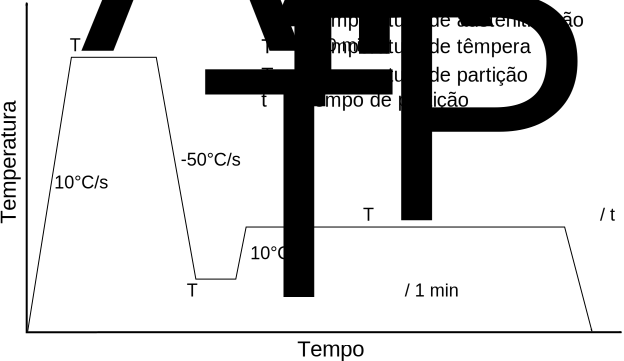
\includegraphics[height=8cm]{img/expproc_dil.pdf}
	\caption{Ilustração esquemática do ciclo térmico de Têmpera e Partição aplicado nas amostras de dilatometria.}
	\label{fig:expDil}
\end{figure}

O experimento para determinação da temperatura Ms consistiu do aquecimento da amostra até a temperatura de austenitização selecionada, seguindo rampa de aquecimento de 10 °C/s, sendo mantida nesta temperatura por 1800 segundos. Em seguida, a amostra foi resfriada até a temperatura de -100 °C sob taxa de resfriamento de --50 °C/s utilizando gás He refrigerado por $N_2$ líquido. O resfriamento até esta temperatura permitiu que a curva da transformação martensítica fosse determinada por completo. Para que o resfriamento até temperaturas abaixo de zero pudesse ser realizado no equipamento, a geometria da amostra utilizada foi de cilindro oco, como representado na figura \ref{fig:CPdil}b.

\subsection{Difra\c{c}\~{a}o de raios X \enfase{in situ}}

Tratamentos térmicos com acompanhamento em tempo real (\enfase{in situ}) da evolução de fases por difração de raios X gerados por fonte de luz síncrotron foram realizados na estação experimental \siglaestrangeira{XTMS}{X-ray Scattering and Thermo-Mechanical Simulation}, operada conjuntamente pelo \sigla{LNNano}{Laboratório Nacional de Nanotecnologia}  e pelo \sigla{LNLS}{Laboratório Nacional de Luz Síncrotron} na cidade de Campinas. A instalação da linha XTMS consiste de um avançado simulador termomecânico especialmente construído para ser usado em experimentos de difração de raios X. O simulador, chamado de Gleeble\textregistered{} 3S50, foi desenvolvido em cooperação da empresa estadunidense \siglaestrangeira{DSI}{Dynamic Systems Inc.} e de corpo técnico-científico do LNNano com o propósito de efetuar testes termomecânicos com controle de temperatura e solicitação mecânica em amostras macroscópicas, enquanto aquisições simultâneas de difração de raios X são obtidas. %A figura xx mostra a configuração da instalação no blablabla

No interior da câmara do simulador Gleeble os corpos de prova são presos por garras de cobre, por meio das quais é conduzida corrente elétrica para aquecimento das amostras por efeito Joule. O controle da potência é feito por algoritmo proporcional integral derivativo (PID), sendo que a resposta de temperatura é obtida por meio de termopares (tipo K, Alumel/Cromel) soldados às amostras.

A instalação conta com um goniômetro de alta resolução montado ao redor do simulador. O goniômetro é montado sobre uma mesa de alinhamento que permite o posicionamento do plano de difração sobre a superfície da amostra. Os detetores para contagem de fótons ficam localizados no goniômetro e podem ser posicionados em ângulos entre 0 e 150° e a uma distância mínima da superfície da amostra de 361 mm. Neste trabalho, foram utilizados dois detetores Mythen 1K, cada um possuindo 1280 canais de aquisição (pixels) de 50 $\mu$m de largura. Na distância mínima de trabalho, cada detetor cobre uma faixa de ângulos de aproximadamente 10°, totalizando um ângulo de cobertura de cerca de 20°.

Para os experimentos, corpos de prova do ferro fundido foram usinados na geometria esquematizada na figura \ref{fig:CPXTMS}. Durante o posicionamento das amostras no interior da câmara do simulador procurou-se estabelecer o ângulo $\omega$ de 15° entre a superfície da amostra e o feixe incidente de raios X. Em sequência, as amostras foram submetidas a ciclos de Têmpera e Partição segundo as condições de tratamento térmico pré-determinadas.

\simbolo{$\omega$}{Ângulo estabelecido entre o feixe de raios X incidente e a superfície da amostra}

Assim como nos ensaios de dilatometria realizados no dilatômetro Bähr, as amostras foram austenitizados durante 30 min, resfriadas até as temperaturas de têmpera e em seguida reaquecidas até as temperaturas de partição, em que foram mantidas durante 1800 segundos. Nas etapas de resfriamento não foi utilizado resfriamento forçado por meio convectivo, de modo que a extração de calor foi feita unicamente por meio das garras de cobre em contato com os corpos de prova. Consequentemente, taxas de resfriamento inferiores às obtidas no dilatômetro Bähr foram conseguidas no simulador Gleeble. Contudo, análise metalográfica posterior mostrou que a taxa de resfriamento utilizada foi suficiente para garantir a transformação martensítica na etapa de têmpera.

\begin{figure}
	\includegraphics[width=14cm]{img/CPXTMS.pdf}
	\caption{Desenho esquemático do corpo de prova utilizado na estação experimental XTMS. Dimensões em  milímetros.}
	\label{fig:CPXTMS}
\end{figure}

Paralelamente à realização dos tratamentos térmicos foram feitas aquisições de difração de raios X. A energia do feixe foi estabelecida em 12 keV, equivalente ao comprimento de onda $\lambda = 1,033\text{\AA}$, utilizando monocromador de Si(111). As fendas de limitação de fluxo de fótons foram ajustadas para permitirem que apenas uma região de 2 x 0,5 mm\textsuperscript{2} do feixe incidisse sobre a superfície da amostra. Durante as aquisições em tempo real, o goniômetro foi fixado no ângulo 2$\theta$ de 31° e os detetores Mythen foram aproximados até a distância mínima de trabalho de 361 mm. Nesta configuração, os detetores cobriram a faixa de ângulos de difração de 26 a 47°, na qual foi possível monitorar a evolução dos picos de difração (110) e (200) da ferrita e (111) e (200) da austenita em tempo real.

\simbolo{2$\theta$}{Ângulo de difração} %definir tth melhor aqui.

Dependendo da etapa do tratamento térmico, foram utilizados diferentes tempos e frequências de aquisição de dados. Durante a etapa isotérmica de partição, cuja análise é enfatizada neste trabalho, aquisições foram feitas usando tempo de exposição de 3 segundos, espaçadas a cada 0,5 segundos. Ao final da etapa de partição e do tratamento térmico foram feitas varreduras do ângulo de difração entre 26 e 86° a 10 segundos de exposição por passo, de modo a obter um número de picos de difração substantivo para quantificação das fases. A figura \ref{fig:esqXTMS} ilustra a programação do experimento na instalação XTMS.

\begin{figure}
	\includegraphics[height=10cm]{img/expproc_XTMS.pdf}
	\caption{Ilustração esquemática do teste programado na instalação XTMS.}
	\label{fig:esqXTMS}
\end{figure}

Antes de cada experimento a câmara do simulador Gleeble foi evacuada por um sistema de vácuo composto de bomba mecânica e difusora. Os níveis de vácuo atingidos foram consistentemente inferiores a $1 \times 10^{-2}$ torr. Um bom nível de vácuo é imprescindível para que a oxidação e a descarbonetação do material em sua superfície sejam evitadas durante o aquecimento e a aquisição dos difratogramas.

\subsubsection{An\'{a}lise dos resultados de DRX}

Uma vez que a amostra fica posicionada em um ângulo $\omega$ fixo em relação ao feixe de raios X, a geometria de difração $\omega$--$2\theta$ utilizada difere fundamentalmente das geometrias convencionais dos métodos de Bragg-Brentano ($\theta$--$2\theta$) e Debye-Scherrer (feixe transmitido). A interpretação dos padrões de difração, no entanto, seguiu procedimentos semelhantes de indexação e determinação dos parâmetros de rede das fases.

A análise dos difratogramas obtidos durante os tratamentos isotérmicos foi feita por meio de rotinas programadas em Rscript. Os picos de difração obtidos foram ajustados segundo a equação de distribuição Gaussiana (equação \ref{eq:Gaussiana}) que representa uma função sino que descreve o formato os picos de difração. O autor é ciente que para esta tarefa costuma ser utilizada uma função do tipo Pseudo-Voigt, que descreve melhor o alargamento instrumental associado aos picos de difração. Todavia, devido ao custo de processamento computacional e problemas no ajuste de picos superpostos utilizando essa função, optou-se pelo uso de perfis Gaussianos, que demonstraram fornecer resultados satisfatórios.

\begin{equation}
	I = I_0 \exp{\left[-\left(\frac{2\theta - 2\theta_0}{w}\right)^2\right]} + bck
	\label{eq:Gaussiana}
\end{equation}

Na equação \ref{eq:Gaussiana}, $I$ corresponde à intensidade de difração observada em função do ângulo $2\theta$, $I_0$ é a intensidade máxima medida no ângulo de difração $2\theta_0$, $w$ é a largura do pico Gaussiano e $bck$ contabiliza o sinal de fundo (\enfase{background}), que tem seu valor assumido como constante. As áreas integradas ($A_{hkl}$) sob os picos foram calculadas pela integração da curva Gaussiana usando a equação \ref{eq:intGauss}, sendo convertidas para frações volumétricas de fases pela equação \ref{eq:fracDRX}, conforme metologia descrita por \citaremsentenca{Cullity2001}.

\begin{align}
	A &= \int\limits_{-\infty}^{\infty} I_0 \exp{\left[-\left(\frac{2\theta - 2\theta_0}{w}\right)^2\right]} d \theta \nonumber \\
	&= I_0 |w| \sqrt{\pi}
	\label{eq:intGauss}
\end{align}

\begin{equation}
	f^\gamma = 1 - f^\alpha = \frac{\sum A_{hkl}^\gamma/R_{hkl}^\gamma}{\sum A_{hkl}^\alpha/R_{hkl}^\alpha + \sum A_{hkl}^\gamma/R_{hkl}^\gamma}
	\label{eq:fracDRX}
\end{equation}

A equação \ref{eq:fracDRX} faz uso dos coeficientes $R_{hkl}$ que contabilizam o efeito dos fatores que compõem o cálculo da intensidade teórica dos picos de difração. Na tabela \ref{tab:fatoresR} são apresentados os valores de $R_{hkl}$ utilizados para quantificação das fases neste trabalho.

\begin{table} %REVISAR ANTES DE IMPRIMIR!
	\caption{Coeficientes $R_{hkl}$ calculados para as fases ferrita ($\alpha$) e austenita ($\gamma$) do ferro puro\cite{Cullity2001}.}
	\begin{tabular}{c c c ' c c c}
	\thickhline
	Fase & hkl & $R_{hkl}$ & Fase & hkl & $R_{hkl}$\\
	\hline
	& 110 & 1840 & & 111 & 1351\\
	& 200 & 288,6 & & 200 & 644,3\\
	$\alpha$ & 211 & 530,0 & $\gamma$ & 220 & 376,7\\
	& 220 & 142,5 & & 311 & 390\\
	& 310 & 172,8 & & 222 & 107,9\\
	\thickhline
	\end{tabular}
	\label{tab:fatoresR}
\end{table}

A variação do parâmetro de rede da austenita ao longo do tratamento isotérmico também foi avaliada pelos resultados de DRX. A partir do cálculo do espaçamento interplanar $d_{hkl}$ pela lei de Bragg (equação \ref{eq:Bragg}), o parâmetro de rede da austenita $a^\gamma$ foi determinado pela equação \ref{eq:parametroRede}, que, para sistemas cristalinos cúbicos, estabelece a relação entre o parâmetro de rede da fase e a distância interplanar entre planos de índices de Miller $hkl$.

\begin{equation}
	n\lambda = 2d_{hkl}\,sen(\theta_0)
	\label{eq:Bragg}
\end{equation}

\begin{equation}
	d_{hkl}^\gamma = \frac{a^\gamma}{\sqrt{h^2 + k^2 + l^2}}
	\label{eq:parametroRede}
\end{equation}

A variação do parâmetro de rede foi interpretada pelo enriquecimento em carbono da austenita durante a etapa de partição do tratamento T\&P. Dessa forma, a variação do teor de carbono foi estimada por meio da equação empírica obtida por \citaremsentenca{Dyson1970}, que leva em conta a variação do parâmetro de rede da austenita em função de sua composição química:

\begin{equation}
	a^\gamma = 3,5780 + 3,30\cdot10^{-2} \%w_C^\gamma + 9,5\cdot10^{-4} \%w_{Mn}^\gamma + 1,5\cdot10^{-3} \%w_{Cu}^\gamma
	\label{eq:DysonHolmes}
\end{equation}
%
em que $\%w_i^\gamma$ é a porcentagem em massa do elemento $i$ (= C, Mn, Cu) dissolvido na austenita. A equação original também descreve a contribuição de outros elementos no parâmetro de rede da austenita. No entanto, suas representações na equação acima foram poupadas, devido a seus baixos teores na liga estudada. Dyson e Holmes argumentam que o silício, que aparece em quantidade substancial no ferro fundido, apresenta efeito desprezível na distorção do reticulado da austenita e, por esse motivo, sua contribuição não foi incorporada à equação.

Uma vez que as aquisições foram feitas a temperaturas elevadas, para que os valores de $a^\gamma$ obtidos pelos difratogramas pudessem ser interpretados na temperatura ambiente pelo método descrito acima, previamente à aplicação da equação \ref{eq:DysonHolmes}, o efeito da expansão térmica no parâmetro de rede da austenita foi corrigido utilizando a equação desenvolvida por \citaremsentenca{VanBohemen2013b}:

\begin{equation}
	\frac{\Delta L^\gamma}{L_0^\gamma} = B_\gamma T + B_\gamma \Theta_D^\gamma \left[ \exp{\left( -\frac{T}{\Theta_D^\gamma} \right)}\right]
	\label{eq:expTermica}
\end{equation}

A equação \ref{eq:expTermica} descreve a variação de comprimento $\Delta L^\gamma$ de uma amostra completamente austenítica na temperatura absoluta $T$ em relação a seu comprimento $L_0^\gamma$ extrapolado para o estado de referência a 0 K. $B^\gamma$ e $\Theta_D^\gamma$ são constantes de ajuste determinadas pela regressão linear de dados disponíveis na literatura e valem $B^\gamma = 24,8 \times 10^{-6} K^{-1}$ e $\Theta_D^\gamma = 280 K$.

\subsection{Caracteriza\c{c}\~{a}o microestrutural}

Para análise da microestrutura das amostras, estas foram submetidas a preparação metalográfica, que consistiu do embutimento das amostras em baquelite, lixamento em lixa d'água até granulometria 1200 e subsequente polimento em pastas de diamante de 6, 3 e 1 $\mu$m. Por fim, as amostras foram submetidas a ataques metalográficos com reagentes químicos adequados para cada propósito. Para observação no microscópio óptico, as amostras foram pré-atacadas com o reagente Nital 2\% ($etanol + 2\%vol\,HNO_3$), sendo logo em seguida lavadas sob água corrente com detergente neutro e algodão, e subsequentemente imersas em solução do reagente Beraha ($3g\,K_2S_2O_5 + 10g\,Na_2S_2O_3 + 100mL\,H_2O$) por 60 segundos. O reagente Beraha, assim como outros reagentes que produzem ataques seletivos em ligas ferrosas, colore a ferrita, deixando-a marrom quando observada no microscópio óptico. De forma semelhante acontece com a martensita, que se apresenta tingida sob ação deste reagente. Por sua vez, a austenita fica isenta do ataque e, consequentemente, aparece branca nas micrografias\cite{MetalsVol9}. Para observação no \sigla{MEV}{Microscópio Eletrônico de Varredura}, as amostras foram apenas atacadas utilizando o reagente Nital 2\%.

Para obtenção de imagens de microscopia óptica foi utilizado um microscópio óptico Olympus BX60M com câmera CCD acoplada, localizado nas dependências do \sigla{LCMHC}{Laboratório de Caracterização Microestrutural Hubertus Colpaert} do \sigla{PMT-USP}{Departamento de Engenharia Metalúrgica e de Materiais da EPUSP}. As imagens de microscopia eletrônica de varredura foram obtidas tanto no microscópio de feixe de emissão de campo (MEV-FEG) FEI Inspect F50 com sistemas de \sigla{EDS}{Análise de Energia Dispersiva} e \sigla{EBSD}{Difração de Elétrons Retroespalhados} acoplados a ele. Estes equipamentos estão situados no \sigla{LabMicro}{Laboratório de Microscropia Eletrônica e de Força Atômica}, também vinculado ao PMT-USP.

\novasigla{MEV-FEG}{Microscópio Eletrônico de Varredura de Feixe de Emissão de Campo}

\chapter{Resultados parciais e Discuss\~{a}o}

Salvo menção contrária, os valores em porcentagem expressos neste capítulo se referem à base de cálculo em função da massa.

\section{Experimentos preliminares}

Nas figuras \ref{fig:thermocalc}a e \ref{fig:thermocalc}b são mostrados o mapa de predominância de fases para a liga estudada e a variação da concentração de carbono dissolvido nas fases em equilíbrio. Ambas as figuras foram construídas por meio de simulações no software Thermo-Calc\textregistered{} utilizando o banco de dados TCFE. Para simplificação do problema, foram consideradas no cálculo apenas os principais elementos presentes na elaboração da liga, isto é, Fe, C, Si, Mn e Cu.

É possível perceber que a grafita é presente em uma ampla faixa de temperaturas no ferro fundido. Isso se dá devido à composição da liga, próxima à do eutético. Por este motivo, durante a austenitização do material, necessariamente a grafita coexistirá em equilíbrio com a austenita. Neste trabalho, a terminologia ``austenitização plena'' é utilizada para descrever a etapa de austenitização neste campo de duas fases, sendo que os cálculos termodinâmicos apontam que essa condição é obtida em temperaturas superiores a 814 °C. Em temperaturas intermediárias a 814 °C e 782 °C é prevista a existência de um campo de três fases, denominado ``campo intercrítico'', no qual é estabelecido o equilíbrio termodinâmico as fases ferrita, austenita e grafita.

\begin{figure}
	\subfloat[]{\includegraphics[width=7.5cm]{img/thermo-calc/NPvsT.png}}
	\quad
	\subfloat[]{\includegraphics[width=7.5cm]{img/thermo-calc/CvsT.png}}
	\caption{Comportamento das frações de fases (a) e teor de carbono dissolvido nas fases em equilíbrio (b) em função da temperatura.}
	\label{fig:thermocalc}
\end{figure}

Os resultados obtidos no Thermo-Calc\textregistered{} também mostram como varia o teor de carbono dissolvido na austenita em função da temperatura. Nota-se que temperaturas maiores implicam em uma maior solubilidade do carbono na austenita, como já fora apontado na seção \ref{subsec:ADI}. A 814 °C, por exemplo, prevê-se que a austenita possuirá 0,59\%, enquanto que a 900 °C a solubilidade do carbono na austenita deverá ser de 0,81\%. Dessa forma, a martensita formada durante a têmpera após a austenitização em temperaturas mais elevadas tende a possuir morfologia de placas grossas e frágeis, enquanto temperaturas mais baixas devem gerar uma mistura de martensita em ripas e martensita em placas.

Para aferir as temperaturas correspondentes aos campos intercrítico e de austenitização plena previstas pelo Thermo-Calc\textregistered{} foi realizado um experimento de dilatometria para determinar as temperaturas críticas de transformação do material. Nas figuras \ref{fig:dilTempera}a e \ref{fig:dilTempera}b é mostrada a curva de dilatação para o ciclo de aquecimento do material e o resfriamento final. Em temperaturas inferiores a 737 °C (região A na figura \ref{fig:dilTempera}b) o material se dilata de forma aproximadamente linear, condizente com a expansão material em função do aumento da agitação térmica. A 737 °C, no entanto, é observada um súbito aumento da velocidade de expansão, observada em detalhe na figura \ref{fig:dilTempera}b, tendência que persiste até a temperatura de 783 °C (região B). Esta expansão é interpretada como a dissolução de carbonetos da microestrutura como recebida e formação de grafita, fase estável nesta temperatura. Entre 783 °C e 854 °C (região C) o material sofre outra transformação de fase, que leva a contração do material. Esta transformação, por sua vez, é associada à formação da fase compacta austenita, mais densa que os demais constituintes do ferro fundido. A partir de 854 °C (região D) a dilatação do material volta a ser aproximadamente linear, compatível com a expansão térmica da mistura de austenita e grafita.

\begin{figure}
	\subfloat[]{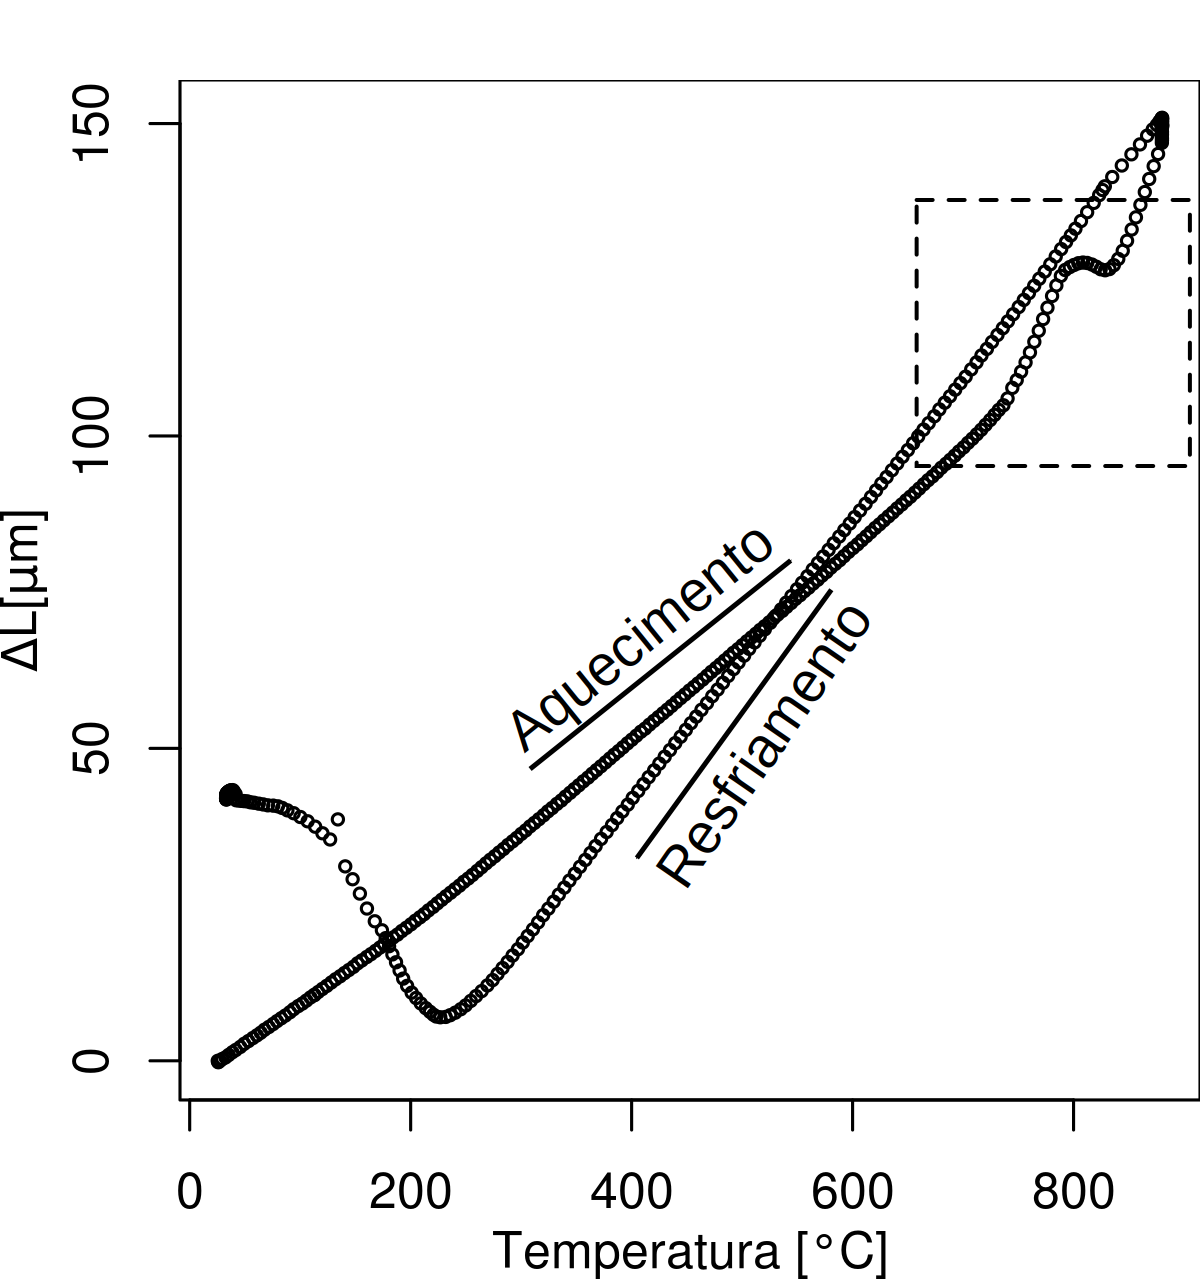
\includegraphics[height=7cm]{img/dilatometria/1_fofoTupy_10oCmin_2.png}}
	\quad
	\subfloat[]{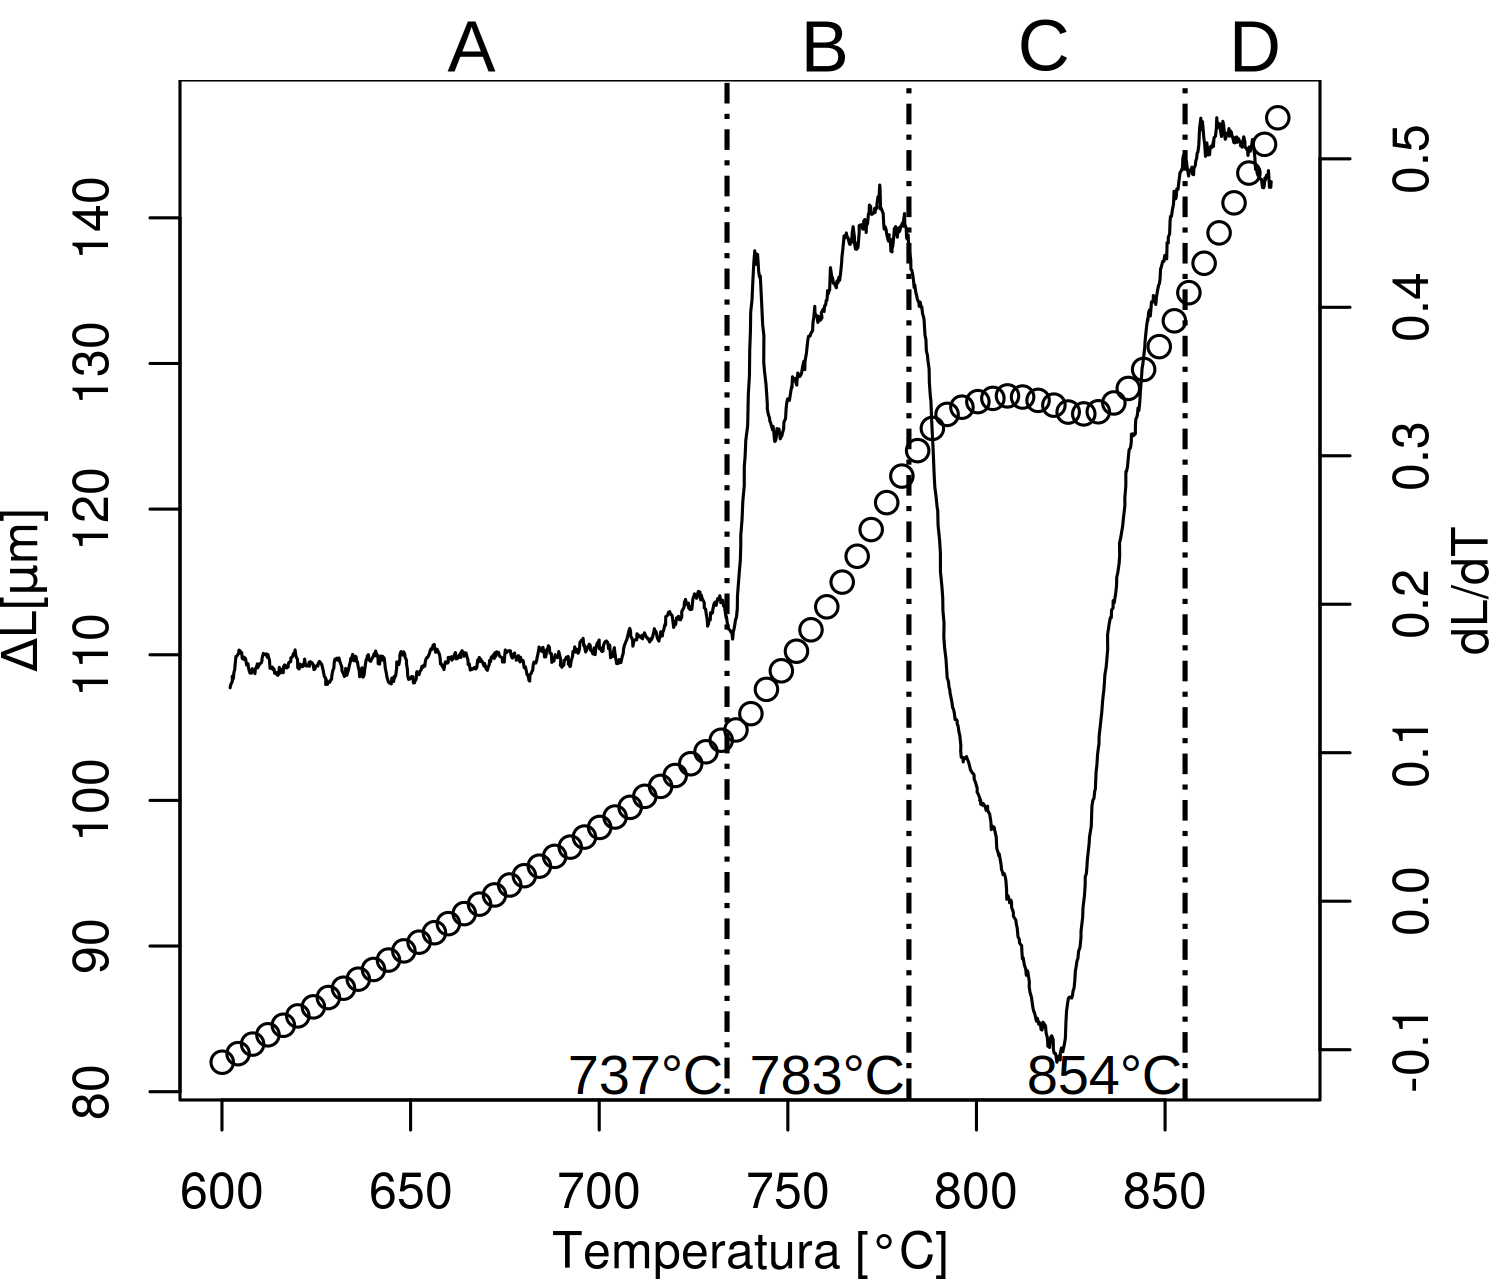
\includegraphics[height=7cm]{img/dilatometria/1_fofoTupy_10oCmin.png}}
	\caption{Curva de dilatação ($\Delta L$) em função da temperatura para o ferro fundido aquecido a 10 °C/min até a temperatura de 880 °C. (a) Curva completa. (b) Detalhe da curva (a) indicado pelo retângulo tracejado. A linha sólida corresponde à derivada numérica ($dL/dT$) da curva de dilatação em função da temperatura.}
	\label{fig:dilTempera}
\end{figure}

Quando comparada com os resultados da simulação termodinâmica, a interpretação da curva de dilatação mostra uma relação coerente entre a temperatura inferior do campo intecrítico (782 °C pelo Thermo-Calc\textregistered{} e 783 °C pela dilatometria), mas mostra uma discrepância entre as temperaturas de austenitização plena obtidas pelos dois métodos (814 °C pelo Thermo-Calc\textregistered{} e 854 °C pela dilatometria). Essa diferença pode ser justificada pela microsegregação do ferro fundido, que produz regiões com menor concentração de elementos gamagênicos, elevando localmente a temperatura de austenitização plena. Outra possibilidade é a própria inabilidade do banco de dados TCFE prever acuradamente o equilíbrio termodinâmico em sistemas complexos, uma vez que o software realiza extrapolações de informações termodinâmicas para prever os potenciais químicos dos elementos.

Para escolha da temperatura de austenitização, tomou-se como referência a menor temperatura em que se dá a austenitização plena do material, isto é, 854 °C. Uma menor temperatura de austenitização leva a uma austenita com menos carbono, implicando em uma martensita de caráter menos frágil do que a obtida em temperaturas mais elevadas de austenitização. Por outro lado, temperaturas elevadas beneficiam a homogeneização da segregação presente no material. Dessa forma, procurou-se adotar uma temperatura intermediária, que gerasse uma martensita de aspecto menos frágil, ao mesmo tempo que parte da heterogeneidade decorrente da segregação pudesse ser eliminada.

Dado o exposto, foi escolhida a temperatura de austenitização de 880 °C para os experimentos subsequentes. Nesta temperatura, o cálculo termodinâmico no software Thermo-Calc\textregistered{} prevê a composição química na austenita segundo a tabela \ref{tab:CQaust}.

\begin{table}
	\caption{Composição química da austenita determinada por cálculo termodinâmico no software Thermo-Calc\textregistered{}.}
	\begin{tabular}{c c c c c}
	\thickhline
	\textbf{Elemento} & C & Si & Mn & Cu\\
	\hline
	\textbf{Composição (\% em massa)} & 0,76 & 2.54 & 0,21 & 0,39\\
	\thickhline
	\end{tabular}
	\label{tab:CQaust}
\end{table}

\section{Dilatometria}

\subsection{Determina\c{c}\~{a}o da temperatura Ms}

A figura \ref{fig:dilMartensita}a mostra a curva de dilatação completa do ensaio de dilatometria para determinação da temperatura Ms. A expansão observada durante o resfriamento em torno de 230 °C corresponde à temperatura de início da transformação martensítica (Ms). Essa conclusão somente é possível de ser tomada caso a taxa de resfriamento de --50 °C/s aplicada à amostra tenha sido suficiente para garantir que a decomposição difusional da austenita tenha sido evitada. Análise metalográfica posterior (seção \ref{sec:micros}) confirma essa observação.

\begin{figure}
	\subfloat[]{\includegraphics[height=9cm]{img/dilatometria/dil_martensita.png}}
	\vspace{0pt}
	\subfloat[]{\includegraphics[height=9cm]{img/dilatometria/dil_martensita_close.png}}
	\caption{Curva de dilatação obtida durante o ciclo de austenitização e têmpera. (a) Curva completa. (b) Detalhe da expansão linear decorrente da transformação martensítica.}
	\label{fig:dilMartensita}
\end{figure}

Na figura \ref{fig:dilMartensita}b a expansão associada à reação martensítica é mostrada em detalhe. Em temperaturas superiores à Ms, a matriz do material é completamente austenítica. A dilatação da amostra nestas temperaturas é aproximadamente linear e é atribuída à agitação térmica. Em temperaturas inferiores à Ms a formação da martensita é acompanhada de uma forte expansão que cessa em uma temperatura de término da transformação martensítica (Mf) em que toda a austenita é consumida; nesse caso, a temperatura Mf se encontra em torno de --50 °C.

A fração transformada de martensita a partir da austenita $f^{\alpha\text{\textquoteright}}$ foi calculada utilizando a regra das alavancas, expressa pela equação \ref{eq:levelRule} expressa a seguir:

\begin{equation}
	f^{\alpha\text{\textquoteright}} = 1 - f^\gamma = \frac{A}{A + B}
	\label{eq:levelRule}
\end{equation}
%
em que $f^\gamma$ é a fração não transformada de austenita.

A determinação das variáveis ``A'' e ``B'' são mostradas na construção da figura \ref{fig:dilMartensita}b. ``A'' consiste da expansão associada à transformação martensítica em relação ao comprimento do corpo de prova caso ele permanecesse austenítico na temperatura de têmpera $TT$. Esse comprimento é determinado pela extrapolação do trecho de expansão térmica linear da austenita para a temperatura $TT$. $A + B$ é a expansão teórica do corpo de prova caso a amostra se transformasse completamente em martensita na temperatura $TT$.

A fração não transformada de austenita em função da temperatura de têmpera calculada pelo método exposto é mostrada na figura \ref{fig:KMFoFo}. Os dados experimentais, representados pelos círculos abertos, foram ajustados pelo método dos mínimos quadrados pelo modelo proposto por Koistinen e Marburger (equação \ref{eq:KM}). Na equação obtida o parâmetro de ajuste $\beta$ e a temperatura Ms foram determinados em $-1,23 \times 10^{-2} \text{°C}^{-1}$ e 221,1 °C, respectivamente. Nota-se que a temperatura Ms determinada como parâmetro de ajuste da equação de Koistinen-Marbuger é ligeiramente inferior àquela que corresponde ao início da expansão do corpo de prova em função da formação de martensita. Isso se deve a uma inércia para desencadeamento dos \textit{bursts} de martensita na austenita. Também se percebe que o coeficiente $\beta$ se mostrou bastante próximo ao valor de $-1,1 \times 10^{-2} \text{°C}^{-1}$ obtido no trabalho original de Koistinen e Marburger\cite{Koistinen1959}.

\begin{figure}
	\includegraphics[height=12cm]{img/dilatometria/frac_martensita.png}
	\caption{Fração não transformada de austenita ($f^\gamma$) em função da temperatura de têmpera determinada pelos dados do experimento de dilatometria.}
	\label{fig:KMFoFo}
\end{figure}

Adicionalmente, a equação de Koistinen-Marburger não se ajusta bem aos valores experimentais para baixas temperaturas. Isso pode ser explicado pelo desvio da linearidade da expansão térmica para temperaturas muito baixas, tanto para a martensita, quanto para a austenita, como pontuado por \citaremsentenca{VanBohemen2013b}. A equação, no entanto, é perfeitamente válida para as temperaturas de têmpera utilizadas neste trabalho. Pela equação obtida, prevê-se que cerca de 9\% (em volume) de austenita é retida quando o material é temperado diretamente à temperatura ambiente (25 °C). A tabela \ref{tab:austRetida} mostra as quantidades de austenita não transformada que devem ser obtidas após a etapa de têmpera do ciclo T\&P programadas nos experimentos deste trabalho.

\begin{table}
	\caption{Porcentagem (em volume) de austenita não transformada obtida para diferentes temperaturas de têmpera.}
	\begin{tabular}{c c}
	\thickhline
	Temperatura de têmpera (TT) [°C] & \% em volume de austenita\\
	\hline
	25 &  9,0\\
	140 & 36,9\\ 
	170 & 53,3\\
	200 & 77,1\\
	\thickhline
	\end{tabular}
	\label{tab:austRetida}
\end{table}

\subsection{Resposta dilatom\'{e}trica durante ciclos t\'{e}rmicos T\&P}

As curvas representativas da dilatação e temperatura de um experimento de T\&P são mostradas na figura \ref{fig:TP170-300}a. Nesta condição, após a austenitização a 880 °C a amostra de dilatometria foi resfriada até a temperatura de 170 °C, na qual foi mantida por 60 segundos, sendo em seguida reaquecida até 300 °C e mantida por 15 minutos durante a etapa de partição. O final da etapa de resfriamento da têmpera é mostrado em detalhe na figura \ref{fig:TP170-300}b. Percebe-se que imediatamente após o início da etapa de têmpera a amostra sofre uma significativa expansão volumétrica, decorrente da transformação martensítica. Paralelamente, ocorre uma rápida elevação da temperatura, seguida de sua gradativa diminuição até o estabelecimento da temperatura de têmpera programada (i.e., 170 °C). Essa observação foi feita em todas as amostras submetidas ao ciclo T\&P. Isto acontece porque, devido ao resfriamento rápido, há a formação de um gradiente térmico na amostra que provoca uma diferença entre as temperaturas do núcleo e da superfície. Quando o fluxo de gás He --- utilizando no resfriamento forçado --- para, a temperatura da amostra tende a se homogeneizar, de modo que a superfície é reaquecida com o calor proveniente do centro, acarretando no aumento da temperatura medida pelo termopar. Além disso, a reação martensítica libera um calor latente de transformação, também colaborando para a elevação da temperatura.

\begin{figure}
	\subfloat[]{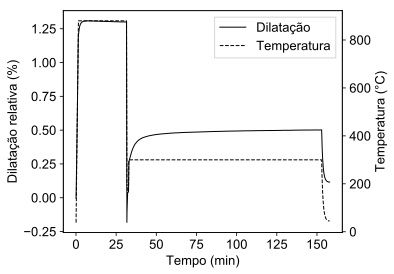
\includegraphics[height=9cm]{img/dilatometria/170-300.png}}
	\vspace{0pt}
	\subfloat[]{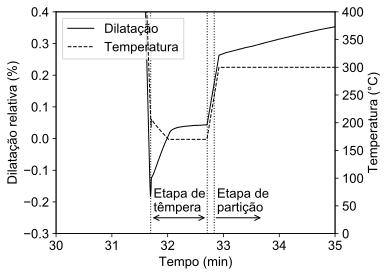
\includegraphics[height=9cm]{img/dilatometria/170-300_close.png}}
	\caption{Curvas de dilatação e temperatura em função do tempo para a amostra temperada a 170 °C e particionada a 300 °C por 15 minutos. (a) Curvas completas. (b) Detalhe do trecho final do resfriamento e do início da etapa de partição.}
	\label{fig:TP170-300}
\end{figure}

As figuras \ref{fig:PT200} a \ref{fig:PT450} mostram as curvas de dilatação durante a etapa isotérmica de partição em função do tempo (figuras com índice ``a'') e as curvas de dilatação em função da temperatura nas etapas adjacentes à etapa de partição (figuras com índice ``b''). Cada figura foi agrupada de acordo com uma temperatura de partição.

\begin{figure}
	\subfloat[]{\includegraphics[width=7.5cm]{img/dilatometria/dilxtime_PT200.png}}
	\quad
	\subfloat[]{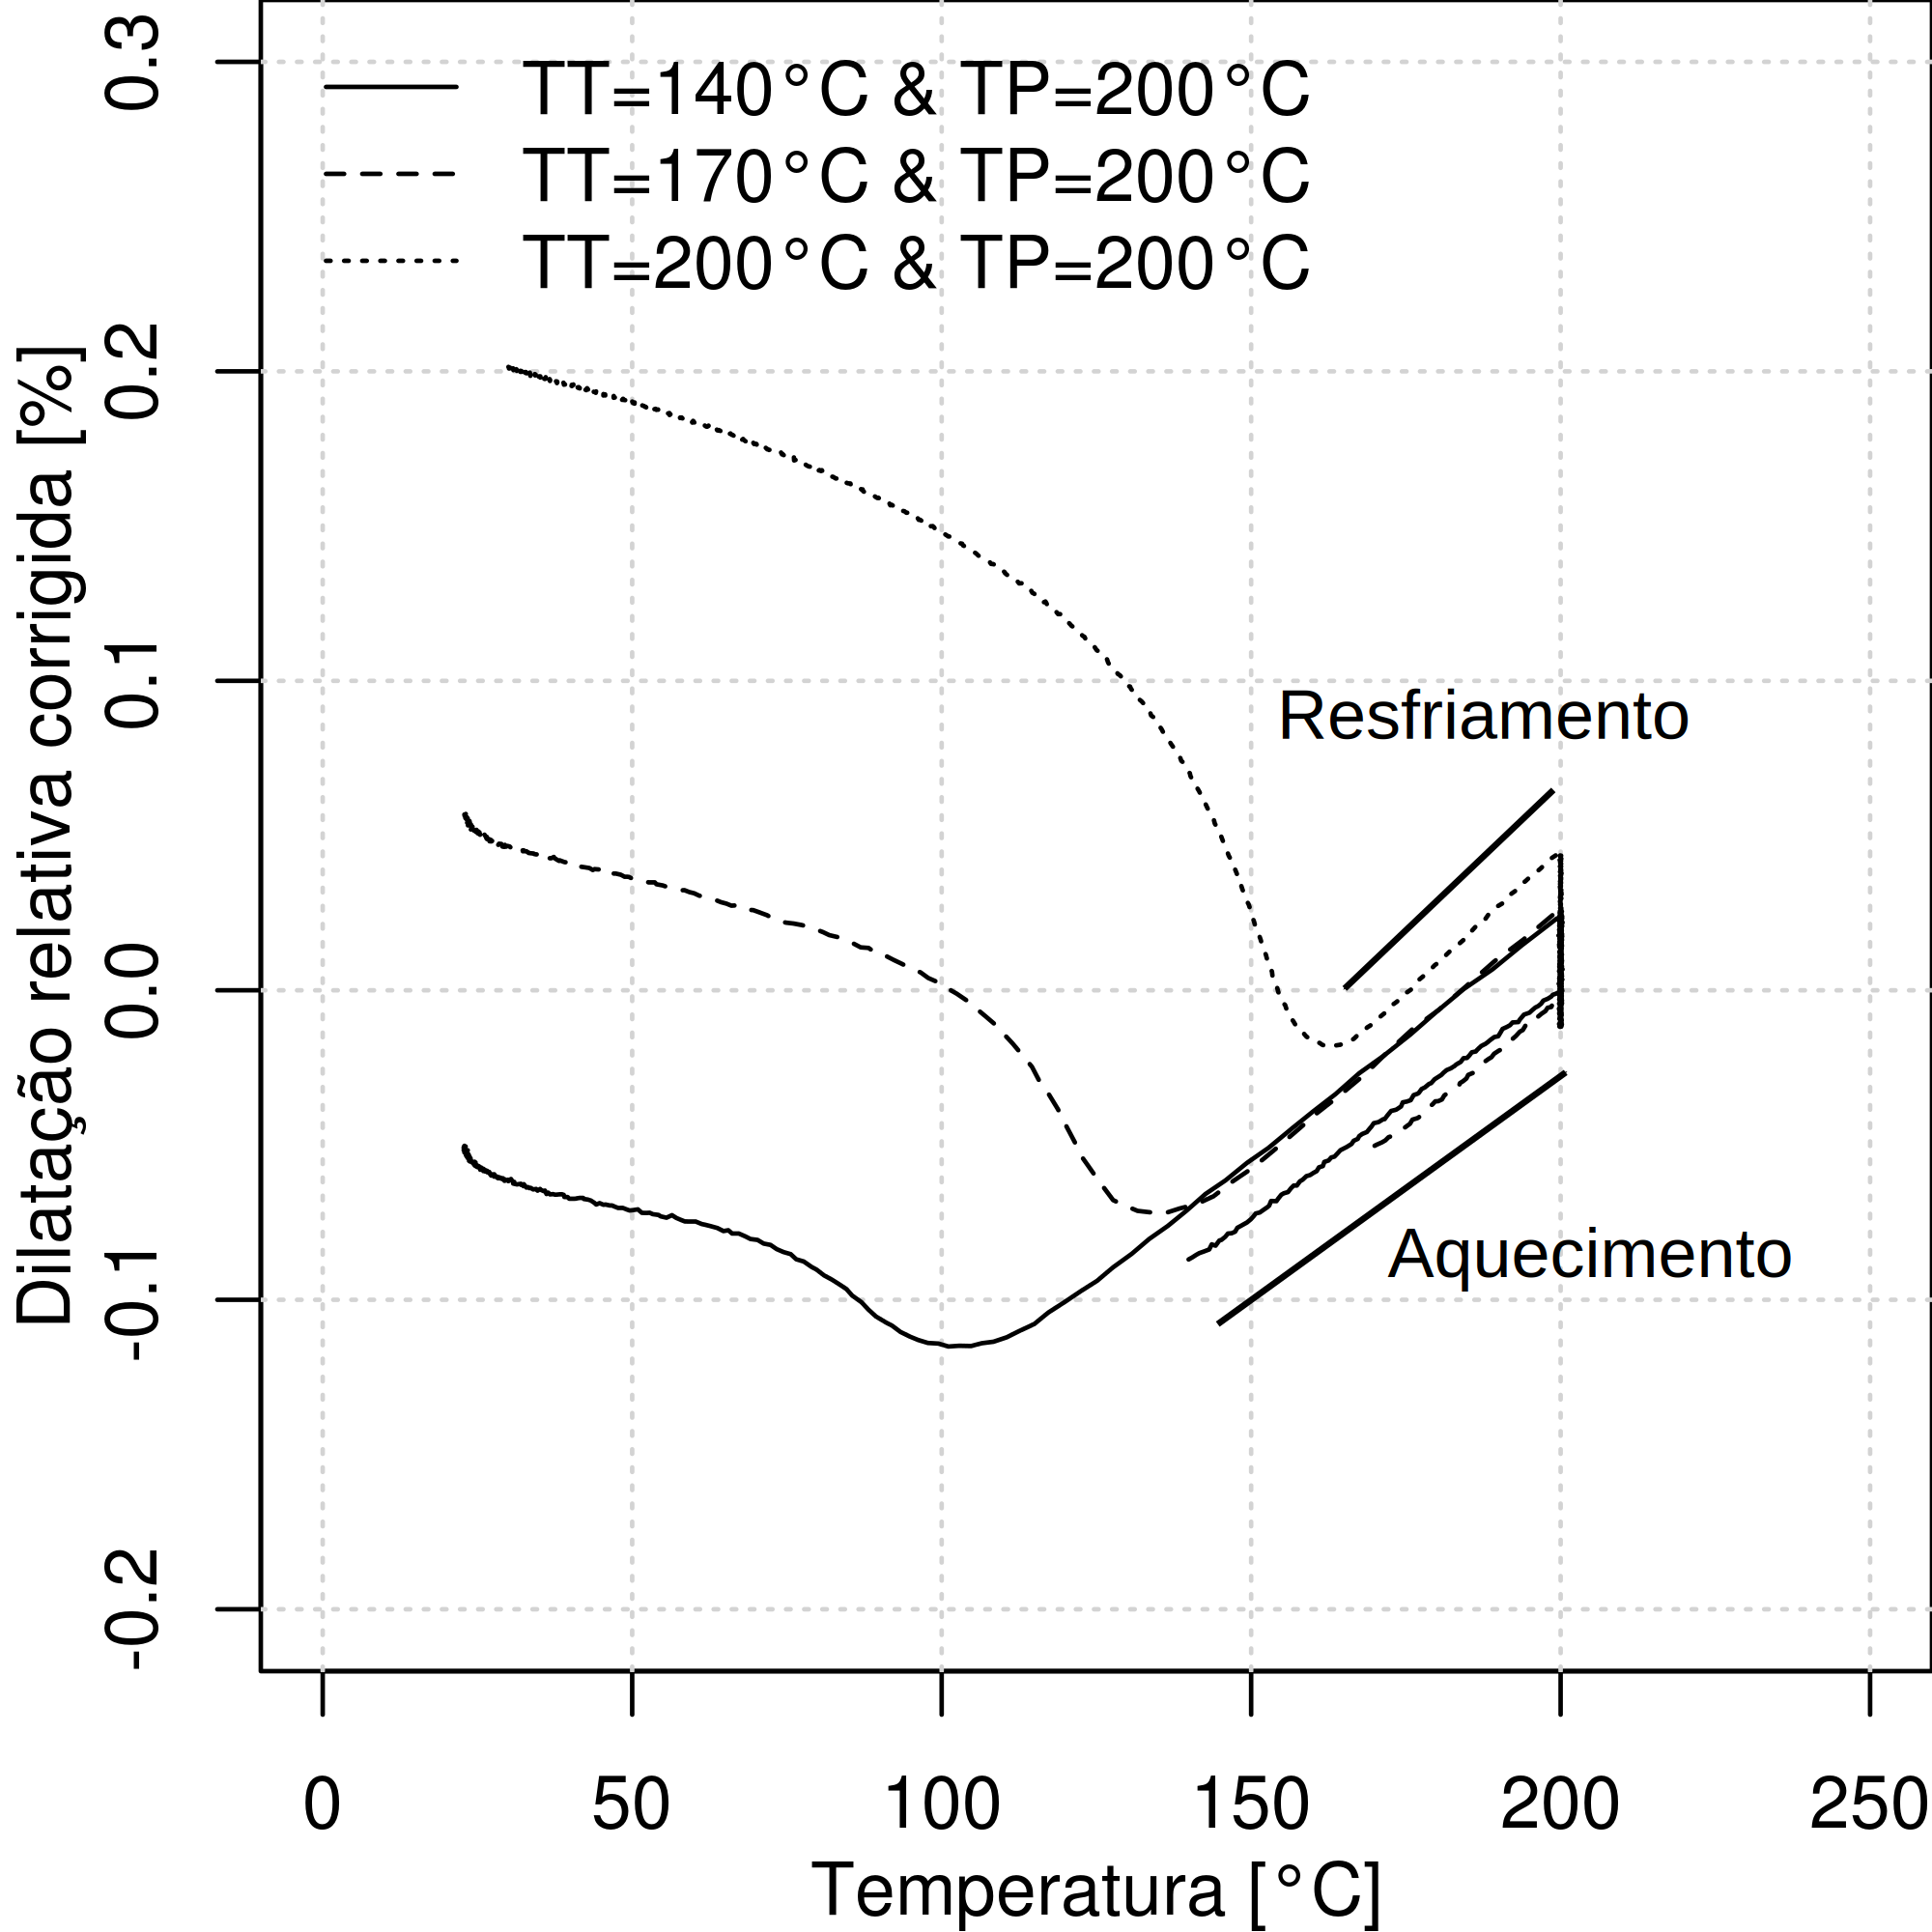
\includegraphics[width=7.5cm]{img/dilatometria/dilxT_PT200.png}}
	\caption{Curvas de dilatação das amostradas particionadas a 200 °C. (a) Dilatação relativa durante a etapa de partição em função do tempo. (b) Dilatação relativa em função da temperatura.}
	\label{fig:PT200}
\end{figure}

\begin{figure}
	\subfloat[]{\includegraphics[width=7.5cm]{img/dilatometria/dilxtime_PT250.png}}
	\quad
	\subfloat[]{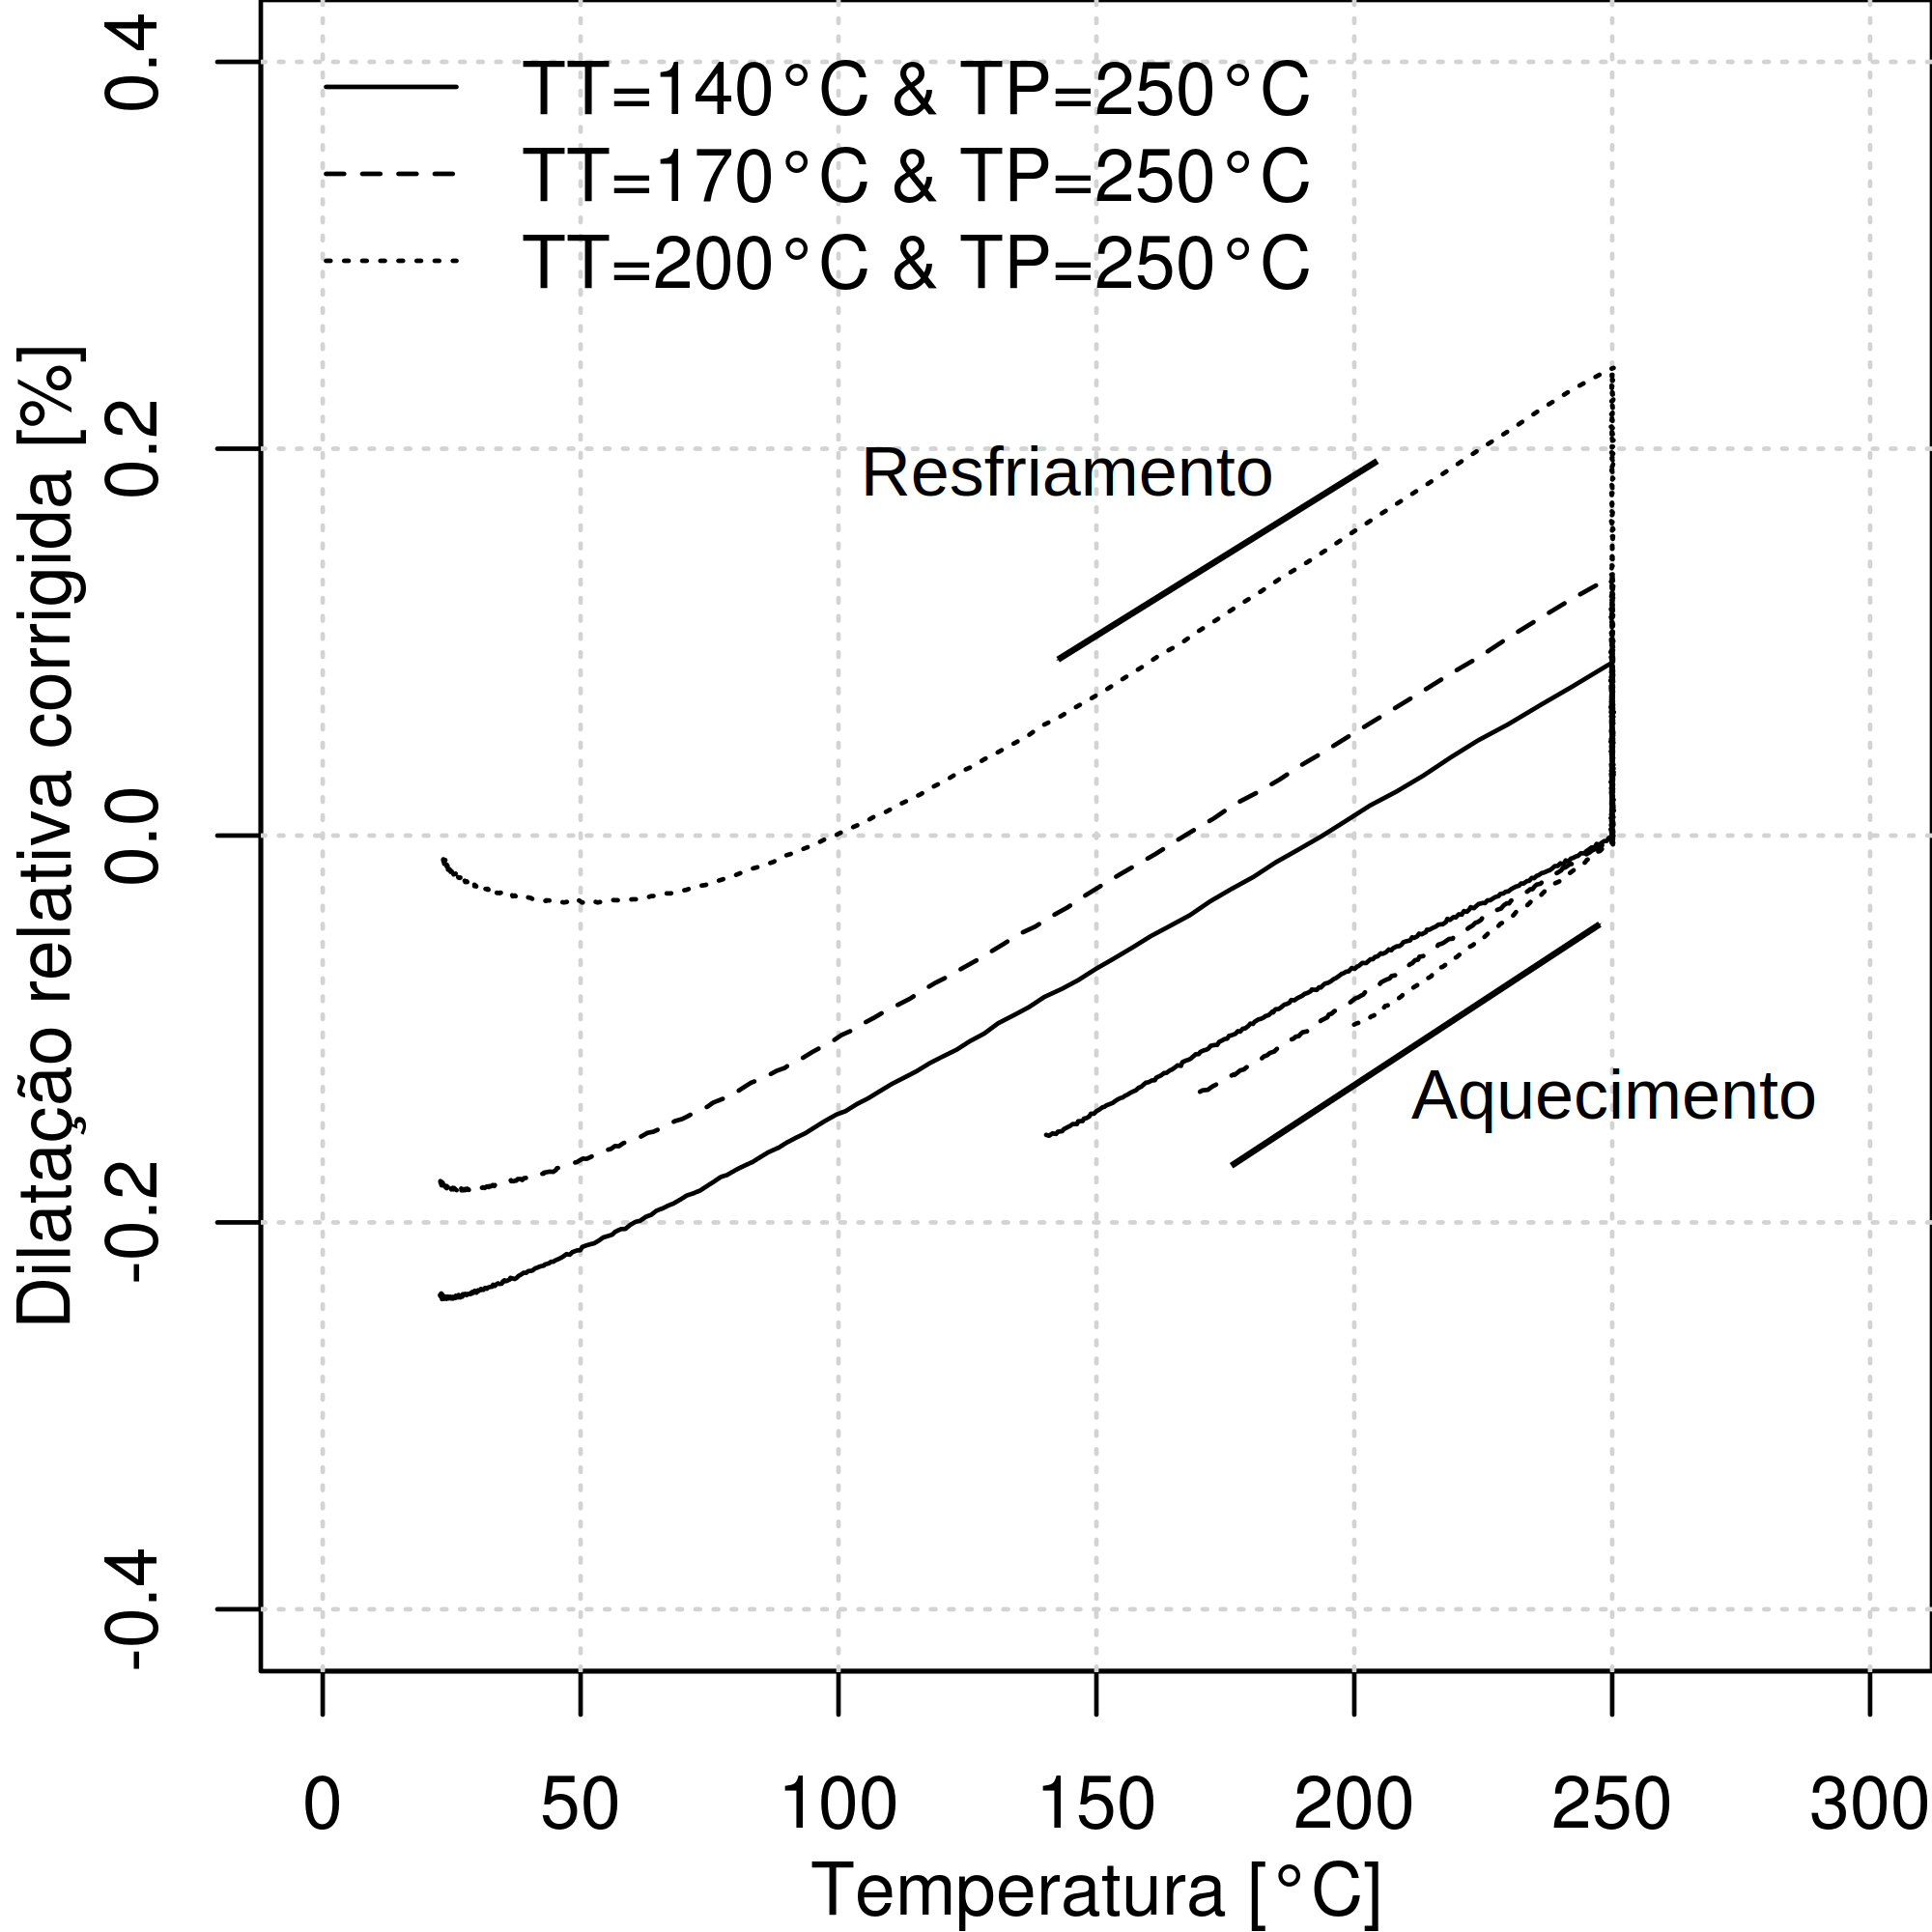
\includegraphics[width=7.5cm]{img/dilatometria/dilxT_PT250.png}}
	\caption{Curvas de dilatação das amostradas particionadas a 250 °C. (a) Dilatação relativa durante a etapa de partição em função do tempo. (b) Dilatação relativa em função da temperatura.}
	\label{fig:PT250}
\end{figure}

\begin{figure}
	\subfloat[]{\includegraphics[width=7.5cm]{img/dilatometria/dilxtime_PT300.png}}
	\quad
	\subfloat[]{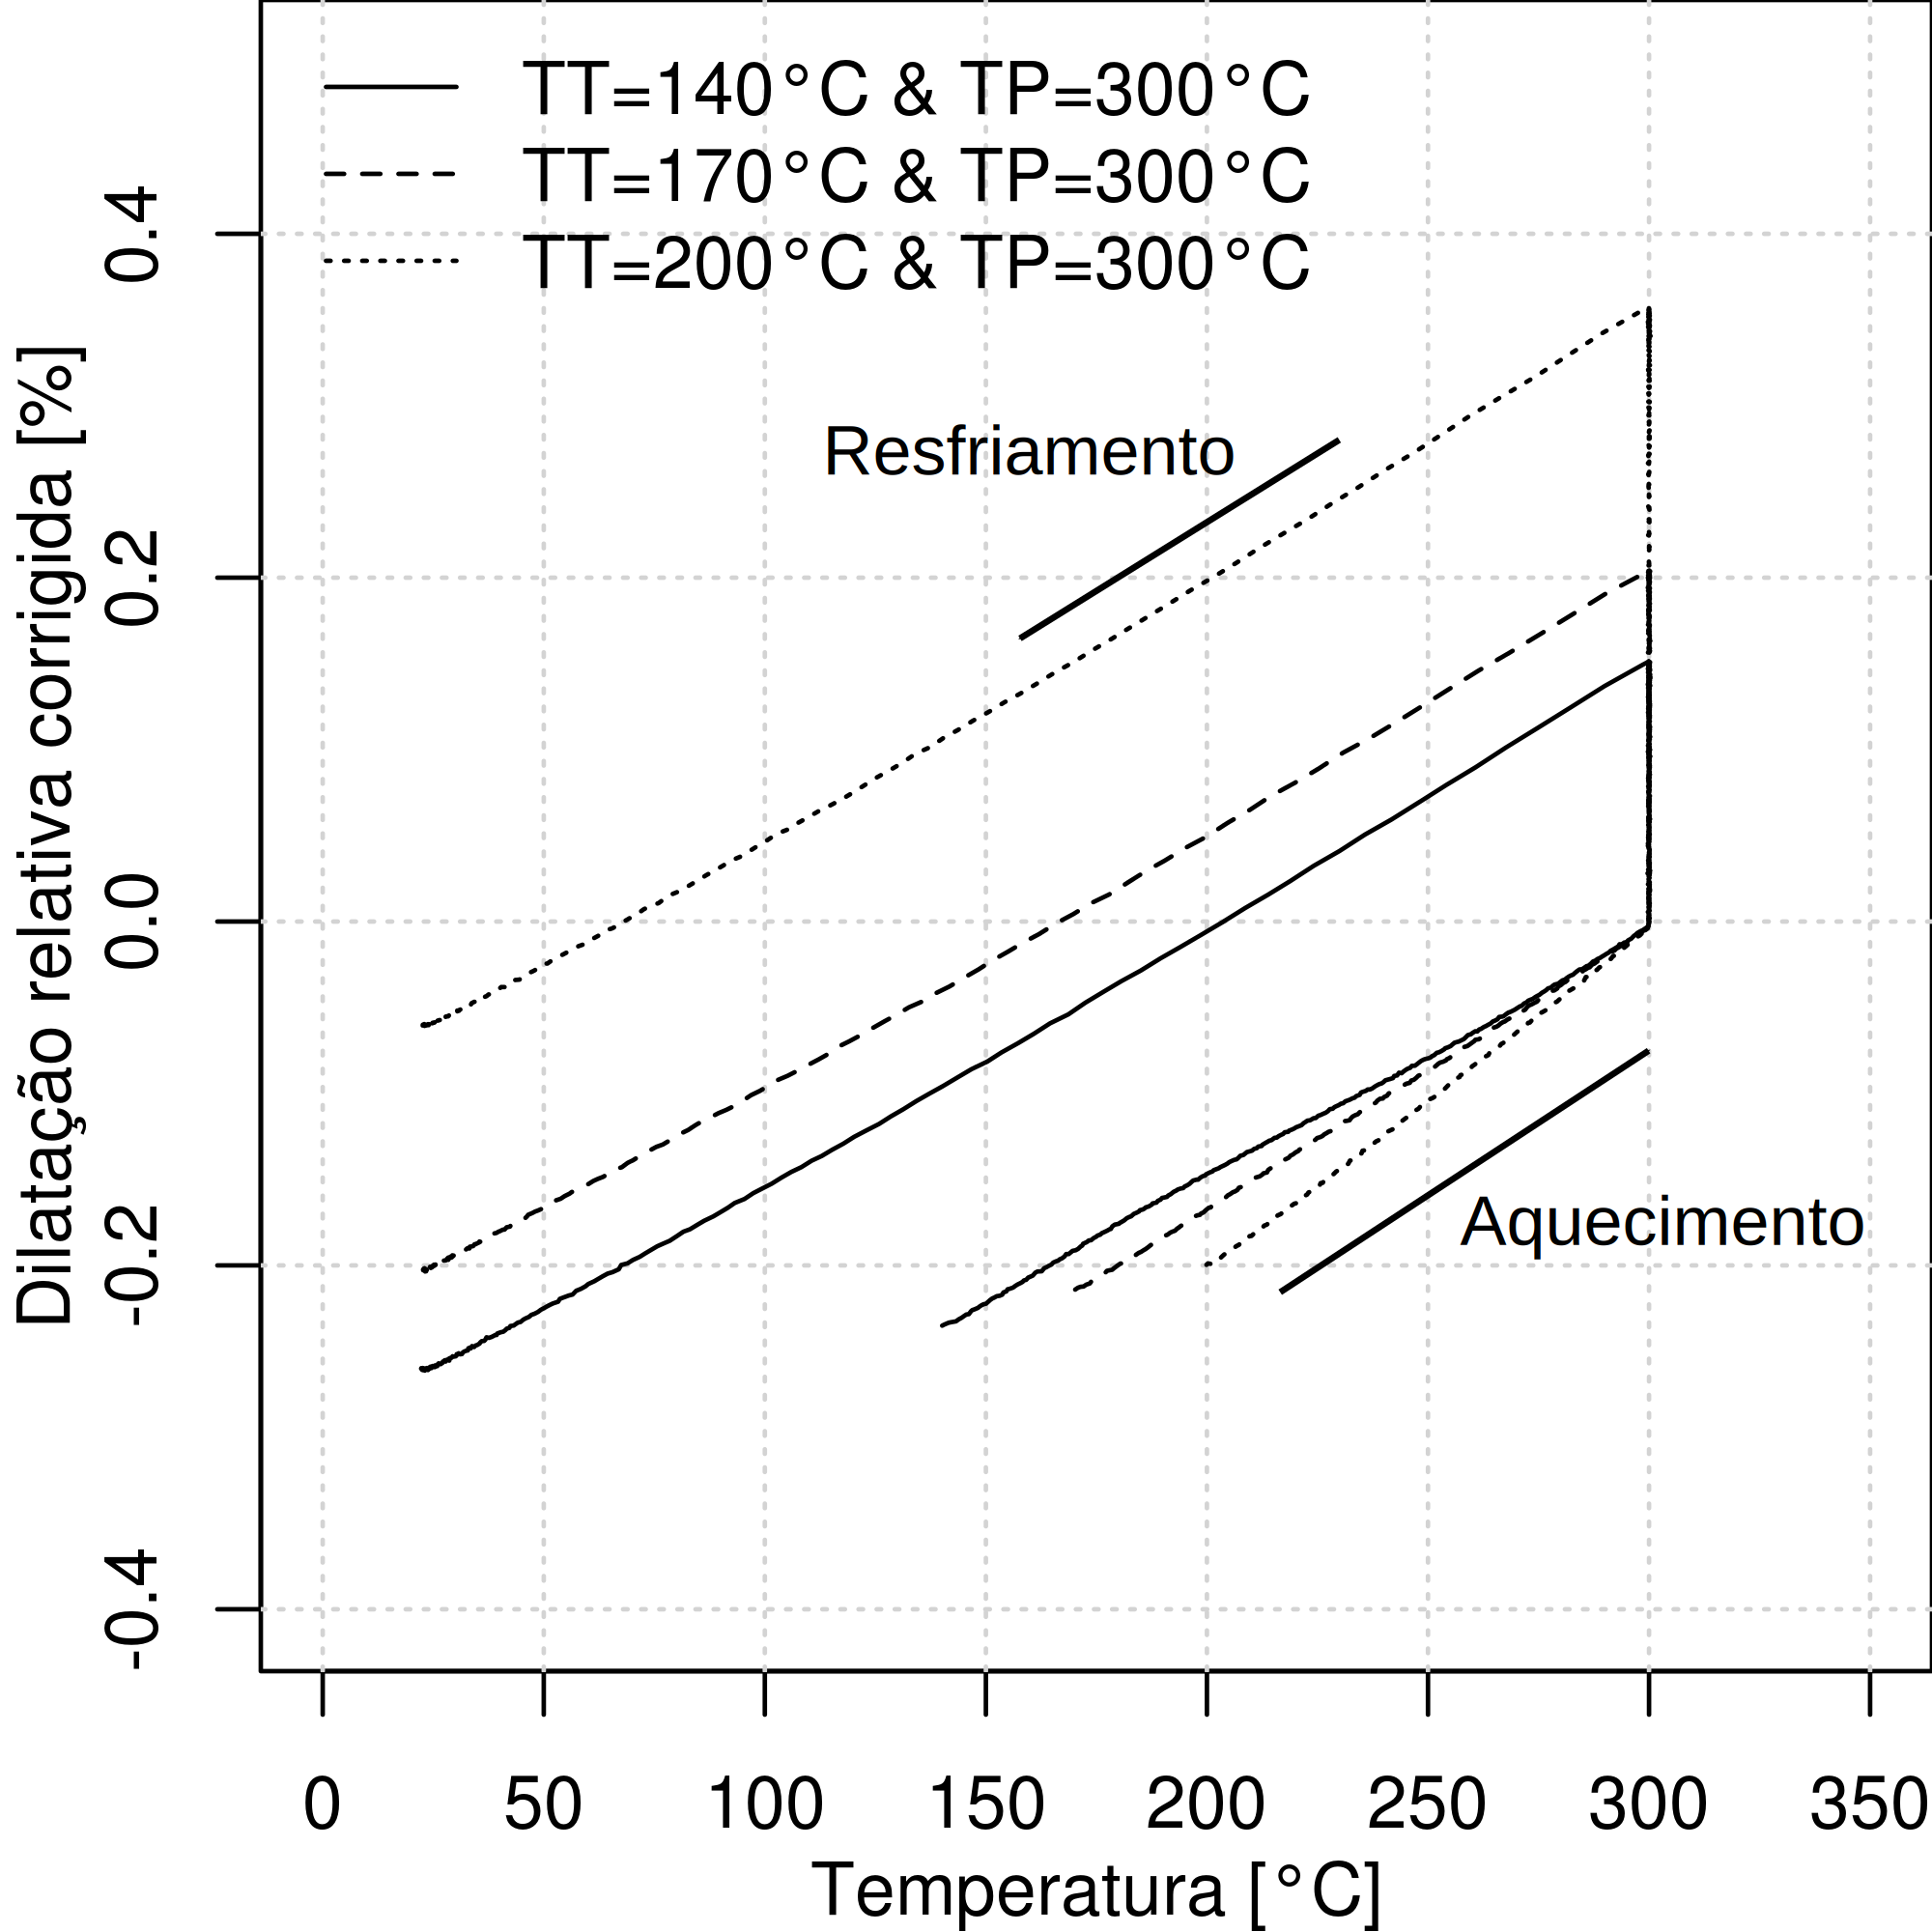
\includegraphics[width=7.5cm]{img/dilatometria/dilxT_PT300.png}}
	\caption{Curvas de dilatação das amostradas particionadas a 300 °C. (a) Dilatação relativa durante a etapa de partição em função do tempo. (b) Dilatação relativa em função da temperatura.}
	\label{fig:PT300}
\end{figure}

\begin{figure}
	\subfloat[]{\includegraphics[width=7.5cm]{img/dilatometria/dilxtime_PT375.png}}
	\quad
	\subfloat[]{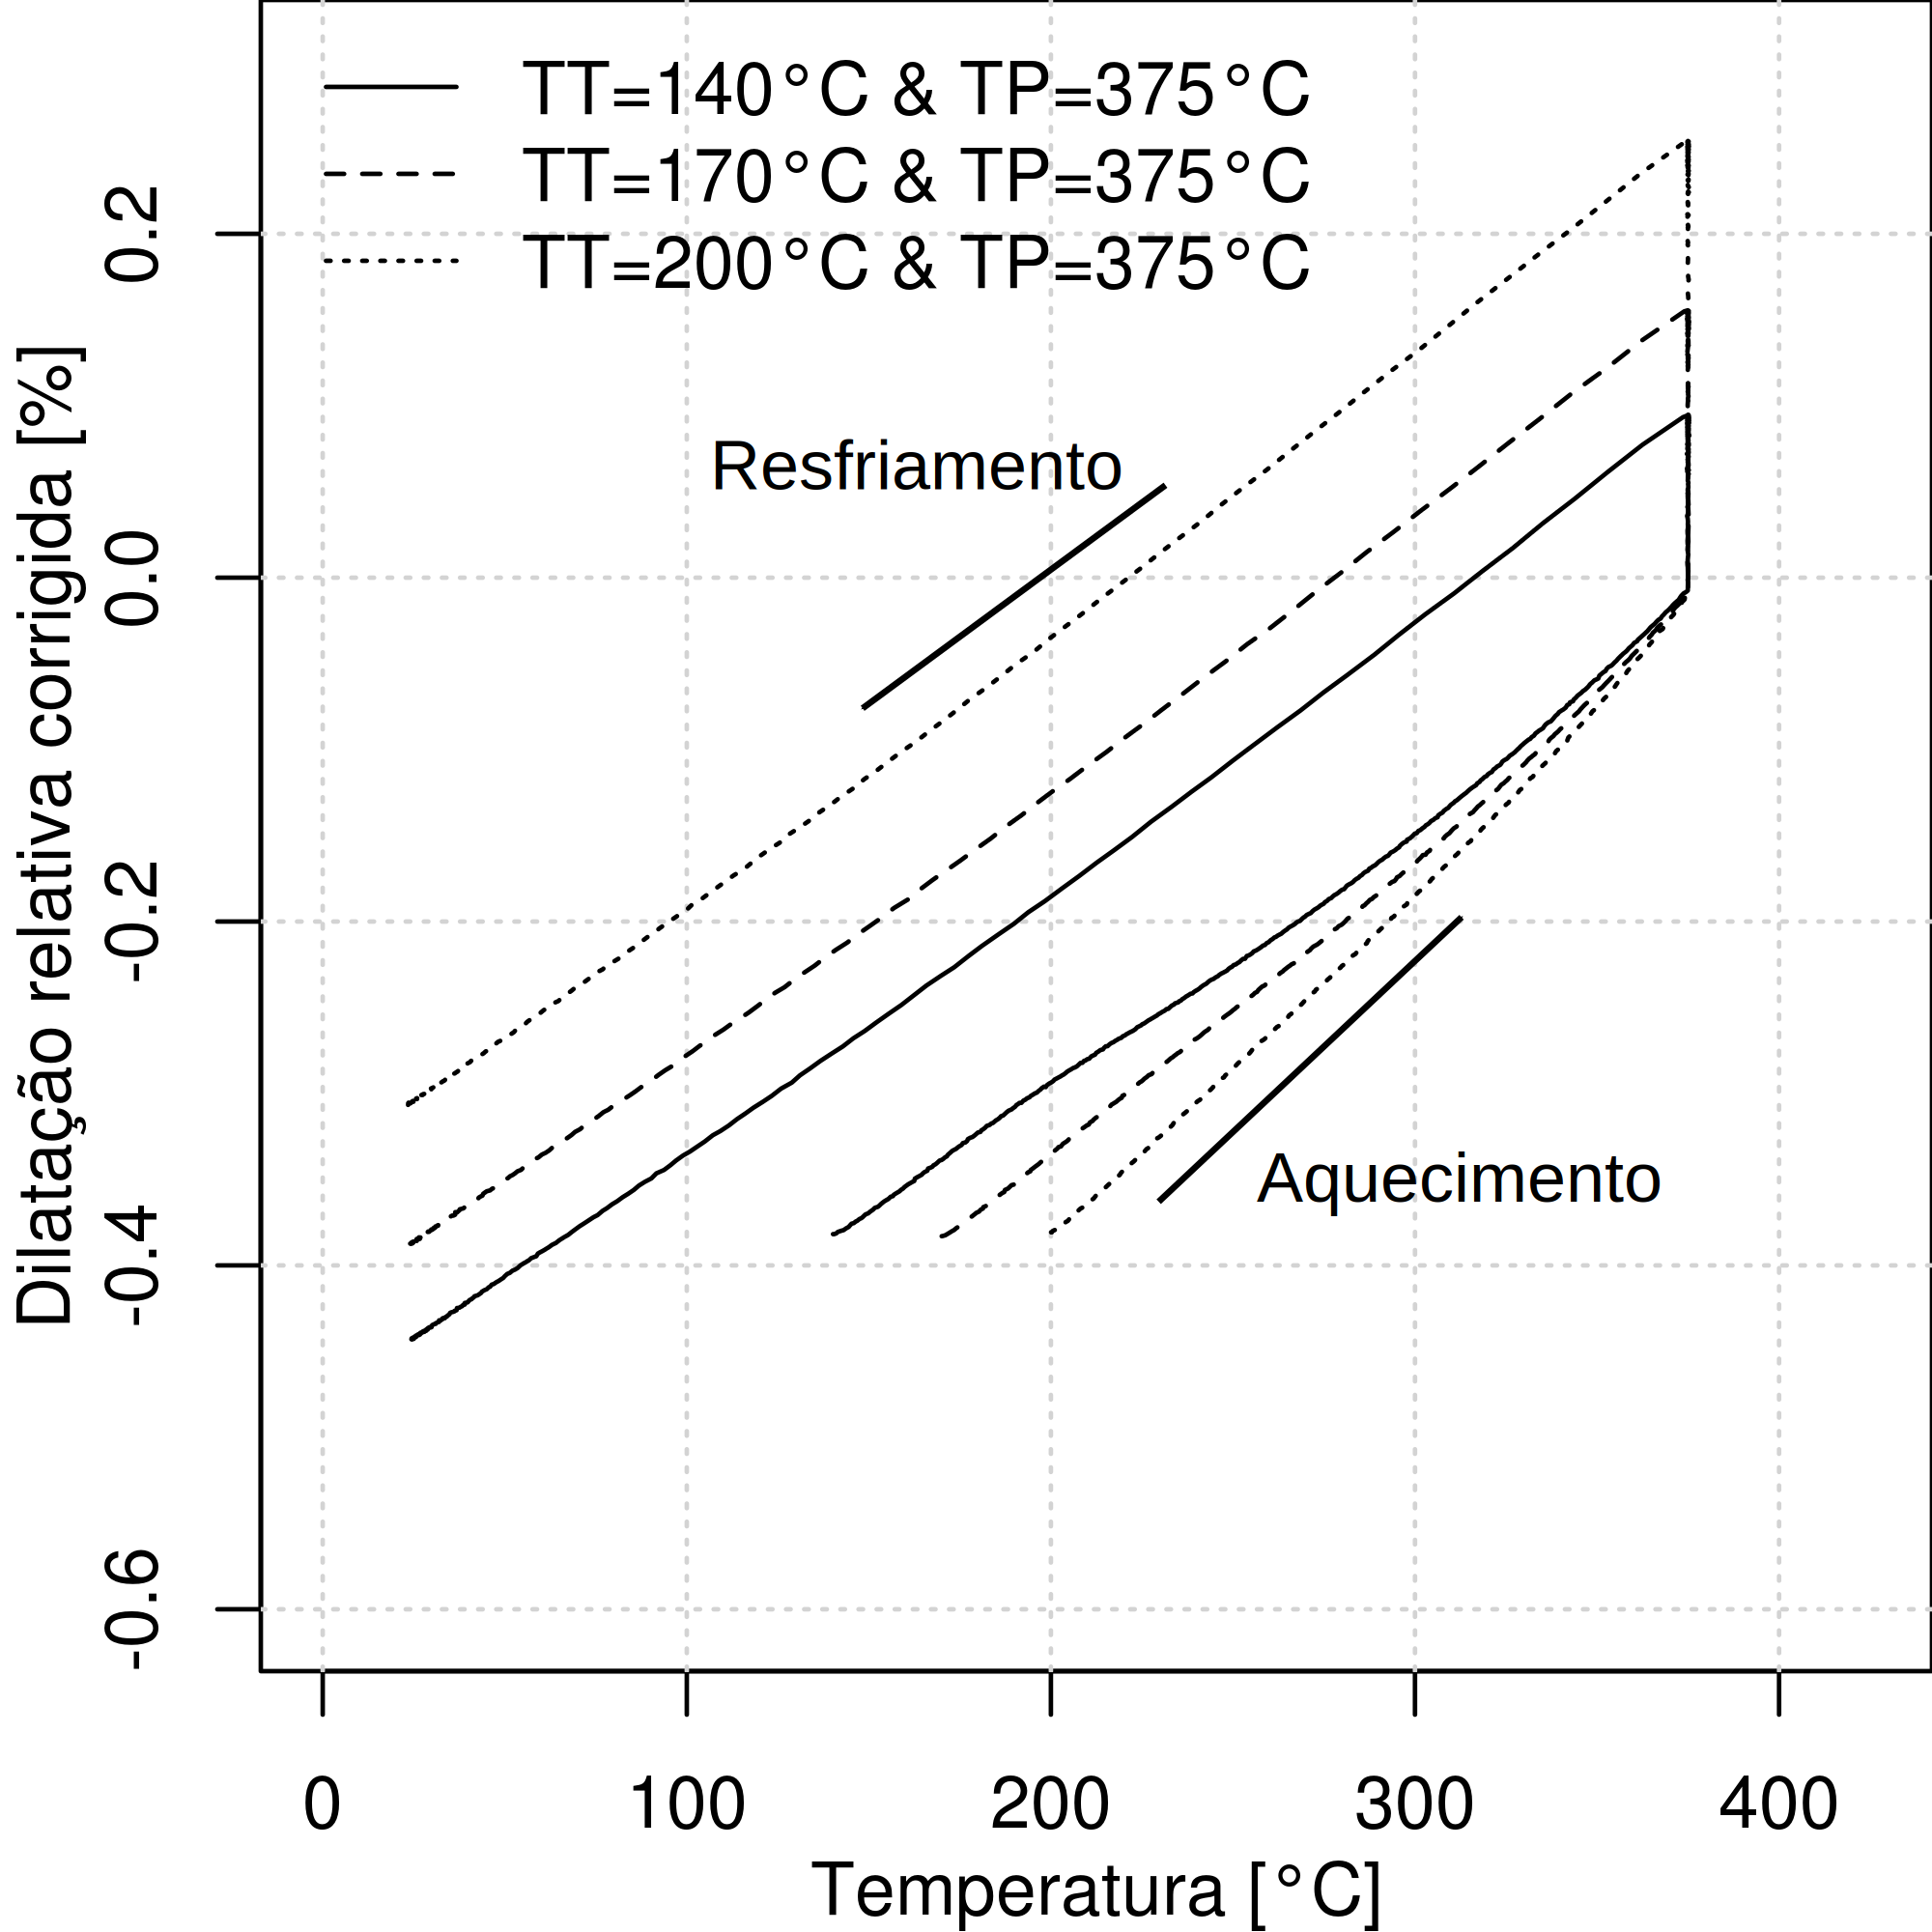
\includegraphics[width=7.5cm]{img/dilatometria/dilxT_PT375.png}}
	\caption{Curvas de dilatação das amostradas particionadas a 375 °C. (a) Dilatação relativa durante a etapa de partição em função do tempo. (b) Dilatação relativa em função da temperatura.}
	\label{fig:PT375}
\end{figure}

\begin{figure}
	\subfloat[]{\includegraphics[width=7.5cm]{img/dilatometria/dilxtime_PT450.png}}
	\quad
	\subfloat[]{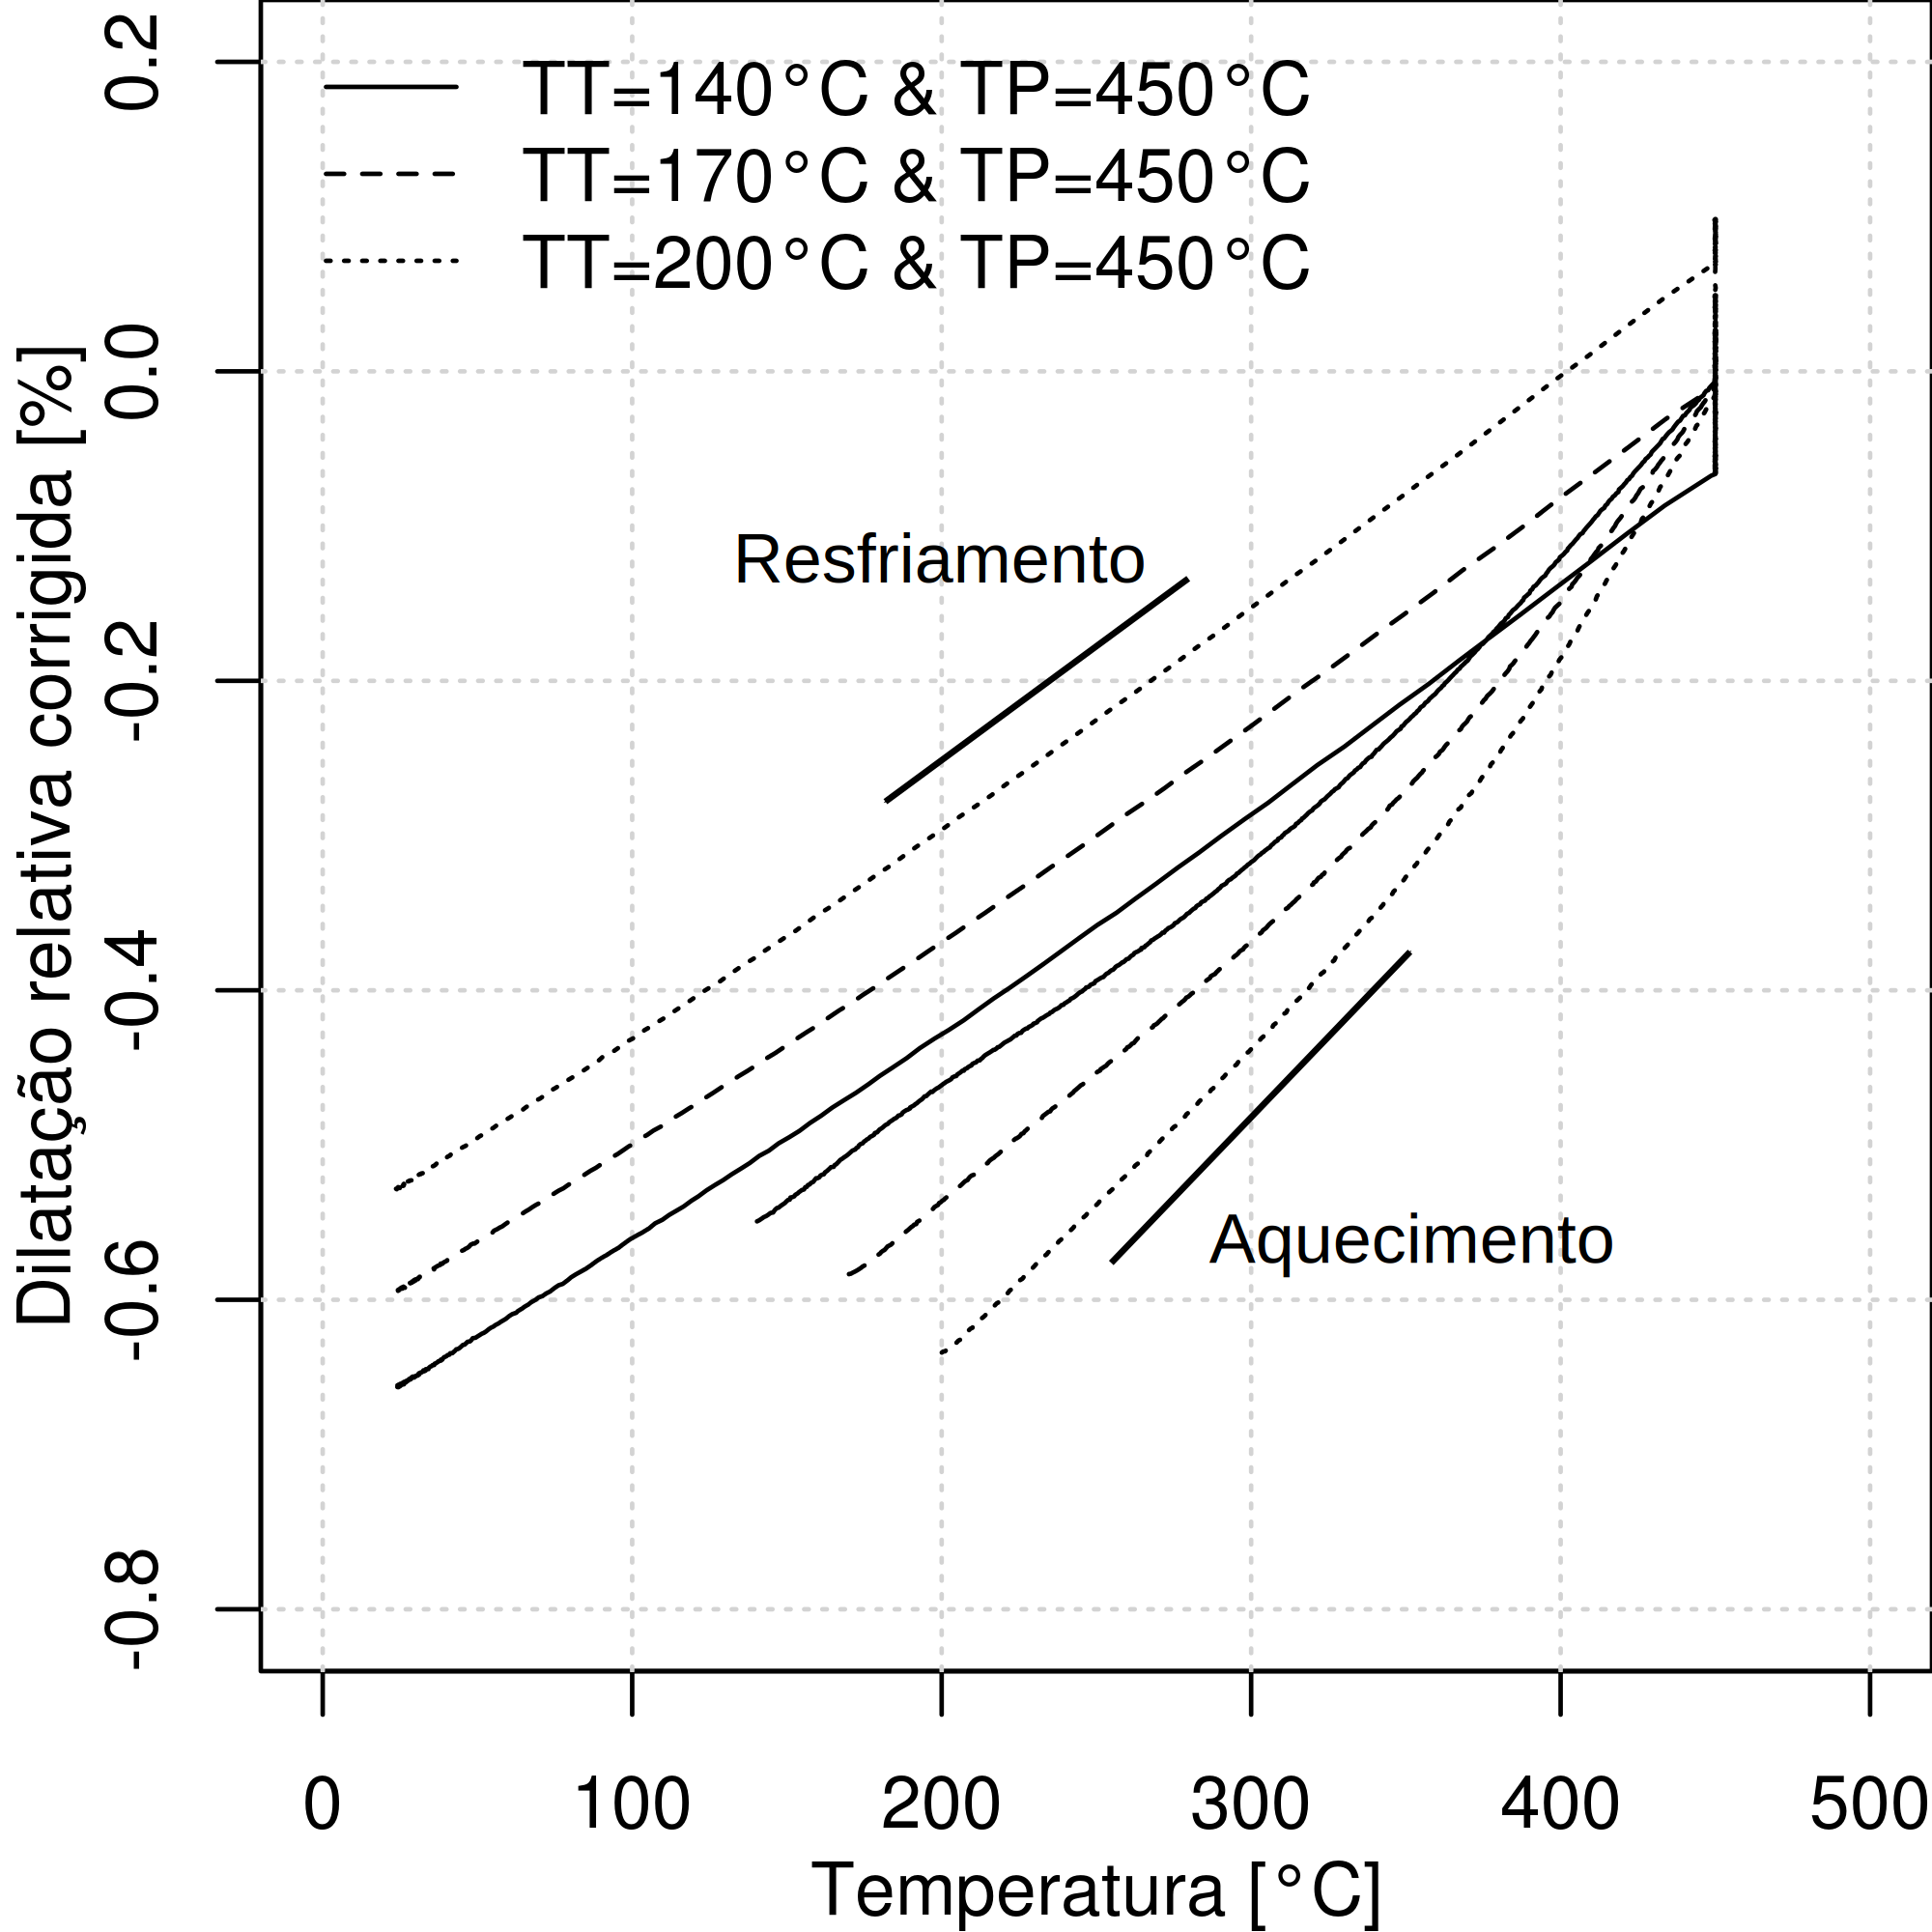
\includegraphics[width=7.5cm]{img/dilatometria/dilxT_PT450.png}}
	\caption{Curvas de dilatação das amostradas particionadas a 450 °C. (a) Dilatação relativa durante a etapa de partição em função do tempo. (b) Dilatação relativa em função da temperatura.}
	\label{fig:PT450}
\end{figure}

Mudanças no comprimento das amostras são previstas pela redistribuição de carbono da martensita para a austenita. Como pontuado na seção \ref{subsubsec:ERC}, a redistribuição de carbono segundo o modelo de equilíbrio restringido de carbono (ERC) leva a um ligeiro aumento da fração molar de austenita no material. Consequentemente, nesta situação a partição de carbono poderia vir acompanhada de uma pequena contração do material. Isto é observado apenas nas amostras particionadas a 200 °C temperadas a 140 e 170 °C (figura \ref{fig:PT200}a). Nestas amostras a contração inicial do material é procedida por uma pequena dilatação. Em todas as outras amostras há significativa expansão volumétrica durante os primeiros instantes de partição. Nas amostras particionadas a 450 °C (figura \ref{fig:PT450}) o período de expansão volumétrica é curto (cerca de 60 segundos) e no intervalo de tempo subsequente ocorre a contração das amostras.

As mudanças no comprimento das amostras particionadas em temperaturas maiores que 200 °C não podem ser explicadas pela partição de carbono segundo o modelo ERC e, portanto, são indicativos da ocorrência de reações competitivas que consomem a austenita na etapa de partição. Uma vez que as temperaturas de partição utilizadas neste trabalho são semelhantes às utilizadas no tratamento de austêmpera nos ADIs, a suspeita óbvia é que as ilhas de austenita não-transformadas são gradativamente consumidas pela reação bainítica (formação de ausferrita) durante a partição. Como nos ADIs, a reação bainítica também deve funcionar como mecanismo de enriquecimento em carbono da austenita, desde que a precipitação de carbonetos do segundo estágio da reação seja retardada.

Observa-se também uma tendência bastante clara de que temperaturas maiores têmpera levam a maiores expansões volumétricas durante a etapa de partição. Isso decorre das maiores quantidades de austenita não-transformada presentes para temperaturas maiores têmpera, disponível para decompor para o produto bainítico durante a etapa isotérmica de partição. Além disso, as amostras particionadas a 300 °C foram as que sofreram maior expansão (em torno de 0,35\% para a amostra temperada a 200 °C). Por outro lado, a contração observada durante a etapa de partição a 450 °C (figura \ref{fig:PT450}a) é tão maior quanto maior a temperatura de têmpera.

No que diz respeito ao aspecto cinético da transformação isotérmica, nota-se que as curvas de dilatação não apresentam uma etapa inicial lenta, tal qual é observada nas curvas cinéticas características previstas pelo modelo de Johnson-Mehl-Avrami-Kolmogorov (JMAK). Isso possivelmente decorre da formação de núcleos do produto bainítico durante o aquecimento desde a temperatura de têmpera até a temperatura de partição. Outra possível hipótese é que as placas de martensita formadas durante a têmpera exercem algum efeito catalizador na reação isotérmica, diminuindo a barreira de ativação para nucleação da nova fase. Hipótese semelhante foi elaborada por \citaremsentenca{Oka1988} para justificar a aceleração da reação bainítica (\textit{swing back}) em temperaturas próximas ao Ms em aços carbono.

Outra característica a ser notada é a ocorrência, durante o resfriamento final, da formação de martensita a partir da austenita que não foi suficientemente enriquecida em carbono após o término da etapa de partição. Pelas figuras \ref{fig:PT200}b e \ref{fig:PT250}b observa-se uma expansão associada à reação martensítica durante o resfriamento final nas amostras particionadas a 200 e 250 °C. Conclui-se que a austenita produzida nestas condições, de fato, não adquiriu estabilidade suficiente para ser completamente retida à temperatura ambiente. Por outro lado, nas demais amostras não foi observada expansão semelhante, ou seja, não é observada uma temperatura Ms durante o resfriamento final. Isto é associado a dois motivos: ou a austenita foi completamente estabilizada pela redistribuição de carbono durante a partição, ou a austenita foi completamente consumida pelas reações competitivas. A ocorrência de um ou outro fenômeno é discutida por meio dos resultados de difração de raios X (seção \ref{sec:DRXInSitu}).

A tabela \ref{tab:MsTP} sumariza as temperaturas Ms determinadas para cada condição estudada. Nas condições em que não houve suficiente estabilização da austenita a temperatura Ms obtida é tão maior quando menor a temperatura de têmpera. Menores temperatura de têmpera geram maiores quantidades de martensita. Nessa condição há ``mais carbono'' disponível para ser redistribuído da martensita para a austenita não transformada durante a partição. Consequentemente, a austenita particionada após a têmpera em temperaturas mais baixas acaba adquirindo um caráter mais estável do que a obtida quando a têmpera é feita em temperaturas maiores.

\begin{table}
	\caption{Temperaturas Ms determinadas para cada condição estudada após o processo T\&P.}
	\begin{tabular}{c c c ' c c c}
	\thickhline
	TT [°C] & TP [°C] & Ms [°C] & TT [°C] & TP [°C] & Ms [°C]\\
	\hline
	140 & 200 & 119 & 140 & 375 & < 25\\
	170 & 200 & 148 & 170 & 375 & < 25\\
	200 & 200 & 168 & 200 & 375 & < 25\\
	\hline
	140 & 250 & 35 & 140 & 450 & < 25\\
	170 & 250 & 77 & 170 & 450 & < 25\\
	200 & 250 & 109 & 200 & 450 & < 25\\
	\hline
	140 & 300 & < 25 &&&\\
	170 & 300 & < 25 &&&\\
	200 & 300 & < 25 &&&\\
	\thickhline
	\end{tabular}
	\label{tab:MsTP}
\end{table}

Assumindo que a diminuição da temperatura Ms é consequente do enriquecimento em carbono da austenita, é possível estimar o acréscimo $\Delta \%w_C^\gamma$ em carbono da austenita durante a etapa de partição pela equação de Andrews (equação \ref{eq:Andrews}). Nesta equação, o coeficiente de valor 423 que acompanha a variável $\%w_C^\gamma$ significa que o aumento de 1\% no teor de carbono da austenita provoca a diminuição de 423 °C na temperatura Ms desta fase. Com base nesse raciocínio, a tabela \ref{tab:wCgammaAndrews}, sumarizando os valores de $\Delta \%w_C^\gamma$ para as condições de tratamento térmico foi obtida.

\begin{table}
	\caption{Estimativa da variação no teor de carbono da austenita ($\Delta \%w_C^\gamma$) após o processo T\&P para cada condição de tratamento térmico.}
	\begin{tabular}{c c c ' c c c}
	\thickhline
	TT [°C] & TP [°C] & $\Delta \%w_C^\gamma$ & TT [°C] & TP & $\Delta \%w_C^\gamma$\\
	\hline
	140 & 200 & 0,26 & 140 & 375 & > 0,48\\
	170 & 200 & 0,19 & 170 & 375 & > 0,48\\
	200 & 200 & 0,15 & 200 & 375 & > 0,48\\
	\hline
	140 & 250 & 0,46 & 140 & 450 & > 0,48\\
	170 & 250 & 0,36 & 170 & 450 & > 0,48\\
	200 & 250 & 0,29 & 200 & 450 & > 0,48\\
	\hline
	140 & 300 & > 0,48 &&&\\
	170 & 300 & > 0,48 &&&\\
	200 & 300 & > 0,48 &&&\\
	\thickhline
	\end{tabular}
	\label{tab:wCgammaAndrews}
\end{table}

\subsection{Resposta dilatom\'{e}trica durante ciclos t\'{e}rmicos de aust\^{e}mpera}

Uma vez que foram observadas expansões volumétricas significativas durante a etapa de partição do processo T\&P e foi levantada a hipótese de que estas variações no comprimento estariam associadas a reações semelhantes às observadas durante a produção de ADIs, tratamentos isotérmicos de austêmpera foram realizados para se determinar o comportamento cinético da reação bainítica no ferro nodular estudado. A figura \ref{fig:IBT} ilustra este comportamento durante o patamar isotérmico de austêmpera.

\begin{figure}
	\includegraphics[height=12cm]{img/dilatometria/dilation_IBT.png}
	\caption{Curvas de dilatação das amostradas tratadas isotermicamente entre 200 e 450 °C.}
	\label{fig:IBT}
\end{figure}

Observa-se que em todas as condições estudadas há sensível expansão das amostras. Com exceção das amostras austemperadas a 200 °C, pode-se concluir em todas as condições as curvas dilatométricas apresentaram um formato sigmoidal característico, compatível com a descrição cinética prevista pela equação de JMAK. Isto é interpretado pela lenta cinética no começo da transformação, associada à etapa de nucleação da fase produto, procedida por uma rápida expansão, relacionada ao crescimento do produto bainítico.

Dentre as amostras tratadas entre 300 e 450 °C, menores temperaturas de tratamento isotérmico produziram maiores expansões volumétricas dos corpos de prova. Isto é justificado pela diferença entre os valores dos coeficientes de expansão térmica da austenita e da ferrita, maior para a primeira a fase. Como pode ser observado na figura \ref{fig:dilRel}, estas diferenças afetam a dilatação produzida pela formação da ferrita (fase cúbica de corpo centrado) a partir da austenita (fase cúbica de face centrada). A mesma justificativa pode ser utilizada para explicar os resultados obtidos nas amostras tratadas pelo processo T\&P.

\begin{figure}
	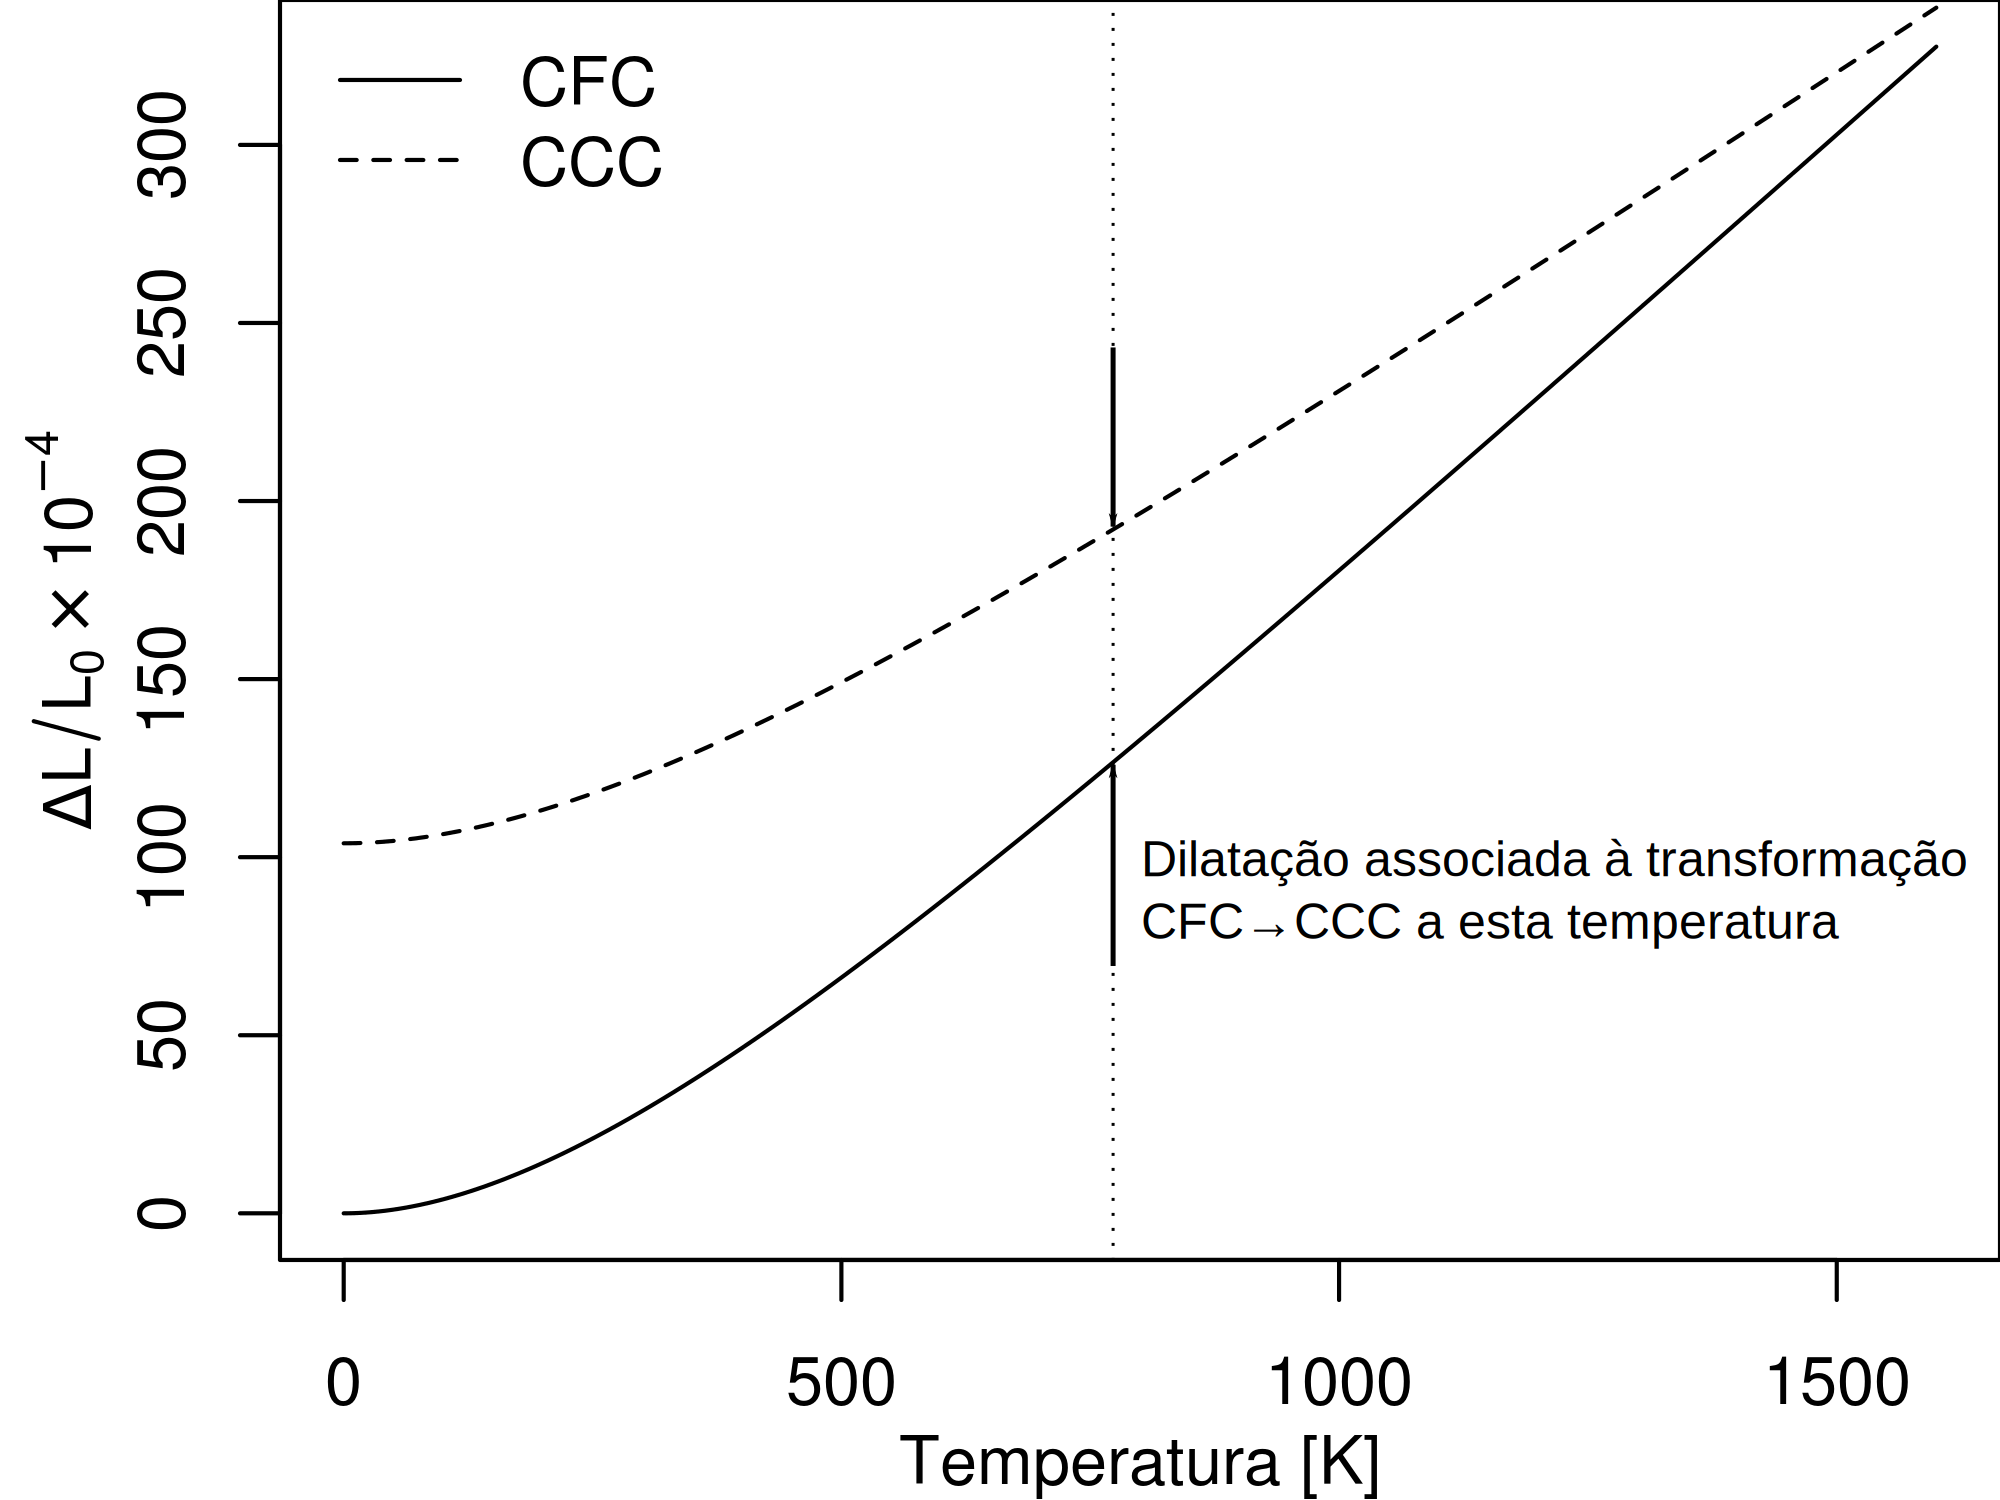
\includegraphics[width=12cm]{img/dilation_alphagamma.png}
	\caption{Dilatação térmica relativa ($\Delta L/L_0$) das fases cúbica de corpo centrado (CCC) e cúbica de corpo centrado (CFC). Curvas calculadas por meio das equações empíricas obtidas por\cite{VanBohemen2013b}.}
	\label{fig:dilRel}
\end{figure}

O tratamento de austêmpera da amostra tratada a 200 °C é essencialmente o mesmo aplicado no processo T\&P nas temperaturas de têmpera e partição de 200 °C. Nessa situação, a forte expansão observada no início do tratamento térmico é decorrente da transformação martensítica, haja vista esta temperatura de austêmpera é inferior à temperatura Ms. A dilatação subsequente, no entanto, não é completamente compatível com modelo JMAK e pode ser associada à partição de carbono da martensita para a austenita, precipitação de carbonetos no interior da martensita, ou mesmo a ocorrência da decomposição da austenita abaixo da temperatura Ms.

A amostra austemperada a 450 °C não apresentou contração durante a etapa isotérmica, ao contrário das amostras temperadas e particionadas na mesma temperatura. Dessa forma, descarta-se a hipótese de que a contração volumétrica nas amostras submetidas ao ciclo têmpera e partição a 450 °C esteja associada à reação bainítica durante a etapa de partição e devem estar associadas à precipitação de carbonetos no revenimento da martensita. Isso é compatível com a literatura sobre o assunto, que indica que tanto a precipitação de carbonetos de transição, quanto a precipitação da cementita levam à contração do material\cite{Morra2001}.

\section{Difra\c{c}\~{a}o de raios X \textit{in situ}}

\label{sec:DRXInSitu}

O mapa de cores da figura \ref{fig:colorMap} mostra a evolução dos padrões de difração ao etapa de partição da amostra temperada a 170 °C e particionada a 300 °C. Nesta figura as tonalidades representam a raiz quadrada da intensidade das reflexões do experimento de difração. É possível observar a evolução de diferentes picos associados ao obedecimento das condições de difração da austenita (fase $\gamma$) e da ferrita/martensita (fase $\alpha$).

\begin{figure}
	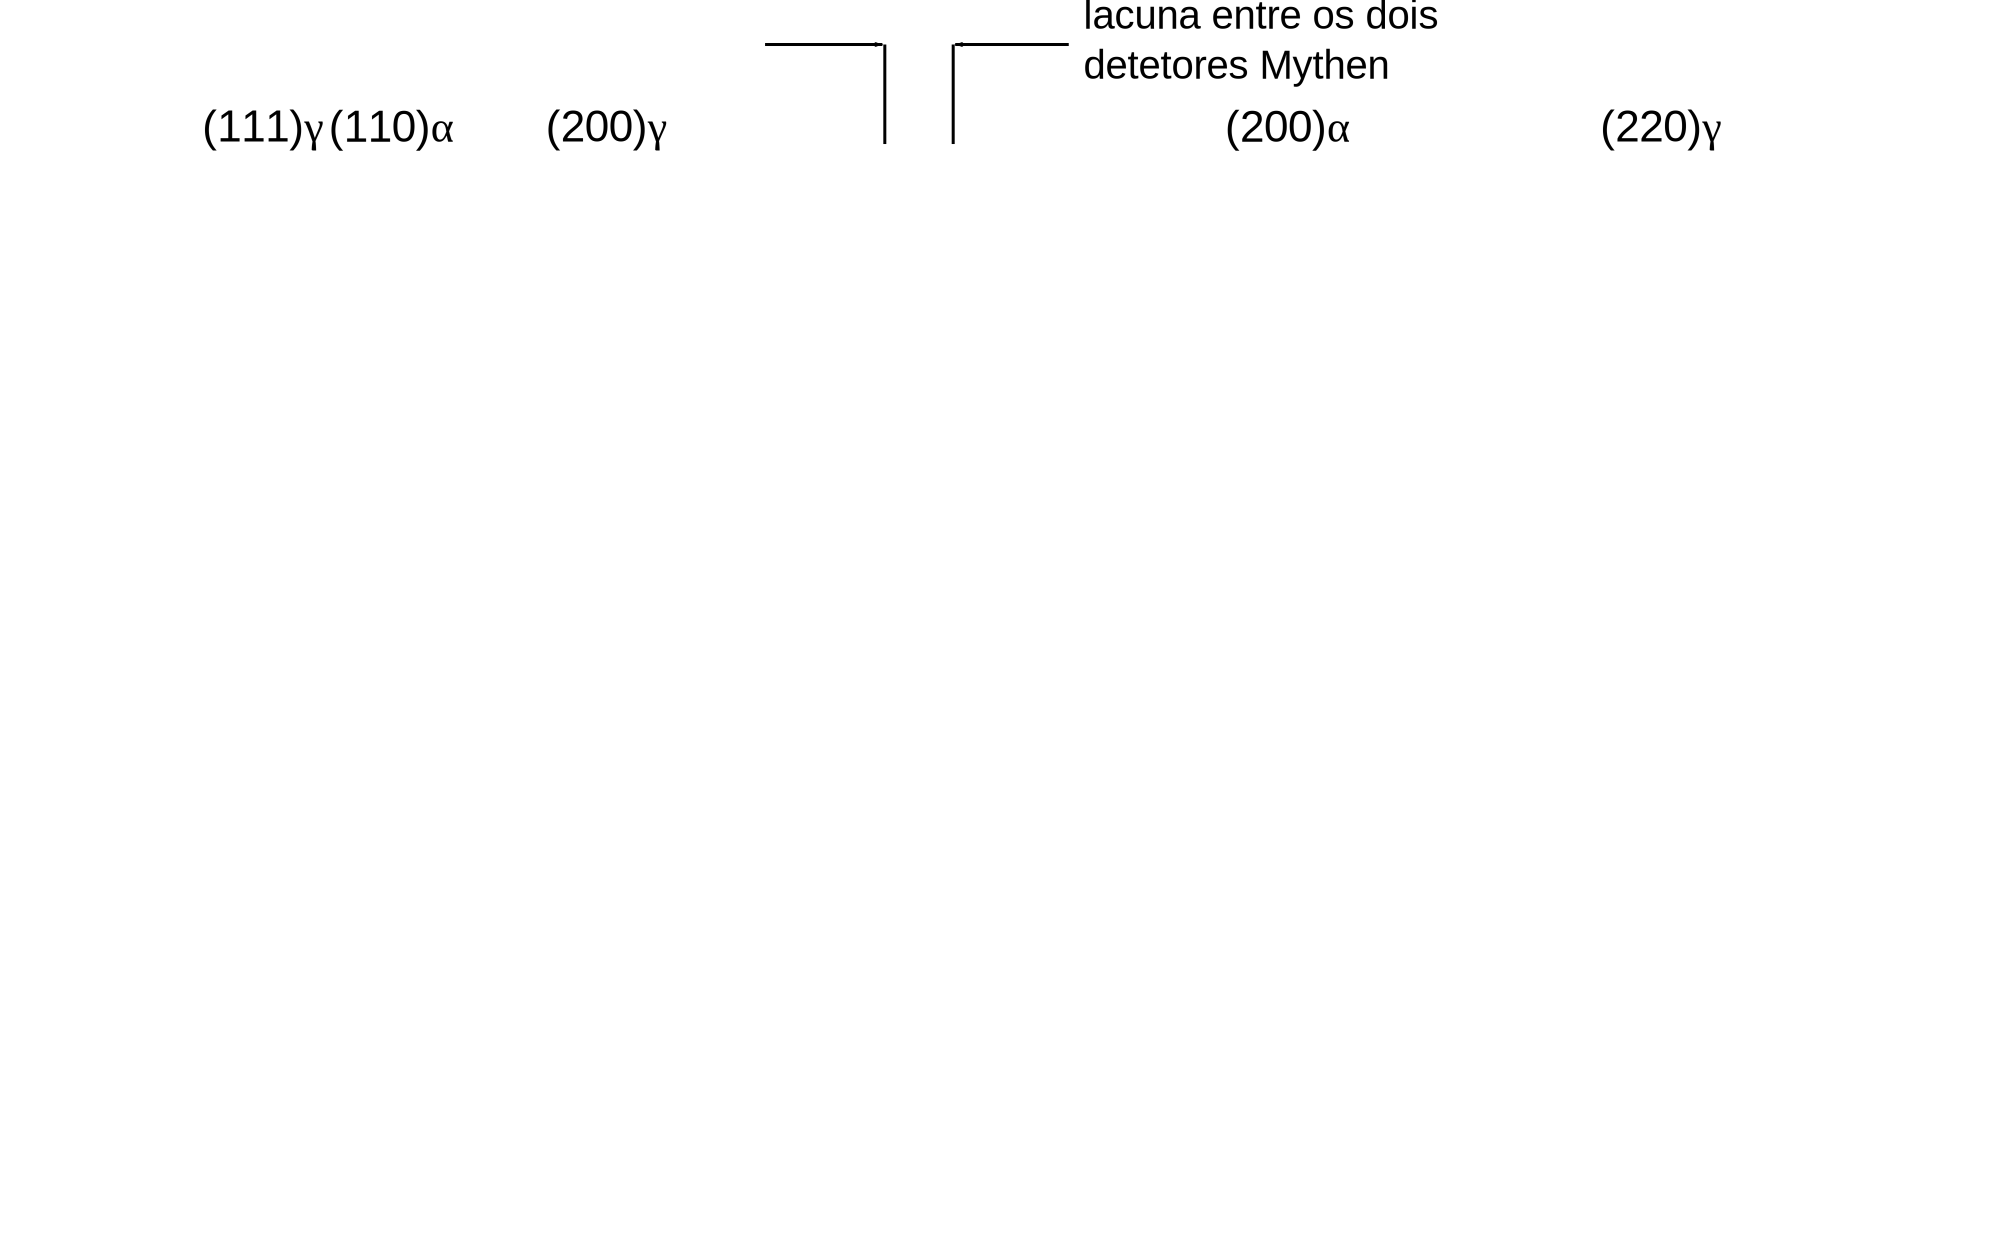
\includegraphics[width=16cm]{img/XTMS/map_TT170TP300.png}
	\caption{Mapa de cores representado a evolução dos picos de difração da austenita ($\gamma$) e da ferrita ($\alpha$) ao longo da etapa de partição. No eixo das abscissas é representado o ângulo de difração $2\theta$, enquanto no eixo das ordenadas é representado o tempo de partição em segundos. As tonalidades de cores correspondem à raiz quadrada da intensidade segundo a escala mostrado ao lado do mapa.}
	\label{fig:colorMap}
\end{figure}

Na figura \ref{fig:colorMap2} é possível ver em detalhe o mapa de cores da figura \ref{fig:colorMap}. É possível observar dois principais comportamentos: o deslocamento do pico {111} da austenita para ângulos menores de difração e sua diminuição de intensidade ao longo da etapa de partição. A lei de Bragg (equação \ref{eq:Bragg}) prevê que valores menores do ângulo $2\theta$ estão associados a maiores distâncias interplanares e, consequentemente, a maiores parâmetros de rede. Por sua vez, o aumento do parâmetro de rede é associado ao enriquecimento em carbono da austenita. A diminuição da intensidade do pico da austenita é interpretado pelo consumo da fase por uma reação competitiva, confirmando os resultados de dilatometria.

\begin{figure}
	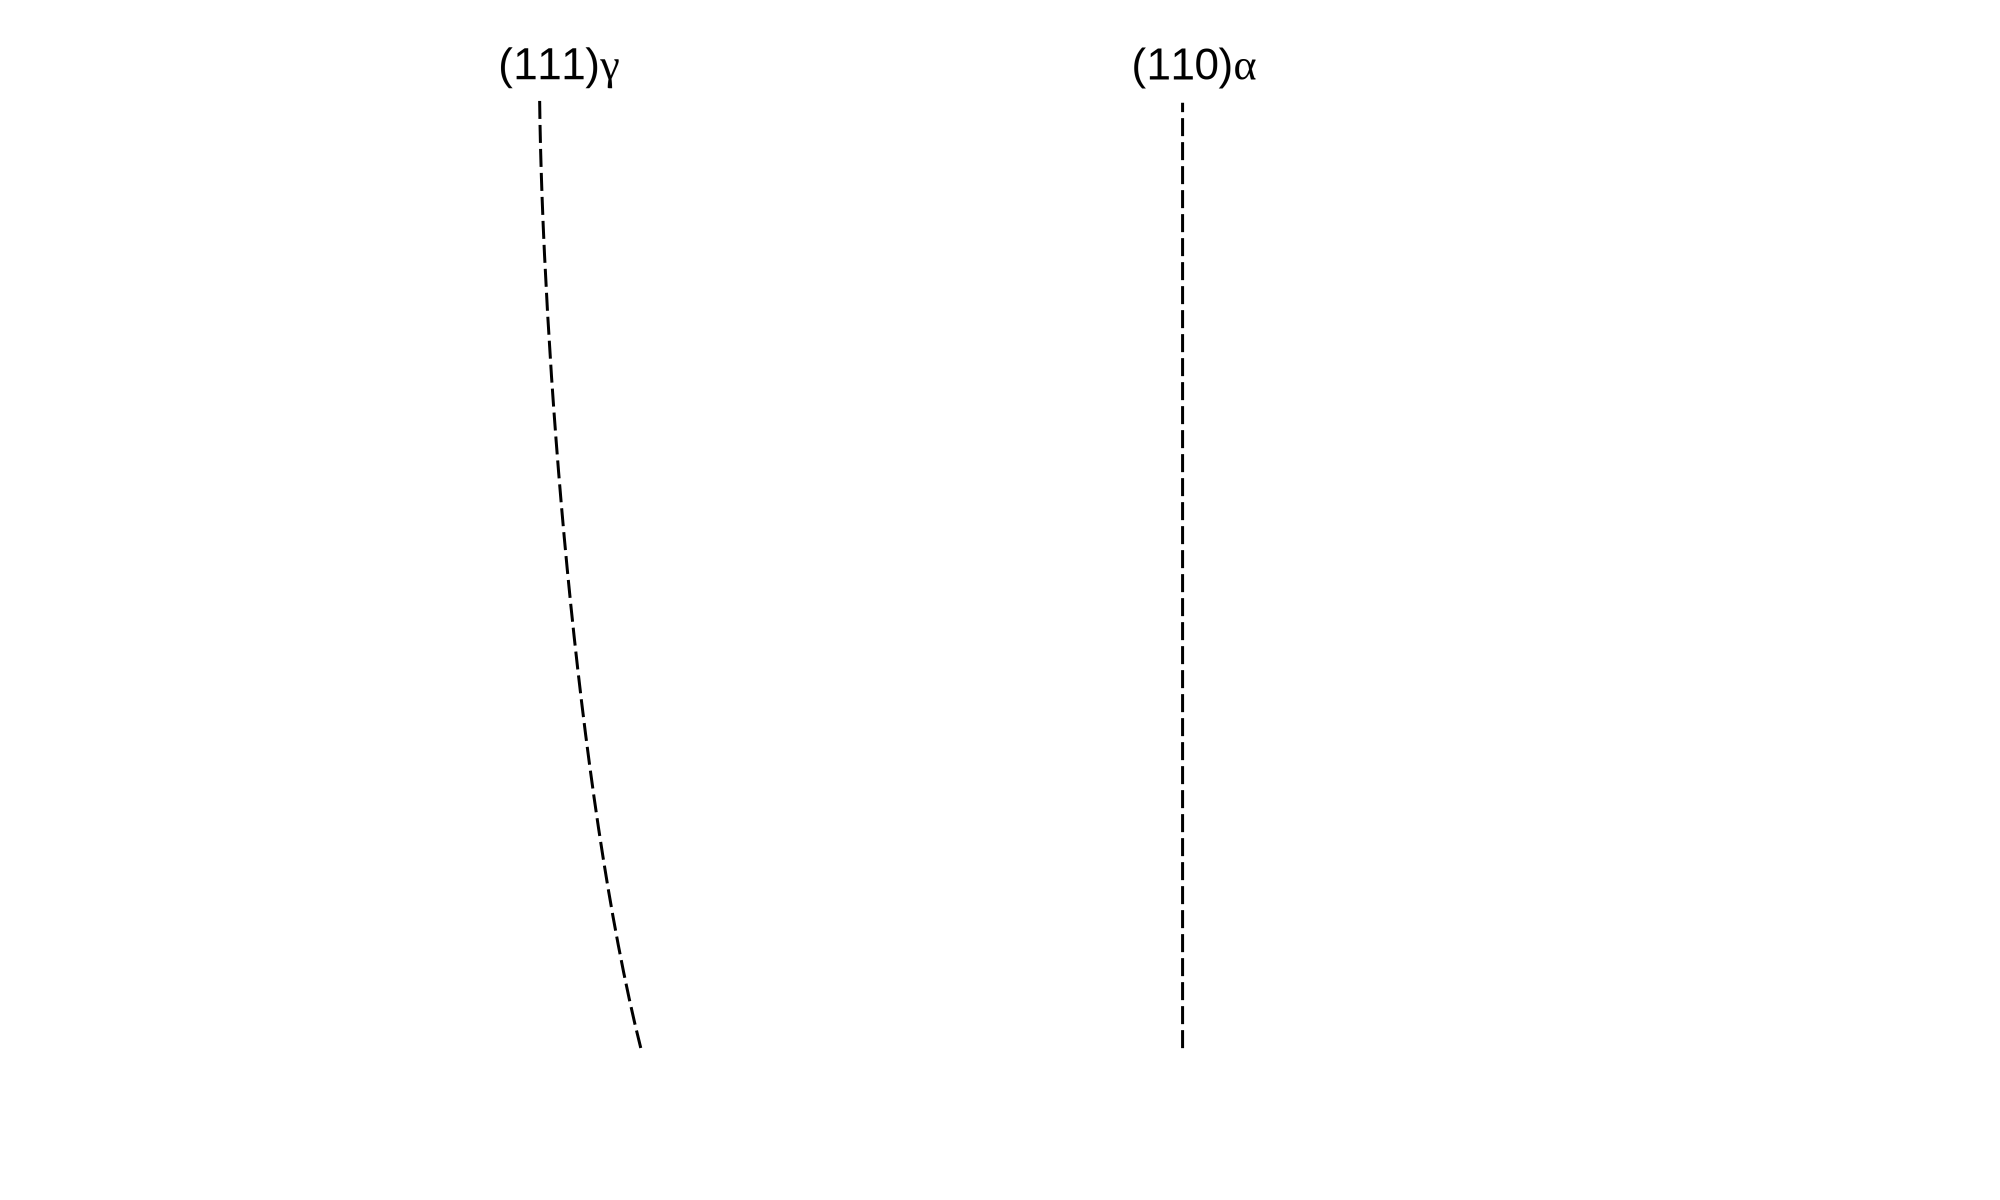
\includegraphics[width=16cm]{img/XTMS/map_TT170TP300_2.png}
	\caption{Detalhe do mapa de cores mostrado na figura \ref{fig:colorMap}.}
	\label{fig:colorMap2}
\end{figure}

As figuras \ref{fig:XTMSPT200} a \ref{fig:XTMSPT450} mostram os resultados de difração tratados para determinação da fração do produto isotérmico ($f^{\alpha\text{-iso}}$) formado durante a etapa de partição e a variação do teor de carbono dissolvido na austenita ($\Delta\%w_C^\gamma$), obtido pela relação de Dyson e Holmes (equação \ref{eq:parametroRede}).

\begin{figure}
	\subfloat[]{\includegraphics[width=7.5cm]{img/XTMS/f_isoPT200.png}}
	\quad
	\subfloat[]{\includegraphics[width=7.5cm]{img/XTMS/wC_gamma200.png}}
	\caption{Fração volumétrica do produto isotérmico formado durante a partição (a) e teor de carbono dissolvido na austenita (b) para as amostradas particionadas a 200 °C.}
	\label{fig:XTMSPT200}
\end{figure}

\begin{figure}
	\subfloat[]{\includegraphics[width=7.5cm]{img/XTMS/f_isoPT250.png}}
	\quad
	\subfloat[]{\includegraphics[width=7.5cm]{img/XTMS/wC_gamma250.png}}
	\caption{Fração volumétrica do produto isotérmico formado durante a partição (a) e teor de carbono dissolvido na austenita (b) para as amostradas particionadas a 250 °C.}
	\label{fig:XTMSPT250}
\end{figure}

\begin{figure}
	\subfloat[]{\includegraphics[width=7.5cm]{img/XTMS/f_isoPT300.png}}
	\quad
	\subfloat[]{\includegraphics[width=7.5cm]{img/XTMS/wC_gamma300.png}}
	\caption{Fração volumétrica do produto isotérmico formado durante a partição (a) e teor de carbono dissolvido na austenita (b) para as amostradas particionadas a 300 °C.}
	\label{fig:XTMSPT300}
\end{figure}

\begin{figure}
	\subfloat[]{\includegraphics[width=7.5cm]{img/XTMS/f_isoPT375.png}}
	\quad
	\subfloat[]{\includegraphics[width=7.5cm]{img/XTMS/wC_gamma375.png}}
	\caption{Fração volumétrica do produto isotérmico formado durante a partição (a) e teor de carbono dissolvido na austenita (b) para as amostradas particionadas a 375 °C.}
	\label{fig:XTMSPT375}
\end{figure}

\begin{figure}
	\subfloat[]{\includegraphics[width=7.5cm]{img/XTMS/f_isoPT450.png}}
	\quad
	\subfloat[]{\includegraphics[width=7.5cm]{img/XTMS/wC_gamma450.png}}
	\caption{Fração volumétrica do produto isotérmico formado durante a partição (a) e teor de carbono dissolvido na austenita (b) para as amostradas particionadas a 450 °C.}
	\label{fig:XTMSPT450}
\end{figure}

Observam-se comportamentos semelhantes aos constatados nos resultados de dilatometria. Nota-se que, dentre as amostras particionadas a 200 °C, há, de fato, a formação de uma pequena quantidade do produto $\alpha\text{-iso}$ na amostra temperada a 200 °C(figura \ref{fig:XTMSPT200}a). No entanto, o enriquecimento em carbono da austenita é praticamente imperceptível pela análise das curvas da figura \ref{fig:XTMSPT200}b. Esse resultado vai contra a observação feita pelos resultados de dilatometria de que mesmo nas condições partição a 200 °C a temperatura Ms diminui consideravelmente (vide tabela \ref{tab:MsTP}).

Nas demais condições de tratamento térmico também é possível observar substancial aumento da fração volumétrica da fase cúbica de corpo centrado ($\alpha$) e consequente diminuição da fração volumétrica da austenita não transformada. Confirmando os resultados apontados pela dilatometria, maiores temperaturas de têmpera produziram maiores frações do produto isotérmico. Em contrapartida, com exceção das amostras particionadas a 450 °C, o enriquecimento em carbono da austenita também é significativo. Além disso, o comportamento das curvas de variação do carbono na austenita é bastante similar às curvas de fração transformada. Isso leva à conclusão de que a formação do produto isotérmico $\alpha\text{-iso}$ contribui fortemente para o enriquecimento em carbono e estabilização da austenita.

Nas amostras particionadas a 300 °C, após os 15 minutos da etapa de partição todas as condições de têmpera produziram aproximadamente o mesmo acréscimo no teor de carbono de austenita, cerca de 0,6\% (figura \ref{fig:XTMSPT300}b). O que se mostra diferente entre as três diferentes condições de têmpera é o comportamento cinético nos primeiros segundos da etapa de partição: a amostra temperada a 140 °C leva ao enriquecimento em carbono da austenita de forma mais rápida do que nas demais condições. Esse resultado complementa a análise feita com os resultados de dilatometria. Parece razoável concluir que a quantidade de martensita formada durante a etapa de têmpera --- tão maior, quanto menor a temperatura de têmpera --- desempenha papel fundamental na cinética da reação isotérmica.

As amostras particionadas a 375 °C não apresentam a mesma convergência do teor de carbono na austenita após a etapa de partição. A condição de têmpera a 170 °C produziu cerca de 0,7\% de acréscimo no teor de carbono da austenita, contra 0,6\% obtido para a amostra temperada a 140 °C. Nessa situação, diferenças no comportamento cinético não foram observadas.

Nas amostras tratadas a 450 °C observa-se uma descontinuidade nas curvas de fração transformada (figura \ref{fig:XTMSPT450}a). Isto é consequente da dificuldade da rotina numérica quantificar as quantidades muito pequenas de austenita restantes no final da etapa de partição. Esta foi a única condição de partição que levou ao consumo completo da austenita ao final da etapa de partição. Por este motivo, o teor de carbono dissolvido na austenita gerou resultados bastante ruidosos para os instantes finais de partição (figura \ref{fig:XTMSPT450}b). Dessa forma, embora se observe uma aparente diminuição no teor de carbono da austenita ao final da partição, esta conclusão pode estar sendo prejudicada pelo método de medição em si.

\subsection{Carbono dissolvido na martensita particionada/ferrita formada isotermicamente}

\label{subsec:wCalpha}

Assumindo que as únicas fases presente na matriz do ferro fundido são a austenita $\gamma$ e a martensita particionada/ferrita isotérmica $\alpha$, o teor de carbono médio dissolvido na fase $\alpha$ pode ser determinado a partir dos resultados de DRX utilizando as equações de balanço de massa de carbono e de balanço das quantidades das fases:

\begin{subequations}
	\begin{align}
		&\%w_C^\alpha \cdot f^\alpha + \%w_C^\gamma \cdot f^\gamma = \%w_C^0\\
		&f^\alpha + f^\gamma = 1 
	\end{align}
	\label{eq:wCalpha}
\end{subequations}
%
em que $w_C^\alpha$ e $w_C^\gamma$ são as porcentagens em massa de carbono dissolvido nas fases $\alpha$ e $\gamma$, respectivamente, $w_C^0$ é o teor de carbono inicial dissolvido na austenita e $f^\alpha$ e $f^\gamma$ são as frações volumétricas de $\alpha$ e $\gamma$. A partir das equações acima e, assumindo o teor de carbono inicial da austenita determinado pelos cálculos termodinâmicos pelo Thermo-Calc\textregistered{} (0,76\%, segundo a tabela \ref{tab:CQaust}, a evolução do teor de carbono na ferrita/martensita ao longo da etapa de partição foi determinada para cada condição estudada, sendo mostrada na figura \ref{fig:wCalpha}.

\begin{figure}
	\includegraphics[width=12cm]{img/XTMS/wC_alpha.png}
	\caption{Teor de carbono dissolvido na ferrita/martensita em função do tempo de partição.}
	\label{fig:wCalpha}
\end{figure}

Nota-se que nas condições de partição a 450 °C há uma inicial diminuição do carbono na fase $\alpha$, seguida de um rápido aumento, até o reestabelecimento da fração inicial de carbono. Esse resultado é incompatível com a segunda lei da termodinâmica, pois o enriquecimento em carbono da ferrita ao longo de um tratamento isotérmico provocaria o aumento da energia livre do sistema. O que acontece nesta situação é que, como as equações \ref{eq:wCalpha} não incorporam no balanço de massa a presença de uma terceira fase, a precipitação de uma terceira fase rica em carbono levaria a esse tipo de distorção dos resultados. Dessa forma, o acréscimo do teor de carbono observado para a fase $\alpha$ é provavelmente decorrente da precipitação de cementita no segundo estágio da reação baínitica durante a etapa de partição.

Nas demais condições de partição não são observadas inversões de tendências para o carbono dissolvido em $\alpha$. É possível observar que em todos os casos ocorre o empobrecimento monotônico do carbono médio. No entanto, em nenhum caso o teor de carbono figurou abaixo de 0,5\%. Essa composição é correspondente à de martensita de médio carbono e, portanto, conclui-se que nem todo o potencial de enriquecimento da austenita foi atingido. Este teor de carbono dissolvido em $\alpha$ pode ser justificado ou pela permanência da supersaturação de carbono na martensita mesmo após a etapa de partição, ou pela precipitação de carbonetos de revenimento na martensita.

Face a essas observações, formula-se a hipótese de que o principal mecanismo de enriquecimento em carbono da austenita nas amostras temperadas e particionadas é, de fato, a reação isotérmica durante a etapa de partição e que a partição de carbono da martensita para a austenita é mínima, ou não chega a ocorrer, prevalecendo a supersaturação da martensita, ou a precipitação de carbonetos de revenimento.

\subsection{Quantidades finais de austenita após o resfriamento final}

A figura \ref{fig:finalScan} mostra o difratograma obtido após o resfriamento final da amostra temperada a 170 °C e particionada a 300 °C. Os picos de difração indexados das fases $\alpha$ e $\gamma$ foram utilizados para quantificar a fração de austenita retida. A tabela \ref{tab:fracGamma} sumariza as quantidades de austenita retida e as variações de carbono na austenita produzidas para cada condição de tratamento térmico.

\begin{figure}
	\includegraphics[width=12cm]{img/XTMS/finalScan.png}
	\caption{Difratograma da amostra temperada a 170 °C e particionada a 300 °C obtido pela varredura de $2\theta$ entre 26 e 86°.}
	\label{fig:finalScan}
\end{figure}

\begin{table}
	\caption{Frações volumétricas de austenita retida ($f^\gamma$) e variações nas porcentagens de carbono dissolvidas na austenita ($\Delta w_C^\gamma$) após o processo T\&P para cada condição estudada.}
	\begin{tabular}{c c c c ' c c c c}
	\thickhline
	TT [°C] & TP [°C] & $f^\gamma$ & $\Delta \%w_C^\gamma$ & TT [°C] & TP [°C] & $f^\gamma$ & $\Delta \%w_C^\gamma$\\
	\hline
	140 & 200 & 0,22 & 0,01 & 140 & 375 & 0,16 & 0,57\\
	170 & 200 & 0,20 & 0,01 & 170 & 375 & 0,23 & 0,71\\
	200 & 200 & 0,21 & 0,01 &&&&\\ %200 & 375 & -\\
	\hline
	140 & 250 & 0,22 & 0,13 & 140 & 450 & 0 & -\\
	170 & 250 & 0,23 & 0,10 & 170 & 450 & 0 & -\\
	200 & 250 & 0,27 & 0,06 &&&&\\ %200 & 450 & -\\
	\hline
	140 & 300 & 0,14 & 0,60 &&&&\\
	170 & 300 & 0,15 & 0,62 &&&&\\
	200 & 300 & 0,15 & 0,64 &&&&\\
	\thickhline
	\end{tabular}
	\label{tab:fracGamma}
\end{table}

Como pode ser notado, as condições de partição a 200 e 250 °C produziram as maiores quantidades de austenita retida ao processo T\&P. No entanto, deve ser ressaltado que nessas condições a austenita não atingiu completa estabilidade à temperatura ambiente pela insuficiente partição de carbono. Dessa forma, nessas amostras há significativas quantidades de martensita fresca formada durante o resfriamento final que, por não ter sido submetida a processo subsequente de revenimento, deve conferir caráter frágil ao material.

Como já fora pontuado anteriormente, as amostras particionadas a 450 °C tiveram toda a austenita consumida pela reação isotérmica durante a etapa de partição e, portanto, não apresentam austenita à temperatura ambiente.

As amostras particionadas a 300 e 375 °C foram as únicas que conseguiram reter completamente a austenita enriquecida em carbono durante a etapa de partição. As amostras particionadas a 375 °C apresentaram frações de austenita ligeiramente superiores às encontradas nas amostras particionadas a 300 °C. A condição de têmpera a 170 °C e partição a 375 °C foi a que apresentou maior retenção de austenita.

Em comparação com as estimativas de $\Delta \%w_C^\gamma$ feitas a partir dos resultados de dilatometria (tabela \ref{tab:wCgammaAndrews}), os valores determinados pela dilatometria mostraram-se consistentemente mais elevados. Com efeito, como já discutido, os resultados de DRX mostram variações desprezíveis no carbono dissolvido na austenita durante as etapas de partição a 200 °C. No entanto, considerável diminuição da temperatura Ms foi observada para estas condições nos experimentos de dilatometria. É possível que esta diferença resulta de outros mecanismos de diminuição da temperatura Ms não previstos pela equação de Andrews. Por exemplo, o tamanho dos blocos não transformados de austenita a redistribuição do carbono em seu interior para as discordâncias (formação de atmosferas de Cottrell) poderiam exercer alguma influência sobre a estabilidade da austenita.

Os resultados expostos na tabela \ref{tab:fracGamma} também foram comparados com os valores previstos pelo modelo de equilíbrio restringido de carbono, tal como descrito na seção \ref{subsec:tempOtima}. Na figura \ref{fig:ERCxEXP} a curva sólida representam os valores previstos pelo modelo ERC, construído utilizando como parâmetro de entrada o teor de carbono da austenita calculado pelo software Thermo-Calc\textregistered{} (i.e., 0,76\%). Os dados experimentais são apresentados na forma de pontos superpostos à figura.

\begin{figure}
	\includegraphics[width=12cm]{img/ERCxEXP.png}
	\caption{Comparação da porcentagem de austenita (em volume) prevista com a obtida experimentalmente após a aplicação do processo T\&P.}
	\label{fig:ERCxEXP}
\end{figure}

Nota-se que, com exceção das amostras temperadas a 200 °C, todas as condições apresentaram frações volumétricas de austenita consideravelmente inferiores à previsão do modelo ERC. Isso é provavelmente decorre do fato de que nem todo o potencial de partição de carbono foi atingido após o tratamento térmico em função da não-eliminação da supersaturação do carbono da austenita, ou pela precipitação de carbonetos do revenimento, como pontuado na seção \ref{subsec:wCalpha}.

\chapter{Discuss\~{a}o}

Os resultados apontaram para a ocorrência da reação bainítica durante a etapa de 

A comparação entre os resultados de dilatometria 
Duas possíveis hipóteses formuladas são que a partição de carbono da martensita para a austenita acontece nos primeiros instantes de amostra 300 °C.


Dessa forma, a contração observada ao final da etapa de partição a 450 °C (figura \ref{fig:PT450}a) deve ser justificada pela precipitação de carbonetos do segundo estágio da reação bainítica 

\chapter{Conclusões}

O presente trabalho procurou estudar aspectos de transformações de fases --- com ênfase na evolução microestrutural e cinética das reações --- do tratamento térmico de Têmpera e Partição (T\&P) aplicado a uma liga de ferro fundido nodular. Em relação às observações experimentais, as seguintes conclusões foram obtidas:

\begin{enumerate}
  \item A segregação de elementos de liga, proveniente da etapa de solidificação do metal, não foi completamente eliminada durante a austenitização da liga. Regiões de contornos de célula apresentam maiores teores de C e Mn, enquanto que regiões próximas a nódulos de grafita apresentam maiores teores de Si e Cu.

  \item A distribuição da martensita formada durante a etapa de têmpera é afetada pela microssegregação. Regiões junto a contornos de célula eutética apresentam menores quantidades de martensita do que nas regiões próximas a nódulos de grafita. A distribuição da martensita no material se torna mais homogênea com a diminuição da temperatura de têmpera.

  \item A precipitação de carbonetos na martensita acontece durante a etapa de aquecimento desde a etapa de têmpera até a temperatura de partição. Carbonetos de transição do tipo $\eta$ são precipitados nas menores temperaturas de partição (300 e \SI{375}{\degreeCelsius}), enquanto que a cementita é precipitada na maior temperatura (\SI{450}{\degreeCelsius}).

  \item A reação bainítica acontece durante a etapa de partição do tratamento T\&P, sendo observada para todas as condições. Nas menores temperaturas de partição (300 e \SI{375}{\degreeCelsius}) a reação não é acompanhada por quantidades apreciáveis de carbonetos e promove o enriquecimento da austenita em carbono. Para a maior temperatura (\SI{450}{\degreeCelsius}) sob tempos curtos (< 5~min) a reação bainítica também promove o enriquecimento em carbono da austenita. Após 5~min a precipitação de carbonetos acontece, consumindo toda a austenita após 15~min.

  \item A partição de carbono entre a mistura de martensita + carbonetos e a austenita é observada para tempos curtos de partição (30~s) a \SI{375}{\degreeCelsius}.

  \item O carbono rejeitado durante a reação bainítica faz com que a partição de carbono da mistura martensita + carbonetos para a austenita seja limitada aos primeiros instantes da etapa de partição. Assim, a formação de ferrita bainítica é o principal mecanismo de enriquecimento em carbono da austenita.

  \item A diminuição da temperatura de partição tem o efeito de refinar o produto bainítico. 

  \item A diminuição da temperatura de têmpera refina a microestrutura do produto bainítico pela repartição dos grãos de austenita pela maior fração de placas de martensita.

  \item A microestrutura final produzida pelo tratamento T\&P aplicado ao ferro fundido consiste de martensita revenida com carbonetos, ferrita banítica e austenita enriquecida estabilizada pelo carbono.
\end{enumerate}

Adicionalmente, foi desenvolvido um modelo computacional que calcula a cinética da redistribuição local de carbono durante a etapa de partição do tratamento T\&P assumindo os efeitos da precipitação de carbonetos e a ocorrência do crescimento de placas de ferrita bainítica a partir da austenita. O modelo mostrou que a cinética de partição de carbono da martensita para a austenita é mais lenta quando os carbonetos precipitação são mais estáveis e que, quando a energia livre dos carbonetos é suficientemente baixa, o fluxo de carbono acontece da austenita para a martensita.
Quando a reação bainítica é considerada, o modelo prevê diferentes cenários dependendo da energia livre dos carbonetos. Carbonetos com alta energia livre são dissolvidos rapidamente e causam rápida partição de carbono da martensita + carbonetos para a austenita. Carbonetos mais estáveis dissolvem-se para tempos curtos de partição, mas na medida que o carbono rejeitado durante o crescimento da ferrita bainítica interage como o carbono proveniente da martensita, o fluxo de carbono é revertido. 


% O modelo foi aplicado para as condições encontradas experimentalmente neste trabalho e foi utilizado para explicar porque a não dissolução dos carbonetos de transição na martensita não ocorre quando 



  % Para tempos curtos de partição a reação não é acompanhada pela precipitação de carbonetos, sendo apenas a ferrita bainítica observada. 

  % \item A formação de ferrita bainítica durante a etapa de partição foi observada em todas as condições de tratamento térmico e provou ser um mecanismo de enriquecimento em carbono da austenita durante o processo T\&P. Não foi possível separar a contribuição da formação de ferrita bainítica da partição de carbono da martensita para a austenita nas curvas de redistribuição de carbono. Contudo, o comportamento semelhante das curvas de transformação e enriquecimento de carbono sugere fortemente que a reação bainítica é a principal responsável pela redistribuição de carbono durante T\&P e consequente estabilização da austenita após o tratamento.
  
  % \item Evidência metalográfica de precipitação de carbonetos foi obtida apenas para as amostras particionadas a 450 °C, nas quais foram estes precipitados foram observados na forma de dispersões muito finas. No entanto, resultados em fase de análise, não mostrados nesta versão do texto, sugerem que a precipitação de carbonetos --- provavelmente de transição --- também pode ter ocorrido nas menores temperaturas de partição.

  % \item As quantidades de austenita obtidas nas condições estudadas foram consistentemente menores do que as previstas pelo modelo de Equilíbrio Restringido de Carbono. Supõe-se que isso é ocorre porque parte do carbono disponível persiste preso a defeitos (supersaturação) ou na forma de precipitados (carbonetos). Isso diminui a quantidade de carbono livre para ser particionado para a austenita.
  
  % \item A segregação de elementos de liga desempenha papel na localização das maiores concentrações de austenita retida ao longo do material. Regiões correspondentes a antigos contornos de célula eutética, por possuírem maiores quantidades de elementos de liga, apresentaram maior concentração de austenita.

  % \item As microestruturas finais obtidas consistiram de martensita revenida, ferrita banítica e austenita enriquecida estabiliza pelo carbono. Estas microestruturas multifásicas puderam ser adaptadas variando três principais variáveis de tratamento térmico: a temperatura de têmpera e a temperatura e o tempo de partição.

  % \item A temperatura de têmpera controla as quantidades de martensita e a escala do produto bainítico formado durante a partição por um mecanismo de repartição dos grãos de austenita. Em menores temperaturas de têmpera foram obtidas microconstituintes bainíticos mais refinados.

  

  

  %\item A partição de carbono da martensita em placas para a austenita é mínima, ou não chega a ocorrer. Foram obtidas evidências de que após o ciclo T\&P ou a martensita prevalece supersaturada em carbono, ou a supersaturação é eliminada pela precipitação de carbonetos de revenimento. No entanto, apenas nas amostras particionadas a 450 °C foi constatada intensa formação de carbonetos.
  %\item Com exceção das amostras temperadas a 200 °C, as quantidades de austenita obtidas nas condições estudadas foram menores do que as previstas pelo modelo de Equilíbrio Restringido de Carbono.
  %\item A cinética da reação bainítica durante a etapa de partição é afetada pela quantidade de martensita formada durante a etapa de têmpera. Menores temperaturas de têmpera levam ao enriquecimento mais rápido da austenita. Propõe-se que isso resulta de um efeito catalizador provocado pela presença da martensita.
  %\item A temperatura de partição exerce forte efeito na cinética e na escala do produto formado na reação bainítica. Temperaturas de partição menores originam produtos mais refinados associados a uma cinética mais lenta de transformação.

\chapter{Sugestões de trabalhos futuros}

\begin{itemize}
	\item Aplicar o conceito de simulação considerando a ocorrência simultânea de precipitação de carbonetos (modelo $CCE\theta$) e reação bainítica durante o processo T\&P para geometrias de simulação 2D e 3D. O modelo utilizado neste trabalho --- \textit{sharp interface} com discretização pelo método de diferenças finitas --- é difícil de ser extrapolado para geometrias 2D e 3D e talvez o método de campo de fases (\textit{Phase Field Method}) seja mais apropriado para este propósito. A aplicação deste modelo não é limitada a ferros fundidos e poderia também ser utilizada para aços.

	\item A partir da implementação do modelo 2D ou 3D, considerar a segregação de elementos substitucionais e outros parâmetros microestruturais herdados da solidificação, como a distribuição e espaçamento dos nódulos de grafita.

	\item Avaliar o efeito de diferentes temperaturas de austenitização durante T\&P de ferros fundidos. Temperaturas maiores implicam em maior teor de carbono na austenita, mas também causam a diminuição da segregação de elementos substitucionais, dessa forma afetando a distribuição de martensita no material.

	\item De forma semelhante ao item anterior, sugere-se avaliar a utilização de temperaturas de austenitização intercríticas, ou seja, no campo de equilíbrio ferrita + austenita + grafita. Como a ferrita tende a formar-se em regiões com menores concentrações de elementos gamagênicos, é possível que o efeito de segregação na transformações de fases seja diminuído. Além disso, microestruturas de ferrita devem possuir menor resistência e maior ductilidade, gerando materiais com propriedades mais semelhantes aos ADIs convencionais.

	\item Explorar ligas contendo Ni e Mo, de modo a diminuir a temperatura Bs e atrasar a reação bainítica. Com isso, abre-se a possibilidade de se avaliar microestruturas T\&P sem a presença de bainita. No entanto, é provável que carbonetos precipitados na martensita continuem presentes.

	% \item Disponibilidade linha Jatobá Sirius
	% Gleeble XTMS alta energia. 3DXRD?
\end{itemize}

% sugestóes de estudos futuros - cadê?
% - considerar a segrega;ao de substitucionais da solidifica;áo e rever o modelamento.
% - fazer isto para diferentes condi;óes de solidifica;aó tais como velocidade de resfriamento e inocula;áo.
% - inoculantes que resultam em populacao binaria de nodulos - como fica a segrega;áo de substitucionais e como isto se reflete no modelamento apresentado


\apendice{Discretização implícita da segunda lei de Fick}

\label{ap:discretizacao_Fick}

A segunda lei de Fick na forma unidimensional para coordenadas cartesianas é expressa como:

\begin{equation}
  \frac{\partial c}{\partial t} = \frac{\partial}{\partial z} \left( D \frac{\partial c}{\partial z} \right)
\end{equation}
%
em que $c$ é a concentração de soluto, $t$ é o tempo, $z$ a posição e $D$ o coeficiente de difusão.

Usando a regra das cadeias, tem-se:

\begin{equation}
  \frac{\partial c}{\partial t} =  D \frac{\partial^2 c}{\partial z^2} + \frac{\partial D}{\partial z} \frac{\partial c}{\partial z}
  \label{eq:Fick_cadeia}
\end{equation}
 
Utilizando a aproximação de diferenças centrais para calcular as derivadas, a equação \ref{eq:Fick_cadeia} é discretizada da seguinte forma:

\begin{align}
  \frac{c^{t+1}_i - c^{t}_i}{\Delta t} &=  D_i^{t} \frac{c^{t+1}_{i+1} - 2 c^{t+1}_{i} + c^{t+1}_{i-1}}{\Delta z^2} + \frac{D^{t}_{i+1} - D^{t}_{i-1}}{2\Delta z} \frac{c^{t+1}_{i+1} - c^{t+1}_{i-1}}{2\Delta z} \nonumber \\
  &= \frac{1}{\Delta z^2} \left( c^{t+1}_{i+1} D_i^{t} - 2 c^{t+1}_{i} D_i^{t} + c^{t+1}_{i-1} D_i^{t} \right) \nonumber \\
  &+ \frac{1}{\Delta z^2} \left( c^{t+1}_{i+1} \frac{D^{t}_{i+1} - D^{t}_{i-1}}{4} - c^{t+1}_{i-1} \frac{D^{t}_{i+1} - D^{t}_{i-1}}{4} \right) \Rightarrow \nonumber \\
  c^{t+1}_i - c^t_i &= \frac{\Delta t}{\Delta z^2} \left[c^{t+1}_{i+1}\left(D^{t}_i +  \frac{D^{t}_{i+1} - D^{t}_{i-1}}{4}\right) - 2 c^{t+1}_{i} D_i^{t} \right. \nonumber \\
  &\left.+ c^{t+1}_{i-1}\left(D^{t}_i - \frac{D^{t}_{i+1} - D^{t}_{i-1}}{4}\right)\right]
\end{align}
%
em que o índice $i$ representa a posição do nó da malha de simulação e o índice $t$ representa o tempo. Note-se que os termos referentes à derivada da concentração foram discretizados implicitamente, enquanto que o coeficiente de difusão foi discretizado explicitamente. Finalmente:

\begin{align}
  c^t_i &= -c^{t+1}_{i+1}\left(D^{t}_i + \frac{D^{t}_{i+1} - D^{t}_{i-1}}{4}\right)\frac{\Delta t}{\Delta z^2} + c^{t+1}_{i} \left(1 + 2 D_i^{t}\frac{\Delta t}{\Delta z^2}\right) \nonumber\\
  &- c^{t+1}_{i-1}\left(D^{t}_i - \frac{D^{t}_{i+1} - D^{t}_{i-1}}{4}\right)\frac{\Delta t}{\Delta z^2}
  \label{eq:discretizacao_explodida}
\end{align}

A equação \ref{eq:discretizacao_explodida} pode ser simplificada ao nomear os seguintes termos:

\begin{align}
  r^{t}_{i} &= D^{t}_{i}\frac{\Delta t}{\Delta z^2}\\
  g^{t}_{i} &= \left(\frac{D^{t}_{i+1} - D^{t}_{i-1}}{4}\right)\frac{\Delta t}{\Delta z^2}
\end{align}

Assim, a discretização assume a forma mais familiar abaixo:

\begin{equation}
  c^t_i = -\left(r^{t}_{i} + g^{t}_{i}\right) c^{t+1}_{i+1} + \left(1 + 2 r^{t}_{i}\right) c^{t+1}_{i} - \left(r^{t}_{i} - g^{t}_{i}\right) c^{t+1}_{i-1}
\end{equation}


\apendice{Lista de publicações e participações em conferências}

Neste apêndice são listadas trabalhos publicados e contribuições científicas em conferências relacionados direta ou indiretamente a esta tese.

\subsection*{Publicações em periódicos como primeiro autor}

\begin{itemize}
	\item \underline{NISHIKAWA, A. S.}; SANTOFIMIA M. J.; SIETSMA J.; GOLDENSTEIN H. Influence of bainite reaction on the kinetics of carbon redistribution during the Quenching and Partitioning process. \textbf{Acta Materialia}, v. 142, p. 142--151, jan 2018. DOI: \href{http://dx.doi.org/10.1016/j.actamat.2017.09.048}{10.1016/j.actamat.2017.09.048}.

	\item \underline{NISHIKAWA, A. S.}; MIYAMOTO G.; FURUHARA T.; TSCHIPTSCHIN A. P.; GOLDENSTEIN H. Phase transformation mechanisms during Quenching and Partitioning of a Ductile Cast Iron. \textbf{submetido à Acta Materialia}
\end{itemize}

\subsection*{Publicações em periódicos em coautoria}

\begin{itemize}
	\item MELADO, A. C.; \underline{NISHIKAWA, A. S.}; VIEIRA, E. A.; GOLDENSTEIN, H.; Effect of microstructure on fatigue behaviour of advanced high strength ductile cast iron produced by quenching and partitioning process. \textbf{International Journal of Fatigue}, v. 104, p. 397–407, nov 2017. DOI: \href{http://dx.doi.org/10.1016/j.ijfatigue.2017.07.009}{10.1016/j.ijfatigue.2017.07.009}.

	\item ARIZA, E. A.; \underline{NISHIKAWA, A. S.}; GOLDENSTEIN, H.; TSCHIPTSCHIN, A. P. Characterization and methodology for calculating the mechanical properties of a TRIP-steel submitted to hot stamping and quenching and partitioning (Q\&P). \textbf{Materials Science and Engineering: A}, v. 671, p. 54–69, aug 2016. DOI: \href{http://dx.doi.org/10.1016/j.msea.2016.06.038}{10.1016/j.msea.2016.06.038}.
\end{itemize}

\subsection*{Trabalhos apresentados em conferências}

\begin{itemize}
	\item \underline{NISHIKAWA, A. S.}; MELADO, A. C.; RAMIREZ, A. J.; GOLDENSTEIN, H.; Quenching \& Partitioning heat treatment on a ductile cast iron: competition between martensite/austenite carbon partition and bainite reaction -- microstructure and kinetic measurements. \textbf{PTM 2015 - Proceedings of the International Conference on Solid-Solid Phase Transformations in Inorganic Materials 2015}. Whistler, Canada. p. 89–90, 2015.

	\item MELADO, A. C. \underline{NISHIKAWA, A. S.}; VIEIRA E. A.; GOLDENSTEIN, H.; Quenching \& partitioning heat treatment on a ductile iron: Competition between martensite/austenite carbon partition and bainite reaction -- Mechanical properties. \textbf{PTM 2015 - Proceedings of the International Conference on Solid-Solid Phase Transformations in Inorganic Materials 2015}. Whistler, Canada. p. 89–90, 2015.

	\item \underline{NISHIKAWA, A. S.}; MELADO, A. C.; ARIZA, E. A.; TSCHIPTSCHIN A. P.; GOLDENSTEIN, H.; Quenching and Partitioning on Ductile Cast Irons. \textbf{TMS 2016}. Nashville, EUA. 2016.

	\item \underline{NISHIKAWA A. S.}; GOLDENSTEIN H. Effect of bainite reaction and carbides precipitation on the carbon redistribution during Q\&P process. \textbf{Alemi 2017}. Beijing, China. 2017.

	\item \underline{NISHIKAWA A. S.} pyebsd: an open-source tool for processing EBSD data and determining accurate orientation relationship. \textbf{Alemi 2018}. Metz, França. 2018.
\end{itemize}

\bibliography{referencias}
% \bibliography{/home/arthur/Dropbox/Pesquisa/library}

\end{document}
